\documentclass[10pt,a4paper]{article}
\usepackage[margin=1.7cm]{geometry}
\usepackage{amsmath}
\usepackage{tikz}
\usetikzlibrary{arrows.meta,positioning,shapes.geometric,fit,calc}
\usepackage[most]{tcolorbox}
\usepackage{booktabs,tabularx}
\usepackage{enumitem}
\usepackage{titlesec}
\usepackage{xcolor}
\usepackage{colortbl}
\usepackage[hidelinks]{hyperref}
\setlist{nosep,leftmargin=1.2em}
\setlength{\parindent}{0pt}
\setlength{\parskip}{3pt}
\setlength{\emergencystretch}{3em}
\titlespacing*{\section}{0pt}{8pt}{4pt}
\titlespacing*{\subsection}{0pt}{6pt}{2pt}

% ---------- Atom One Light theme ----------
\makeatletter
\def\XC@clr@rgb@white{0.98039,0.98039,0.98039}% #FAFAFA
\def\XC@clr@gray@white{0.98}
\makeatother
\definecolor{white}{HTML}{FAFAFA}   % background
\definecolor{black}{HTML}{383A42}   % foreground
\definecolor{red}{HTML}{E45649}
\definecolor{orange}{HTML}{986801}
\definecolor{yellow}{HTML}{C18401}
\definecolor{green}{HTML}{50A14F}
\definecolor{cyan}{HTML}{0184BC}
\definecolor{blue}{HTML}{4078F2}
\definecolor{magenta}{HTML}{A626A4}
\definecolor{brown}{HTML}{986801}
\definecolor{gray}{HTML}{A0A1A7}
\definecolor{acc}{HTML}{4078F2}     % blue: headings, key boxes
\definecolor{warn}{HTML}{E45649}    % red: exam tips, highlights
\definecolor{ok}{HTML}{50A14F}      % green
\pagecolor{white}
\AtBeginDocument{\color{black}\def\normalcolor{\color{black}}}
\tcbset{colupper=black,collower=black,coltitle=white}% tcolorbox froze the old black/white at load time
% code font
\usepackage{fontspec}
% text: Fira Sans (pairs with Fira Math); code: AnnotationM
\setmainfont{FiraSans}[Extension=.otf,UprightFont=*-Regular,BoldFont=*-SemiBold,ItalicFont=*-Italic,BoldItalicFont=*-SemiBoldItalic]
\setsansfont{FiraSans}[Extension=.otf,UprightFont=*-Regular,BoldFont=*-SemiBold,ItalicFont=*-Italic,BoldItalicFont=*-SemiBoldItalic]
\IfFontExistsTF{AnnotationM Nerd Font Mono}{\setmonofont{AnnotationM Nerd Font Mono}[Scale=MatchLowercase]}%
  {\setmonofont{FiraMono}[Extension=.otf,UprightFont=*-Regular,BoldFont=*-Bold,Scale=MatchLowercase]}% fallback (cloud build)
\usepackage{unicode-math}
\setmathfont{FiraMath-Regular.otf}[Scale=0.95]
% glyphs missing from AnnotationM and Fira Math: take them from STIX Two
\newfontfamily\symfallback{STIXTwoMath-Regular.otf}
\AtBeginDocument{\renewcommand{\checkmark}{\text{\symfallback\char"2713}}\renewcommand{\bigstar}{\text{\symfallback\char"2605}}}
\titleformat{\section}{\large\bfseries\color{acc}}{\thesection}{0.6em}{}
\titleformat{\subsection}{\normalsize\bfseries}{\thesubsection}{0.5em}{}

\newtcolorbox{keybox}[1][]{colback=acc!6,colframe=acc,boxrule=0.6pt,arc=2pt,left=4pt,right=4pt,top=2pt,bottom=2pt,fonttitle=\bfseries\small,#1}
\newtcolorbox{examtip}{colback=warn!6,colframe=warn,boxrule=0.6pt,arc=2pt,left=4pt,right=4pt,top=2pt,bottom=2pt,title=Exam tips,fonttitle=\bfseries\small}
\newtcolorbox{trap}[1][]{colback=warn!6,colframe=warn,boxrule=0.6pt,arc=2pt,left=4pt,right=4pt,top=2pt,bottom=2pt,title={Trap#1},fonttitle=\bfseries\small}
\newtcolorbox{fixbox}{colback=gray!6,colframe=gray!60,boxrule=0.6pt,arc=2pt,left=4pt,right=4pt,top=2pt,bottom=2pt,title=Corrections to the notes / slides,fonttitle=\bfseries\small,coltitle=black}

\tikzset{
  box/.style={draw,rounded corners=2pt,align=center,font=\small,minimum height=7mm,inner sep=3pt},
  circ/.style={draw,circle,fill=orange!25,font=\small\bfseries,minimum size=8mm},
  arr/.style={-{Stealth[length=2mm]},thick},
  darr/.style={{Stealth[length=2mm]}-{Stealth[length=2mm]},thick}
}
\usepackage{soul}
\let\soulhl\hl
\renewcommand{\hl}[1]{\cellcolor{warn!18}\textbf{#1}}% table-cell highlight (kept for old sections)
\sethlcolor{yellow!30}
\newcommand{\imp}[1]{\soulhl{#1}}% highlight = write this in the exam
\newcommand{\ttx}[1]{\texttt{#1}}

\usepackage[normalem]{ulem}
\newcommand{\pfcell}[3]{\fill[#3] (#1-1,1-#2) rectangle (#1,-#2);}
\newcommand{\pfletters}[1]{%
  \foreach \row [count=\r] in #1{\foreach \l [count=\c] in \row {\node[font=\small] at (\c-0.5,0.5-\r) {\l};}}
  \foreach \i in {0,...,5}{\draw[gray!70] (\i,0) -- (\i,-5); \draw[gray!70] (0,-\i) -- (5,-\i);}}
\newcommand{\MONARCHY}{{M,O,N,A,R},{C,H,Y,B,D},{E,F,G,{I/J},K},{L,P,Q,S,T},{U,V,W,X,Z}}
\setcounter{tocdepth}{2}
\setlength{\headheight}{14pt}

% ---------- importance markers (same system as the DBMS / CN / ES notes) ----------
\definecolor{gold}{HTML}{C18401}
\definecolor{good}{HTML}{50A14F}
\definecolor{trick}{HTML}{A626A4}
\newcommand{\hot}{\texorpdfstring{\textcolor{gold}{$\bigstar$}}{\9042\005}}% high-priority topic
\newcommand{\hothot}{\texorpdfstring{\textcolor{gold}{$\bigstar\bigstar$}}{\9042\005\9042\005}}% asked in BOTH past papers
\newcommand{\asked}[1]{\par\noindent{\small\textcolor{gold}{\textbf{$\bigstar$ In the papers:}} #1}\par}
\newcommand{\new}{\texorpdfstring{\textcolor{acc}{$\blacktriangleright$}}{\9045\266}}% new-in-syllabus marker for headings
\newcommand{\likely}[1]{\par\noindent{\small\textcolor{acc}{\textbf{$\blacktriangleright$ Likely this year:}} #1}\par}
\newtcolorbox{mustknow}[1][]{colback=yellow!10,colframe=gold,boxrule=0.9pt,arc=2pt,left=4pt,right=4pt,top=2pt,bottom=2pt,title={$\bigstar$ MUST KNOW #1},fonttitle=\bfseries\small,breakable}
\newtcolorbox{intuition}[1][]{colback=good!6,colframe=good,boxrule=0.6pt,arc=2pt,left=4pt,right=4pt,top=2pt,bottom=2pt,title={THE IDEA #1},fonttitle=\bfseries\small,breakable}
\newtcolorbox{worked}[1][]{colback=white,colframe=acc!70,boxrule=0.6pt,arc=2pt,left=4pt,right=4pt,top=2pt,bottom=2pt,title={WORKED EXAMPLE #1},fonttitle=\bfseries\small,breakable}
\newtcolorbox{mnemonic}[1][]{colback=trick!6,colframe=trick,boxrule=0.6pt,arc=2pt,left=4pt,right=4pt,top=2pt,bottom=2pt,title={MEMORY TRICK #1},fonttitle=\bfseries\small}

\hypersetup{bookmarksdepth=1}

% section numbers of the NOTES (sec:... labels) are read from cns_endsem_notes.aux, so "Section 17" means section 17 of the Notes PDF
\usepackage{xr}
\externaldocument{cns_endsem_notes}
\renewcommand{\thesection}{Q\arabic{section}}
% wider number boxes in the contents for "Q10", "Q22.1"
\makeatletter
\renewcommand*\l@section[2]{%
  \ifnum \c@tocdepth >\z@
    \addpenalty\@secpenalty
    \addvspace{1.0em \@plus\p@}%
    \setlength\@tempdima{2.6em}%
    \begingroup
      \parindent \z@ \rightskip \@pnumwidth
      \parfillskip -\@pnumwidth
      \leavevmode \bfseries
      \advance\leftskip\@tempdima
      \hskip -\leftskip
      #1\nobreak\hfil
      \nobreak\hb@xt@\@pnumwidth{\hss #2\kern-\p@\kern\p@}\par
    \endgroup
  \fi}
\renewcommand*\l@subsection{\@dottedtocline{2}{2.6em}{3.4em}}
\makeatother

\begin{document}

\begin{center}
{\LARGE\bfseries Cryptography \& Network Security}\\[3pt]
{\large End-Sem Question Bank: chapter questions, past papers, practice sets and a mock paper}\\[2pt]
{\small CSN15403, MNNIT Allahabad \quad$\cdot$\quad companion to the \textbf{End-Sem Notes} PDF}
\end{center}

\begin{keybox}[title=How to use this book]
Chapters here are numbered Q1, Q2, \dots; a plain ``Section 17'' or ``\S17'' always means section 17 of the \textbf{Notes} PDF, where the topic is taught.
Attempt each question before reading its answer, and write numerical answers in the full exam layout (tables, every intermediate value, a final check), because the paper rewards ``precise answer with proper justification''.
Part~I goes chapter by chapter in syllabus order; Part~II has both past mid-sem papers fully solved and the exam-pattern drill bank; Part~III is the long practice set with its answer key; Part~IV is a timed mock end-sem paper with solutions.
\end{keybox}
{\small\tableofcontents}

\part{Chapter-wise Questions}
% Questions for sections/01_intro.tex, 01b_attacks.tex, 02_classical_caesar.tex (end-sem rewrite).
% Numerical answers checked by script (scratchpad/r1/verify.py). Long practice set: questions/99_practice.tex, part A.
\section{Security Concepts and the Caesar Cipher}\label{q:01_intro}
\noindent{\small Notes: \S\ref{sec:netmodel}--\S\ref{sec:schemes}, \S\ref{sec:attacks}, \S\ref{sec:classical}--\S\ref{sec:bruteforce}.}

\subsection*{Check your understanding}
\begin{enumerate}[leftmargin=1.6em,itemsep=3pt]
  \item \textbf{In the model for network security, what are the two inputs of the transformation $T$, and why is it called $T$ rather than $E$?} $T$ takes the message and secret information (a key) and outputs a secure message; the receiver applies the complementary transformation with its own secret information. It is called $T$ because encryption is only one possible security-related transformation; steganography, which hides the message inside a carrier, is another.
  \item \textbf{List the four tasks in designing a security service and link each to the model.} (1) Design an algorithm for the transformation $T$; (2) generate the secret information used with it; (3) develop methods to distribute and share the secret information (key distribution, often via the trusted third party); (4) specify a protocol by which the principals use the algorithm and the secret information to achieve a particular service. The first three come from the components $T$, secret info and TTP; the fourth fixes how they are used together.
  \item \textbf{Differentiate the model for network security from the network access security model.} The first protects a message in transit between two principals against an opponent on the channel, using a transformation with secret information. The second protects an information system against opponents (hackers, viruses, worms) who try to get in through an access channel, using a gatekeeper function (firewall, login) and internal security controls (antivirus, intrusion detection).
  \item \textbf{Name the five ingredients of the symmetric cipher model and the two requirements for its secure use.} Plaintext, encryption algorithm, secret key, ciphertext and decryption algorithm. The algorithm must be strong enough that an opponent who knows it and holds ciphertexts (even with their plaintexts) cannot find the key or other plaintexts, and the key must reach sender and receiver securely and be kept secret.
  \item \textbf{Define unconditionally secure and computationally secure, with an example of each.} Unconditionally secure: the ciphertext does not contain enough information to determine the plaintext uniquely, however much ciphertext is available, even against unlimited computing power (one-time pad). Computationally secure: the cost of breaking exceeds the value of the information, or the time to break exceeds its useful lifetime (AES, RSA).
  \item \textbf{How long does an average exhaustive search of a 56-bit key take at $10^9$ keys per second, and why is a 128-bit key considered safe?} On average half the keys are tried: $2^{55}/10^9 \approx 3.6 \times 10^7$ s $\approx$ \textbf{1.14 years}, which is within reach (and an hour at $10^{13}$/s). A 128-bit key needs $2^{127}/10^9 \approx 5.4 \times 10^{21}$ years, far longer than the useful life of any information.
  \item \textbf{Differentiate passive and active attacks. Why are passive attacks hard to detect but preventable?} A passive attack only obtains information (snooping, traffic analysis) and threatens confidentiality; an active attack changes data or harms the system (modification, masquerading, replaying, repudiation, DoS) and threatens integrity or availability. Since a passive attack changes nothing, there is nothing to detect, but encipherment makes the captured data useless; active attacks leave visible effects and are easier to detect than to prevent.
  \item \textbf{Why is repudiation different from all other attacks, and what counters it?} It is carried out by one of the two communicating parties (the sender denies sending, or the receiver denies receiving), not by an outsider. Encryption cannot help, since both parties hold the key; it is countered by the nonrepudiation service, implemented by digital signatures, data integrity and notarization.
  \item \textbf{Which X.800 service and mechanism counter (a) replaying, (b) masquerading, (c) traffic analysis?} (a) Data integrity in its anti-replay form, using sequence numbers, timestamps or nonces with an integrity check; (b) authentication, by encipherment, digital signature or authentication exchange; (c) traffic-flow confidentiality, by traffic padding and routing control.
  \item \textbf{Differentiate a security service from a security mechanism, and explain why the digital signature appears under three services.} A service is what is provided (confidentiality, integrity, authentication, nonrepudiation, access control); a mechanism is how it is provided (encipherment, signature, notarization, \dots). A signature binds the data to the holder of one private key, so a change breaks it (integrity), a valid signature identifies the signer (authentication), and the signer cannot later deny it (nonrepudiation).
  \item \textbf{State Kerckhoff's principle and give two reasons for it.} Assume the adversary knows the encryption and decryption algorithms; security must rest only on the secrecy of the key. Algorithms leak through products and people and can be reverse-engineered, whereas a compromised key is cheap to replace; and published algorithms are tested by the whole research community.
  \item \textbf{Order the four cryptanalysis attacks by the information Eve has. Which is most likely, and why?} Ciphertext-only $<$ known-plaintext $<$ chosen-plaintext / chosen-ciphertext. Ciphertext-only is the most likely, because intercepting ciphertext is all it needs; the chosen attacks need access to Alice's encryptor or Bob's decryptor and are the least likely but the most powerful.
  \item \textbf{Given only a long ciphertext, how can you tell whether a substitution or a transposition cipher was used?} Count the letter frequencies. A transposition only rearranges letters, so the ciphertext has the normal English frequency profile (e, t, a most common) without readable words; a monoalphabetic substitution shows the same profile moved onto different letters.
  \item \textbf{Encrypt ``attack'' with a shift cipher, $k = 11$, and check by decrypting.} $p = 0, 19, 19, 0, 2, 10$; $p + 11 = 11, 30, 30, 11, 13, 21$; mod 26: $11, 4, 4, 11, 13, 21$ = \textbf{\ttx{LEELNV}}. Decrypting, $\ttx{E} = 4$ gives $4 - 11 = -7 \equiv 19 = \ttx{t}$, and the whole word returns to \ttx{attack} \checkmark.
  \item \textbf{Why does the shift cipher have 25 useful keys, and how many trials does a brute-force attack need on average? In a long ciphertext the most frequent letter is \ttx{K}; which key do you try first?} Keys are only defined modulo 26 ($k$ and $k + 26$ act alike), and $k = 0$ leaves the text unchanged, leaving $1, \dots, 25$; with equally likely keys the expected number of trials is $(1 + \cdots + 25)/25 = 13$. Taking \ttx{K} $= 10$ as \ttx{e} $= 4$ gives the first key to try, $k = (10 - 4) \bmod 26 = \mathbf{6}$.
\end{enumerate}

% Check-your-understanding questions for sections/03_mono_playfair.tex and 04_hill_polyalphabetic.tex.
% Numerical answers recomputed by script (scratchpad/r2/verify2.py). Long practice set: questions/99_practice.tex (B--F).
\section{Monoalphabetic, Playfair, Hill and Polyalphabetic Ciphers}\label{q:03_subst}
\noindent{\small Notes: \S\ref{sec:monoalpha}, \S\ref{sec:playfair}, \S\ref{sec:hill}, \S\ref{sec:poly}. More problems: Practice Set B--F (\S\ref{sec:practice}).}

\subsection*{Check your understanding}
\begin{enumerate}[leftmargin=1.6em,itemsep=3pt]
  \item \textbf{The monoalphabetic cipher has $26! \approx 4 \times 10^{26}$ keys. Why is it still easy to break?} The attacker never searches the keys. Each letter always has the same substitute, so the ciphertext letter $\pi(x)$ occurs exactly as often as the plaintext letter $x$: the frequency histogram is preserved with its labels permuted. Matching the most frequent ciphertext letters to \ttx{e}, \ttx{t}, \ttx{a}, \dots\ and checking common digrams and trigrams (\ttx{th}, \ttx{the}) recovers the key letter by letter.
  \item \textbf{What are homophones, and why do they not make a monoalphabetic cipher secure?} Homophones are several ciphertext symbols for one plaintext letter, chosen at random, with the number of symbols proportional to the letter's frequency (about 13 for \ttx{e}), so that every symbol occurs about equally often. They flatten single-letter frequencies, but each plaintext letter still affects only one symbol, so digram and trigram patterns (\ttx{t} followed by \ttx{h}) survive and the cipher can still be broken.
  \item \textbf{Differentiate monoalphabetic and polyalphabetic substitution.} In a monoalphabetic cipher the relationship between a plaintext letter and its substitute is one-to-one and fixed for the whole message (Caesar, monoalphabetic table), so letter frequencies are preserved. In a polyalphabetic cipher a key selects one of several substitution rules at each position, so each occurrence of a letter may get a different substitute (one-to-many), which flattens letter frequencies (Vigen\`ere, autokey, one-time pad).
  \item \textbf{Why does Playfair split a doubled letter inside a pair with a filler, and why do I and J share a cell?} Two equal letters occupy the same cell, which is in the same row and the same column at once, so the encryption rules (which need two different cells) would conflict; splitting also hides doubled letters, which would otherwise show up in the ciphertext. I and J share a cell because the $5 \times 5$ square has only 25 cells, and J is rare and easily restored from context.
  \item \textbf{Why is the Playfair rectangle rule used unchanged for decryption?} Letters at $(r_1, c_1)$ and $(r_2, c_2)$ are replaced by $(r_1, c_2)$ and $(r_2, c_1)$, the other two corners of the same rectangle. Applying the rule to these gives $(r_1, c_1)$ and $(r_2, c_2)$ again, so the rule is its own inverse. The row and column rules are rotations, undone by moving left and up.
  \item \textbf{With the keyword MONARCHY, encrypt ``meet''.} Digrams \ttx{me et} (the \ttx{ee} falls across two pairs, so no filler). \ttx{me} is in column 1: m$\to$C, e$\to$L. \ttx{et} is a rectangle: e$\to$K, t$\to$L. Ciphertext \textbf{\ttx{CLKL}}.
  \item \textbf{Why does Playfair hide single-letter frequencies but not digram frequencies?} A letter's substitute depends on its partner, so one letter becomes several different ciphertext letters (\ttx{e}$\to$\ttx{D, O, N} in the solved question). But a given pair always gives the same ciphertext pair, so Playfair is a monoalphabetic cipher on the 676 digrams, and digram frequencies (\ttx{th}, \ttx{he}, \ttx{in}, \dots) can be matched, given a few hundred letters of ciphertext.
  \item \textbf{When is a Hill key matrix valid? Show what goes wrong otherwise.} $K$ is invertible modulo 26 if and only if $\gcd(\det K, 26) = 1$, i.e.\ $\det K \bmod 26$ is odd and not 13, because $K^{-1} = (\det K)^{-1}\operatorname{adj}K$ needs $(\det K)^{-1}$. With $K = \begin{pmatrix}2&0\\0&1\end{pmatrix}$ ($\det = 2$), \ttx{aa} and \ttx{na} both encrypt to \ttx{AA} ($13 \cdot 2 = 26 \equiv 0$), so Bob cannot decrypt.
  \item \textbf{Find the inverse of $K = \begin{pmatrix}3&3\\2&5\end{pmatrix}$ modulo 26.} $\det K = 15 - 6 = 9$, $9^{-1} \equiv 3$ ($27 = 26 + 1$). $K^{-1} = 3\begin{pmatrix}5&-3\\-2&3\end{pmatrix} = \begin{pmatrix}15&-9\\-6&9\end{pmatrix} \equiv \mathbf{\begin{pmatrix}15&17\\20&9\end{pmatrix}}$. Check: $KK^{-1} = \begin{pmatrix}105&78\\130&79\end{pmatrix} \equiv I$.
  \item \textbf{Why does the Hill cipher resist frequency analysis but fall to a known-plaintext attack?} Every ciphertext letter of a block is a combination of all $m$ plaintext letters, so single-letter (and for $m \ge 3$ digram) statistics are smeared out. But encryption is linear: with $m$ known plaintext/ciphertext blocks stacked as rows of $P$ and $C$, $C = PK$, so $K = P^{-1}C \bmod 26$ whenever $P$ is invertible.
  \item \textbf{How does the Kasiski test find the length of a Vigen\`ere key?} A plaintext fragment that recurs at a distance that is a multiple of the key length $m$ is encrypted with the same key letters and gives a repeated ciphertext fragment. So the distances between repeated ciphertext segments (of three or more letters) are multiples of $m$, and $m$ divides their gcd. Each of the $m$ interleaved pieces is then a Caesar cipher, broken by frequency analysis.
  \item \textbf{Encrypt ``crypto'' with the Vigen\`ere key ``abc''.} Key stream $0, 1, 2, 0, 1, 2$: $c{+}0 = $ C, $r{+}1 = $ S, $y{+}2 = 26 \equiv 0 = $ A, $p{+}0 = $ P, $t{+}1 = $ U, $o{+}2 = $ Q. Ciphertext \textbf{\ttx{CSAPUQ}}.
  \item \textbf{How does the autokey system improve on Vigen\`ere, and why is Forouzan's version still breakable in 26 trials?} The key is the keyword followed by the plaintext, so it never repeats and the Kasiski test fails. But in Forouzan's version only the first subkey $k_1$ is secret: for each of its 26 values, $P_1 = C_1 - k_1$ becomes the next key, and the whole message unrolls; only the correct $k_1$ gives readable text. (In general the key is English, so it shares the plaintext's statistics.)
  \item \textbf{Why did Vernam's cipher fail in practice, and what is the fix?} The key stream came from a loop of paper tape, so it repeated. Wherever two plaintext stretches use the same key bits, $C_1 \oplus C_2 = P_1 \oplus P_2$: the key cancels, and a guessed word in one plaintext reveals the other. The fix is a truly random key as long as the message, used only once: the one-time pad.
  \item \textbf{Classify as stream or block ciphers: additive, monoalphabetic, Vigen\`ere, Playfair, Hill.} Additive, monoalphabetic and Vigen\`ere encrypt one symbol at a time, so they are stream ciphers. Playfair (pairs) and Hill (blocks of $m$) encrypt a group together, with each ciphertext symbol depending on the whole group, so they are block ciphers.
\end{enumerate}

% Chapter questions for sections/05_otp_transposition.tex, 05b_classical_extra.tex, 06_stego_math.tex.
% Numbers checked by script (scratchpad/r3/). The long practice set for these chapters is in questions/99_practice.tex.
\section{One-Time Pad, Transposition, Remaining Classical Topics and Steganography}\label{q:05_otp}
\noindent{\small Notes: \S\ref{sec:otp}, \S\ref{sec:transp}, \S\ref{sec:classextra}, \S\ref{sec:stego}, \S\ref{sec:primesintro}. Longer numericals on these chapters are in the practice set (Part III, sets F and G).}

\subsection*{Check your understanding}
\begin{enumerate}[leftmargin=1.6em,itemsep=3pt]
  \item \textbf{Define perfect secrecy and show that the one-time pad has it.} A cipher has perfect secrecy if $\Pr[M \mid C] = \Pr[M]$ for every message $M$ and ciphertext $C$, i.e.\ the ciphertext reveals nothing about the plaintext. In an OTP exactly one key, $K = C - M$, maps any $M$ to a given $C$, and all $26^n$ keys are equally likely, so $\Pr[C \mid M] = 1/26^n$ for every $M$; hence $\Pr[C] = 1/26^n$ and Bayes' rule gives $\Pr[M \mid C] = \Pr[M]$.
  \item \textbf{Why can no cipher with a key shorter than the message have perfect secrecy?} With fewer keys than messages, decrypting a given $C$ under every key yields only some of the possible messages, so the others get $\Pr[M \mid C] = 0 \ne \Pr[M]$; the ciphertext has ruled them out.
  \item \textbf{State the two fundamental difficulties of the one-time pad. Where is it still used?} (1) The practical problem of making large quantities of random keys; (2) the even more daunting problem of key distribution and protection. Because of them it is used only on low-bandwidth channels that need very high security, with the key carried in advance by a trusted courier.
  \item \textbf{What happens if a one-time-pad key is used for two messages?} The key cancels: $C_1 - C_2 = P_1 - P_2$ (or $C_1 \oplus C_2 = P_1 \oplus P_2$), which is two English texts mixed together and can be attacked; if one plaintext is known or guessed, $K = C_1 - P_1$ and the other message follows at once.
  \item \textbf{Why does a transposition cipher keep the letter frequencies, and how is this used?} It only moves letters, so the ciphertext is an anagram of the plaintext with the same letter counts. A ciphertext whose frequency count looks like ordinary English (many \ttx{e}, \ttx{t}, \ttx{a}) is therefore a transposition, not a substitution.
  \item \textbf{A 23-letter message is enciphered with a rail fence of depth 3. How long is each row?} The zig-zag repeats every $2(D-1) = 4$ letters and $23 = 5 \cdot 4 + 3$; each cycle gives row 1 and row 3 one letter and row 2 two, and the 3 leftover positions are rows 1, 2, 3. Rows: \textbf{6, 11, 6}.
  \item \textbf{Why is a double (two-stage) transposition stronger than a single columnar one?} After one stage, adjacent ciphertext letters come from plaintext positions a constant distance apart (the number of columns), so guessing the row count and rearranging columns breaks it (pattern attack). After two stages no constant step remains, so the pattern attack fails; the letter frequencies are still preserved, since the result is still one permutation.
  \item \textbf{Repeated trigrams in a Vigen\`ere ciphertext lie 35, 63 and 42 letters apart. What is the key length, and why?} Equal plaintext fragments encrypt identically only when their distance is a multiple of the key length $m$, so $m \mid \gcd(35, 63, 42) = 7$. Since 7 is prime and $m = 1$ would be a plain Caesar cipher, $m = 7$.
  \item \textbf{How does the index of coincidence confirm a key length?} The IC is the probability that two random letters of a text are equal: about 0.066 for English (also after any monoalphabetic substitution) and 0.038 for random text. Splitting a Vigen\`ere ciphertext into $m$ pieces gives pieces with IC near 0.066 only for the right $m$ (or its multiples), because only then is each piece a single Caesar cipher.
  \item \textbf{Why does the affine cipher have 312 keys, and why is $k_1 = 13$ not allowed?} $k_1$ must be invertible mod 26, i.e.\ in $\mathbb{Z}_{26}^*$ (12 values), and $k_2$ can be any of 26 values; different pairs give different substitutions, so $12 \times 26 = 312$. Since $\gcd(13, 26) = 13$, multiplication by 13 sends every even letter value to 0 and every odd one to 13, so it cannot be inverted.
  \item \textbf{An affine cipher maps \ttx{h} to \ttx{A} and \ttx{i} to \ttx{H}. Find the key.} $7k_1 + k_2 \equiv 0$ and $8k_1 + k_2 \equiv 7$; subtracting, $k_1 \equiv 7$ (valid, $\gcd(7,26) = 1$), and $k_2 \equiv -49 \equiv 3$. Key $\mathbf{(7, 3)}$; check: $8 \cdot 7 + 3 = 59 \equiv 7 = $ \ttx{H}.
  \item \textbf{Why does the Hill cipher resist frequency analysis but fall to a known-plaintext attack?} Each ciphertext letter depends on the whole $m$-letter block, so single-letter, digram and trigram statistics are hidden, and the key space $26^{m^2}$ is large. But the cipher is linear, $C = PK$, so $m$ known block pairs stacked into an invertible matrix $P$ give $K = P^{-1}C$; if $P$ is not invertible mod 26, other pairs are used.
  \item \textbf{A keyed transposition has encryption key (5 3 1 4 2). Find the decryption key.} DecKey[EncKey[$i$]] $= i$: DecKey[5] $= 1$, DecKey[3] $= 2$, DecKey[1] $= 3$, DecKey[4] $= 4$, DecKey[2] $= 5$, so the decryption key is \textbf{(3 5 2 4 1)}.
  \item \textbf{Why does Enigma never encrypt a letter to itself, and why did that matter?} The reflector sends the current back through the rotors on a different contact, so the output is always a different letter. Cryptanalysts used this to position guessed plaintext words (cribs) against the ciphertext, discarding every alignment in which a letter would map to itself.
  \item \textbf{Differentiate steganography from cryptography, give its two drawbacks, and say how to combine the two.} Cryptography hides the meaning of a message, steganography hides its existence. Steganography needs a lot of cover for few hidden bits, and once the method is discovered it is virtually worthless. Encrypting first and then hiding gives both: the message is unnoticed, and if found it is still ciphertext.
  \item \textbf{How many bytes can a $640 \times 480$ 24-bit image hide using one LSB per colour channel, and how much does a pixel change?} $640 \times 480 \times 3 = 921{,}600$ bits $= 115{,}200$ bytes; each channel value changes by at most 1, which is invisible.
\end{enumerate}

% Moved from sections/06_stego_math.tex.
\section{Solved Objective Questions (Lectures 1--5)}\label{q:06_solved}

\textbf{Q1.} Sender and receiver use the \textbf{same key}: \textbf{(b) private key} and \textbf{(c) symmetric} cryptography are both correct (two names for the same thing).

\textbf{Q2.} $19 \bmod 3$: $19 = 6 \cdot 3 + \mathbf{1}$, so the answer is \textbf{(d) 1}. (mod gives the remainder.)

\textbf{Q3 (UGC NET 2016).} An attacker captures information and \textbf{retransmits it later without altering it}. Options: DoS / masquerade / simple / complex. Official answer: \textbf{(a) denial of service}. Reason given: repeated retransmissions flood the receiver so it can't serve real users.
\begin{keybox}[title=Exam note]
The textbook name for ``capture and retransmit later'' is a \textbf{replay attack}. If \emph{replay} is one of the options, choose it. Here it isn't, so DoS is the best available answer.
\end{keybox}

\textbf{Q4 (ISRO 2020).} Columnar transposition, plaintext ``the tomato is a plant in the night shade family'', keyword \textbf{TOMATO}.
38 letters, 6 columns $\Rightarrow$ 7 rows (42 cells), 4 fillers \ttx{x}. Number the keyword letters alphabetically; \textbf{for repeated letters, go left to right}:
\begin{center}\small
\begin{minipage}[c]{0.4\textwidth}\centering
\begin{tabular}{|*{6}{c|}}
\multicolumn{1}{c}{T}&\multicolumn{1}{c}{O}&\multicolumn{1}{c}{M}&\multicolumn{1}{c}{A}&\multicolumn{1}{c}{T}&\multicolumn{1}{c}{O}\\
\multicolumn{1}{c}{5}&\multicolumn{1}{c}{3}&\multicolumn{1}{c}{2}&\multicolumn{1}{c}{\textbf{1}}&\multicolumn{1}{c}{6}&\multicolumn{1}{c}{4}\\
\hline
t&h&e&\cellcolor{warn!18}t&o&m\\\hline
a&t&o&\cellcolor{warn!18}i&s&a\\\hline
p&l&a&\cellcolor{warn!18}n&t&i\\\hline
n&t&h&\cellcolor{warn!18}e&n&i\\\hline
g&h&t&\cellcolor{warn!18}s&h&a\\\hline
d&e&f&\cellcolor{warn!18}a&m&i\\\hline
l&y&\textit{x}&\cellcolor{warn!18}\textit{x}&\textit{x}&\textit{x}\\\hline
\end{tabular}
\end{minipage}
\begin{minipage}[c]{0.5\textwidth}
Read order A, M, O, O, T, T $=$ columns 4, 3, 2, 6, 1, 5:\\[3pt]
\ttx{TINESAX EOAHTFX HTLTHEY MAIIAIX TAPNGDL OSTNHMX}\\[3pt]
Answer: \textbf{(a)}.\\[2pt]
{\footnotesize (The slide gave both O's the number 3 and both T's the number 4, then read left to right. That is the same order.)}
\end{minipage}
\end{center}

\textbf{Q5 (GATE 2015).} $N$ people, every pair needs its own \textbf{symmetric} key that nobody else knows. One key per pair:
\[
\binom{N}{2} = \frac{N(N-1)}{2} \qquad (N=2: 1,\; N=3: 3,\; N=4: 6,\; N=5: 10) \qquad\text{Answer: \textbf{(c)}}
\]
{\small\emph{Common follow-up (not in the video):} with \textbf{public-key} cryptography, each person needs just one key pair: $N$ pairs, $2N$ keys in total. This is one big reason public-key cryptography exists.}

% Chapter questions for sections 07_modular, 08_modexp, 09_gcd, 09b_ext_euclid (end-sem split). Numbers verified by script (scratchpad/r4).
\section{Modular Arithmetic, Exponentiation, GCD and Extended Euclid}\label{q:07_modular}
\noindent{\small Notes: \S\ref{sec:modular}, \S\ref{sec:modexp}, \S\ref{sec:gcd}, \S\ref{sec:exteuclid}.}

\subsection*{Check your understanding}
\begin{enumerate}[leftmargin=1.6em,itemsep=3pt]
  \item \textbf{Differentiate $a \equiv b \pmod n$ and $a \bmod n = b$.} The congruence means $n \mid (a - b)$, i.e.\ $a$ and $b$ leave the same remainder, and either side may be any member of the residue class, so $38 \equiv 14 \pmod{12}$ is true. The equation with the operator says that $b$ is \emph{the} least non-negative remainder, so $38 \bmod 12 = 2$ and ``$38 \bmod 12 = 14$'' is false.
  \item \textbf{Find $-23 \bmod 7$ and explain the correction step.} Truncated division gives $-23 = (-3) \times 7 + (-2)$, whose remainder is negative. Decreasing $q$ by 1 and adding 7 to $r$ leaves the value unchanged: $-23 = (-4) \times 7 + 5$, so $-23 \bmod 7 = \mathbf{5}$.
  \item \textbf{Why is congruence modulo $n$ an equivalence relation, and what are its classes?} It is reflexive ($n \mid 0$), symmetric ($n \mid a - b \Rightarrow n \mid b - a$) and transitive ($a - c = (a - b) + (b - c)$). It therefore splits $\mathbb{Z}$ into $n$ disjoint residue classes $[0], [1], \dots, [n-1]$, where $[a] = \{a + kn : k \in \mathbb{Z}\}$; $\mathbb{Z}_n$ takes the least non-negative member of each class.
  \item \textbf{Prove $(a \times b) \bmod n = [(a \bmod n)(b \bmod n)] \bmod n$ and say why cryptography needs it.} With $a = q_1 n + r_1$ and $b = q_2 n + r_2$, $ab = (q_1 q_2 n + q_1 r_2 + q_2 r_1)n + r_1 r_2$, which differs from $r_1 r_2$ by a multiple of $n$. It allows reduction after every multiplication, so in RSA and Diffie--Hellman no intermediate value ever exceeds $n^2$.
  \item \textbf{Why can a congruence not simply be divided by a common factor?} Because $6 \equiv 16 \pmod{10}$, yet dividing by 2 gives $3 \not\equiv 8 \pmod{10}$. Division means multiplying by an inverse, so cancelling a factor $c$ is valid only when $\gcd(c, n) = 1$.
  \item \textbf{Differentiate additive and multiplicative inverses in $\mathbb{Z}_n$.} The additive inverse $b$ satisfies $a + b \equiv 0$; it always exists ($b = n - a$) and gives subtraction, e.g.\ decrypting a shift cipher. The multiplicative inverse satisfies $ab \equiv 1$; it exists only when $\gcd(a, n) = 1$ and gives division, e.g.\ in the affine, Hill and RSA ciphers. Hence $\mathbb{Z}_n$ is used for additive inverses and $\mathbb{Z}_n^*$ for multiplicative ones.
  \item \textbf{Show that 6 has no multiplicative inverse modulo 15.} $\gcd(6, 15) = 3$. If $6x \equiv 1$, then $6x - 15k = 1$ for some $k$, but the left side is always a multiple of 3, so this is impossible.
  \item \textbf{How many solutions does $6x \equiv 9 \pmod{15}$ have in $\mathbb{Z}_{15}$? Find them.} $d = \gcd(6, 15) = 3$ divides 9, so there are 3. Dividing by 3 gives $2x \equiv 3 \pmod 5$; $2^{-1} \bmod 5 = 3$, so $x_0 = 9 \bmod 5 = 4$, and the solutions are $x_0 + 5k$: $\mathbf{4, 9, 14}$ (check: $6 \times 9 = 54 = 3 \times 15 + 9$).
  \item \textbf{Why may the base of $a^b \bmod m$ be reduced modulo $m$ but not the exponent?} The base is a factor, and the product rule lets any factor be replaced by a congruent one. The exponent only counts factors: $2^5 \equiv 2 \pmod 3$ but $2^{5 \bmod 3} = 4 \equiv 1$. When $\gcd(a, m) = 1$ the exponent may be reduced modulo $\phi(m)$ instead (Euler).
  \item \textbf{How many modular multiplications does square-and-multiply need for $a^{45}$, and why is the method polynomial-time?} $45 = 101101_2$ has 6 bits and four 1-bits: 5 squarings and 3 multiplications, \textbf{8} in all against 44 (the left-to-right column $c$ runs $1, 2, 5, 11, 22, 45$). In general it needs at most $2\lfloor\log_2 b\rfloor$ multiplications, linear in the bit length $k$ of the exponent, while repeated multiplication needs $b - 1 \approx 2^k$.
  \item \textbf{Prove that $\gcd(a, b) = \gcd(b, a \bmod b)$.} Write $a = qb + r$. A common divisor of $a$ and $b$ divides $a - qb = r$, and a common divisor of $b$ and $r$ divides $qb + r = a$. The two pairs have the same common divisors, hence the same greatest one.
  \item \textbf{Why does Euclid's algorithm terminate, and why is it fast?} The second number is replaced by a remainder smaller than itself, so the sequence of remainders strictly decreases to 0. Every two steps the remainder at least halves (if $r_{i+1} > r_i/2$ the quotient is 1 and $r_{i+2} = r_i - r_{i+1} < r_i/2$), so at most about $2\log_2 b$ divisions are needed.
  \item \textbf{State the invariant of the extended Euclidean algorithm and explain why the final $t_1$ is $b^{-1} \bmod n$.} In every row $r_1 = s_1 n + t_1 b$ and $r_2 = s_2 n + t_2 b$, because $r$, $s$, $t$ are updated by the same rule (new $=$ first $- q \times$ second). At the end $r_1 = \gcd(n, b)$; if it is 1, then $s_1 n + t_1 b = 1$, and reducing modulo $n$ gives $t_1 b \equiv 1$.
  \item \textbf{Find $17^{-1} \bmod 60$ with the table.} Quotients $3, 1, 1, 8$; remainders $9, 8, 1, 0$; $t$ values $-3, 4, -7, 60$. The final $r_1 = 1$ and $t_1 = -7$, so $17^{-1} = -7 + 60 = \mathbf{53}$ (check: $17 \times 53 = 901 = 15 \times 60 + 1$).
  \item \textbf{When does $ax + by = c$ have integer solutions, and why infinitely many?} Exactly when $d = \gcd(a, b)$ divides $c$, since $d$ divides every $ax + by$. From one solution $(x_0, y_0)$, the pair $(x_0 + k\,b/d,\ y_0 - k\,a/d)$ is again a solution for every integer $k$, because the two changes cancel in $ax + by$.
\end{enumerate}
\noindent{\small Longer practice for these chapters: Practice Problems sets I, J, K and P (\S\ref{sec:practice}) and drill types 4--6 (\S\ref{sec:drill}).}

% Moved from sections/10_totient.tex (end-sem split: questions live in the Question Bank PDF).
\section{Relatively Prime Numbers, Euler's Totient and $\mathbb{Z}_n^*$}\label{q:10_totient}
\noindent{\small Notes: \S\ref{sec:totient}.}

\subsection*{Check your understanding}
\begin{enumerate}[leftmargin=1.5em]
  \item \textbf{Define $\phi(n)$ and explain why $\phi(p) = p - 1$ for a prime $p$.} $\phi(n)$ is the number of integers in $1, \dots, n-1$ co-prime to $n$. A prime has no divisors other than 1 and itself, so all $p - 1$ numbers below it are co-prime to it.
  \item \textbf{Why is $\phi(49) \ne \phi(7) \cdot \phi(7)$?} Multiplicativity needs co-prime factors, and $\gcd(7, 7) = 7$. Rule 3 gives $\phi(49) = 49 - 7 = 42$, not 36.
  \item \textbf{Find $\phi(36)$ and $\phi(60)$.} $36 = 2^2 \cdot 3^2$, so $\phi = 2 \cdot 6 = 12$. $60 = 2^2 \cdot 3 \cdot 5$, so $\phi = 2 \cdot 2 \cdot 4 = 16$.
  \item \textbf{Derive $\phi(pq) = (p-1)(q-1)$.} Of $1, \dots, pq$, the $q$ multiples of $p$ and the $p$ multiples of $q$ are not co-prime to $pq$, and $pq$ is counted in both lists, so $\phi(pq) = pq - p - q + 1 = (p-1)(q-1)$.
  \item \textbf{List $\mathbb{Z}_{15}^*$ and state its size.} $\{1, 2, 4, 7, 8, 11, 13, 14\}$, which has $\phi(15) = 2 \cdot 4 = 8$ elements.
  \item \textbf{Why is $\phi(n)$ even for $n > 2$?} The co-prime residues pair up as $k \leftrightarrow n - k$, and the two members of a pair are never equal when $n > 2$.
  \item \textbf{An RSA modulus is $n = 143$ and someone learns $\phi(n) = 120$. What can they do?} They get $p + q = n - \phi(n) + 1 = 24$ and $pq = 143$, so $p = 11$, $q = 13$; the modulus is broken. Hence $\phi(n)$ must stay secret.
  \item \textbf{What is the difference between $\mathbb{Z}_n$ and $\mathbb{Z}_n^*$?} $\mathbb{Z}_n$ contains all residues $0, \dots, n-1$ and is used where addition and additive inverses are needed. $\mathbb{Z}_n^*$ contains only the $\phi(n)$ residues co-prime to $n$, which are exactly those with multiplicative inverses.
\end{enumerate}

% Moved from sections/11_fermat_euler.tex (end-sem split: questions live in the Question Bank PDF).
\section{Fermat's and Euler's Theorems, Inverses and Primitive Roots}\label{q:11_fermat_euler}
\noindent{\small Notes: \S\ref{sec:fermat}.}

\subsection*{Check your understanding}
\begin{enumerate}[leftmargin=1.5em]
  \item \textbf{State both versions of Fermat's little theorem and the difference between them.} If $p$ is prime and $p \nmid a$, then $a^{p-1} \equiv 1 \pmod p$; for every $a$, $a^p \equiv a \pmod p$. The second version drops the condition $p \nmid a$, since for $p \mid a$ both sides are 0.
  \item \textbf{Why is the exponent reduced modulo $p - 1$ and not modulo $p$?} Because the powers of $a$ repeat when the exponent grows by $p - 1$ ($a^{p-1} \equiv 1$), not by $p$. For example $2^{2026} \bmod 11$: $2026 \bmod 10 = 6$ and $2^6 = 64 \equiv \mathbf{9}$.
  \item \textbf{Differentiate Fermat's and Euler's theorems.} Fermat needs a prime modulus and gives period $p - 1$; Euler allows any modulus $n$ with $\gcd(a, n) = 1$ and gives period $\phi(n)$. Fermat is the special case $n = p$ of Euler.
  \item \textbf{Find $3^{-1} \bmod 20$ by Euler's theorem.} $\gcd(3, 20) = 1$, $\phi(20) = 8$, so $3^{-1} \equiv 3^7 = 2187 \equiv \mathbf{7}$; check $3 \cdot 7 = 21 \equiv 1$.
  \item \textbf{Why does $15^{-1} \bmod 99$ not exist, and what goes wrong if Euler's formula is used anyway?} $\gcd(15, 99) = 3$, so $15x - 99k$ is always a multiple of 3. The formula gives $15^{59} \bmod 99 = 36$, but $15 \cdot 36 \equiv 45 \ne 1$.
  \item \textbf{Why does RSA decryption recover the message?} $ed = k\phi(n) + 1$, so $(M^e)^d = M^{k\phi(n)+1} \equiv M \pmod n$ by the second version of Euler's theorem, which holds for $n = pq$ even if $\gcd(M, n) \ne 1$.
  \item \textbf{What is the order of 2 modulo 13, and is 2 a primitive root?} The order divides 12; $2^4 \equiv 3$ and $2^6 = 64 \equiv 12$, so neither $12/3 = 4$ nor $12/2 = 6$ gives 1. Hence $\operatorname{ord}(2) = 12$ and 2 is a primitive root of 13. The others are $2^5 \equiv 6$, $2^7 \equiv 11$, $2^{11} \equiv 7$, so the primitive roots of 13 are 2, 6, 7, 11.
  \item \textbf{How many primitive roots does 23 have, and is 5 one of them?} $\phi(22) = 10$. Since $22 = 2 \cdot 11$, check $5^{11} \equiv 22 \ne 1$ and $5^2 = 25 \equiv 2 \ne 1$, so 5 is a primitive root.
  \item \textbf{Why does $\mathbb{Z}_8^*$ have no primitive root?} $\phi(8) = 4$, but $3^2$, $5^2$ and $7^2$ are all $\equiv 1 \pmod 8$, so no element has order 4.
  \item \textbf{Why must the Diffie--Hellman base be a primitive root?} If $g$ had order $d < p - 1$, then $g^x$ would take only $d$ values and the secret exponent could be found among $d$ candidates; a primitive root makes $g^x$ range over all $p - 1$ residues.
\end{enumerate}

\subsection*{Practice problems (video homework, solved)}
\begin{enumerate}[leftmargin=1.6em,itemsep=4pt]
  \item \textbf{Does Fermat's little theorem hold for the prime 11 with the integer 5?}\\
  \textbf{Solution.} 11 is prime and $11 \nmid 5$, so the theorem applies and predicts $5^{10} \equiv 1 \pmod{11}$. Check by repeated squaring: $5^2 = 25 \equiv 3$, $5^4 \equiv 3^2 = 9$, $5^8 \equiv 9^2 = 81 \equiv 4$, so $5^{10} = 5^8 \cdot 5^2 \equiv 4 \cdot 3 = 12 \equiv \mathbf{1} \pmod{11}$. \textbf{Yes}, it holds.
  \item \textbf{Show that Euler's theorem does not hold for $a = 11$, $n = 33$.}\\
  \textbf{Solution.} The precondition fails: $\gcd(11, 33) = 11 \ne 1$. Numerically, $\phi(33) = \phi(3)\phi(11) = 2 \cdot 10 = 20$, and every power $11^k$ is a multiple of 11, so it can only be $\equiv 0, 11$ or $22 \pmod{33}$, never 1. Indeed $11^2 = 121 = 3 \cdot 33 + 22$, $11^3 \equiv 22 \cdot 11 = 242 \equiv 11$, so the powers alternate $11, 22, 11, 22, \dots$ and $11^{20} \equiv \mathbf{22} \not\equiv 1 \pmod{33}$.
  \item \textbf{Is 2 a primitive root of 11?}\\
  \textbf{Solution.} The powers $2^k \bmod 11$ for $k = 1, \dots, 10$ are $2, 4, 8, 5, 10, 9, 7, 3, 6, 1$: all ten nonzero residues appear exactly once and 1 first appears at $k = 10 = p - 1$. Hence $\operatorname{ord}_{11}(2) = 10$ and \textbf{2 is a primitive root of 11}. (Shortcut: it suffices that $2^{10/2} = 2^5 \equiv 10 \ne 1$ and $2^{10/5} = 2^2 = 4 \ne 1$.)
  \item \textbf{Find all primitive roots of 5.}\\
  \textbf{Solution.} Test $a = 2, 3, 4$ (1 is never a primitive root since $1^k = 1$):
  $2 \to 2, 4, 3, 1$ (all distinct) \checkmark; $\;3 \to 3, 4, 2, 1$ \checkmark; $\;4 \to 4, 1, 4, 1$ (repeats, order 2) \texttimes.
  So the primitive roots of 5 are \textbf{2 and 3}, which agrees with the count $\phi(\phi(5)) = \phi(4) = 2$.
  \item \textbf{Is 3 a primitive root of 7? Is 2?}\\
  \textbf{Solution.} Chained multiplication modulo 7: $3^k$: $3, 2, 6, 4, 5, 1$ — all six residues, so \textbf{3 is a primitive root}. $2^k$: $2, 4, 1, 2, 4, 1$ — the cycle closes at $k = 3$, so $\operatorname{ord}_7(2) = 3$ and \textbf{2 is not}. As soon as a value repeats (equivalently, 1 appears before $k = p - 1$) you may stop and declare ``not a primitive root''.
  \item \textbf{Find the multiplicative inverses of $3 \bmod 5$, $2 \bmod 11$, $4 \bmod 5$, $2 \bmod 7$, and decide whether $5 \bmod 10$ has one.}\\
  \textbf{Solution.} $3 \cdot 2 = 6 \equiv 1 \pmod 5 \Rightarrow 3^{-1} = \mathbf 2$; $\;2 \cdot 6 = 12 \equiv 1 \pmod{11} \Rightarrow 2^{-1} = \mathbf 6$; $\;4 \cdot 4 = 16 \equiv 1 \pmod 5 \Rightarrow 4^{-1} = \mathbf 4$ (4 is its own inverse); $\;2 \cdot 4 = 8 \equiv 1 \pmod 7 \Rightarrow 2^{-1} = \mathbf 4$ (compare $2^{-1} \bmod 5 = 3$: the inverse depends on the modulus). For $5 \bmod 10$, $\gcd(5, 10) = 5 \ne 1$, so \textbf{no inverse exists}: $5x \bmod 10$ is always 0 or 5, never 1.
\end{enumerate}

% Moved from sections/12_primes_crt.tex (end-sem split: questions live in the Question Bank PDF).
\section{Primes, Primality Testing, Factorization, CRT and Discrete Logs}\label{q:12_primes_crt}
\noindent{\small Notes: \S\ref{sec:primes}.}

\subsection*{Check your understanding}
\begin{enumerate}[leftmargin=1.5em]
  \item \textbf{Why is it enough to test divisors up to $\sqrt n$, and why is this still too slow for RSA?} If $n = ab$ with $a \le b$, then $a \le \sqrt n$, so a composite always has a factor at most $\sqrt n$. But $\sqrt n = 2^{n_b/2}$ for an $n_b$-bit number, which is exponential in the input size ($2^{512}$ trials for a 1024-bit number).
  \item \textbf{Differentiate deterministic and probabilistic primality tests.} A deterministic test (divisibility, AKS) always answers correctly; a probabilistic test (Fermat, Miller--Rabin) is fast and its ``composite'' answer is always correct, but its ``prime'' answer may be wrong with a small probability that shrinks with every extra base tried ($\le 4^{-t}$ for Miller--Rabin).
  \item \textbf{What is a Carmichael number, and why does 561 pass the Fermat test for every coprime base?} A composite $n$ with $a^{n-1} \equiv 1$ for all $a$ coprime to $n$. For $561 = 3 \cdot 11 \cdot 17$, each $p - 1 \in \{2, 10, 16\}$ divides 560, so $a^{560} \equiv 1$ modulo 3, 11 and 17, hence modulo 561 by the CRT.
  \item \textbf{Apply Miller--Rabin with base 2 to 221.} $220 = 55 \cdot 2^2$; $T = 2^{55} \bmod 221 = 128$ (not $\pm1$); one squaring: $128^2 \bmod 221 = 30$ (not $\pm1$). The loop ends without a decision, so 221 is composite ($= 13 \times 17$).
  \item \textbf{Why must the CRT moduli be pairwise coprime?} Step 3 needs $M_i^{-1} \bmod m_i$, which exists only if $\gcd(M_i, m_i) = 1$, and uniqueness needs $\operatorname{lcm}$ of the moduli to equal their product. Without it the system can be unsolvable: $x \equiv 1 \pmod 4$, $x \equiv 2 \pmod 6$ has no solution.
  \item \textbf{Solve $x \equiv 1 \pmod 5$, $x \equiv 2 \pmod 7$, $x \equiv 3 \pmod 9$, $x \equiv 4 \pmod{11}$.} $M = 3465$; $M_i = 693, 495, 385, 315$; reduced $3, 5, 7, 7$; inverses $2, 3, 4, 8$; $x = (1386 + 2970 + 4620 + 10080) \bmod 3465 = 19056 \bmod 3465 = 1731$.
  \item \textbf{How many modular multiplications does $a^{65537} \bmod n$ need, and why?} $65537 = 2^{16} + 1$ has 17 bits with two 1s, so 16 squarings and one non-trivial multiplication (17 in total) instead of 65536.
  \item \textbf{Why does Fermat factorization break $8051$ at once, and what does that teach about RSA?} $\lceil\sqrt{8051}\rceil = 90$ and $90^2 - 8051 = 49 = 7^2$, so $8051 = 97 \times 83$. The method ends after about $(p + q)/2 - \sqrt n$ steps, so $p$ and $q$ must not be close together.
  \item \textbf{Solve $2^x \equiv 9 \pmod{11}$.} 2 is a primitive root of 11 (powers $2, 4, 8, 5, 10, 9, \dots$), and $2^6 = 64 \equiv 9$, so $x = 6$ (unique modulo 10).
  \item \textbf{Why is the discrete logarithm a good basis for public-key cryptography?} Computing $g^x \bmod p$ takes $O(\log p)$ multiplications by square-and-multiply, but recovering $x$ needs exhaustive search over up to $p - 1$ exponents (or still-infeasible sub-exponential algorithms for 2048-bit $p$). This one-way property protects the Diffie--Hellman shared key and the ElGamal private key.
\end{enumerate}

\subsection*{Practice problems (video homework, solved)}
\begin{enumerate}[leftmargin=1.6em,itemsep=4pt]
  \item \textbf{Solve $x \equiv 5 \pmod 3$, $x \equiv 2 \pmod 5$, $x \equiv 1 \pmod{11}$ using the CRT.}\\
  \textbf{Solution.} First reduce $5 \bmod 3 = 2$, so $a = (2, 2, 1)$, $m = (3, 5, 11)$, pairwise coprime, $M = 165$.
  $M_1 = 55 \equiv 1 \pmod 3$, inverse 1; $\;M_2 = 33 \equiv 3 \pmod 5$, inverse 2 ($3 \cdot 2 = 6 \equiv 1$); $\;M_3 = 15 \equiv 4 \pmod{11}$, inverse 3 ($4 \cdot 3 = 12 \equiv 1$).
  $x = (2 \cdot 55 \cdot 1 + 2 \cdot 33 \cdot 2 + 1 \cdot 15 \cdot 3) \bmod 165 = (110 + 132 + 45) \bmod 165 = 287 \bmod 165 = \mathbf{122}$.
  Check: $122 = 40 \cdot 3 + 2$, $122 = 24 \cdot 5 + 2$, $122 = 11 \cdot 11 + 1$ \checkmark.
  \item \textbf{Solve $4x \equiv 5 \pmod 9$, $2x \equiv 6 \pmod{20}$.} Fully solved in \S\ref{sec:primes} (CRT after reducing the coefficients): $x \equiv 53 \pmod{90}$, i.e.\ $x = 53$ or $143$ modulo 180.
\end{enumerate}

% Moved from sections/13_algebra.tex (end-sem split: questions live in the Question Bank PDF).
\section{Algebraic Structures: Groups, Rings, Fields \hothot}\label{q:13_algebra}
\noindent{\small Notes: \S\ref{sec:algebra}.}

\subsection*{Check your understanding}
\begin{enumerate}[leftmargin=*]
  \item \textbf{Is $\langle \mathbb{Z}_n^*, \times \rangle$ a group? Is $\langle \mathbb{Z}_n, \times \rangle$?} $\mathbb{Z}_n^*$ is an abelian group: it is closed (a product of numbers coprime to $n$ is coprime to $n$), associative, has identity 1, and every element has an inverse by extended Euclid because $\gcd(a, n) = 1$. $\mathbb{Z}_n$ under $\times$ is not a group, because 0 (and every $a$ with $\gcd(a, n) > 1$) has no inverse.
  \item \textbf{Is $\mathbb{Z}$ a field?} No. $\langle \mathbb{Z}, +, \times \rangle$ is a commutative ring: addition satisfies all five properties, but multiplication has no inverses except for $\pm 1$, so division leaves the set ($12 \div 5 = 2.4 \notin \mathbb{Z}$).
  \item \textbf{Why is $\mathbb{Z}_{256}$ not a field, and what does AES use instead?} 256 is not prime, so there are zero divisors: $2 \times 128 \equiv 0$, which means 2 (and every even byte) has no inverse. AES uses GF$(2^8)$, where bytes are polynomials, addition is XOR and multiplication is reduced modulo the irreducible $x^8 + x^4 + x^3 + x + 1$, so all 256 bytes are field elements.
  \item \textbf{Differentiate a group, a ring and a field.} A group has one operation with closure, associativity, identity and inverses, and so supports one pair such as $(+, -)$; a ring adds a second operation that only needs closure and associativity and distributes over the first, so it supports $(+, -, \times)$; a field also requires inverses for the second operation (except for 0), so it supports $+, -, \times, \div$. Examples: $\langle \mathbb{Z}_n, + \rangle$, $\langle \mathbb{Z}, +, \times \rangle$, $\langle \mathbb{Z}_p, +, \times \rangle$.
  \item \textbf{Why does applying two transposition ciphers one after another not make the cipher stronger?} Permutations of the same block length form a group under composition, so by closure the two permutations equal one permutation $\pi_2 \circ \pi_1$, and the attacker only has to find that one key from the same key space of $k!$.
  \item \textbf{Is $\langle \mathbb{Z}_{10}, + \rangle$ a subgroup of $\langle \mathbb{Z}_{12}, + \rangle$?} No. Although $\mathbb{Z}_{10} \subset \mathbb{Z}_{12}$ as sets, a subgroup must use the same operation, and addition mod 10 is not addition mod 12.
  \item \textbf{Can $\mathbb{Z}_{11}^*$ contain an element of order 4?} No. $|\mathbb{Z}_{11}^*| = 10$, and by Lagrange the order of an element divides the order of the group, so only the orders 1, 2, 5 and 10 are possible.
  \item \textbf{Why must the modulus of GF$(2^n)$ be irreducible? Can $x^4 + x^2 + 1$ be used for GF$(2^4)$?} If $m = f \cdot g$, then $f \otimes g \equiv 0$ with $f, g \ne 0$, so $f$ has no inverse and the structure is not a field. $x^4 + x^2 + 1 = (x^2 + x + 1)^2$ is reducible even though it has no root, so it cannot be used.
  \item \textbf{Why are addition and subtraction the same in GF$(2^n)$?} The coefficients are in GF(2), where $-1 \equiv 1$, so $-B = B$ and $A - B = A + B$; bit by bit, both are XOR.
  \item \textbf{Find $\{02\} \bullet \{C3\}$ and $x^{-1}$ in GF$(2^8)$.} \ttx{C3} $=$ \ttx{11000011} has its top bit set, so shift to \ttx{10000110} and XOR \ttx{1B}: \textbf{\ttx{9D}}. For $x^{-1}$: $x^8 \equiv x^4 + x^3 + x + 1$ means $x \cdot (x^7 + x^3 + x^2 + 1) \equiv 1$, so $x^{-1} = x^7 + x^3 + x^2 + 1$ (\ttx{8D}).
  \item \textbf{In GF(11), find $3 \div 7$.} $7^{-1} = 8$ since $56 = 5 \cdot 11 + 1$, so $3 \div 7 = 3 \times 8 = 24 \equiv \mathbf{2}$; check $2 \times 7 = 14 \equiv 3$.
\end{enumerate}

% Moved from sections/14_modern_block.tex (end-sem split: questions live in the Question Bank PDF).
\section{Modern Symmetric-Key Ciphers}\label{q:14_modern_block}
\noindent{\small Notes: \S\ref{sec:modern}.}

\subsection*{Check your understanding}
\begin{enumerate}[leftmargin=1.5em,itemsep=2pt]
  \item \textbf{Why must a modern block cipher be a substitution and not a transposition cipher?} A transposition preserves the number of 1s in the block, so from a ciphertext with $w$ ones Eve only has to try the $\binom{n}{w}$ blocks of weight $w$; a substitution has no such invariant and leaves all $2^n$ candidates.
  \item \textbf{How many padding bits for 1000 bits of message with 64-bit blocks?} $(-1000) \bmod 64 = 1024 - 1000 = 24$ bits, giving 16 blocks.
  \item \textbf{Why is a full-size key substitution cipher impractical for $n = 64$?} It needs $(2^{64})!$ keys, i.e.\ a key of about $2^{70}$ bits; real ciphers use partial-size keys (DES: 56 bits) and build a random-looking mapping from small components.
  \item \textbf{Differentiate the three P-boxes and say which are invertible.} Straight $n \to n$ is a permutation and is invertible; expansion $n \to m$ ($m > n$) repeats inputs and compression $n \to m$ ($m < n$) blocks inputs, and neither is invertible, because a blocked bit is lost and a repeated bit has no unique source.
  \item \textbf{Which component gives confusion and which gives diffusion, and why?} S-boxes give confusion, because they are the only nonlinear part and make the ciphertext a nonlinear function of the key; P-boxes give diffusion, because they carry the changed output bits of one S-box to several S-boxes of the next round so that a change spreads over the block.
  \item \textbf{Why can a Feistel cipher use a noninvertible round function?} Because $f$'s output is only XORed onto the other half and $f$'s input $R_{i-1}$ is passed on unchanged as $L_i$; the receiver recomputes $f(L_i, K_i)$ forwards and XORs it away, so $f^{-1}$ is never needed.
  \item \textbf{What happens if a Feistel cipher has no swapper?} The right half is never modified, so half of the plaintext appears unchanged in the ciphertext.
  \item \textbf{Can an S-box with 6 inputs and 4 outputs be invertible?} No: 64 inputs map onto 16 outputs, so each output has 4 preimages; only $n \times n$ S-boxes can be invertible.
  \item \textbf{Differentiate synchronous and nonsynchronous stream ciphers.} In a synchronous cipher the key stream depends only on the key (OTP, LFSR), so an inserted or lost bit desynchronises the receiver; in a nonsynchronous cipher it also depends on earlier plaintext or ciphertext, and the self-synchronising form recovers automatically after an error.
  \item \textbf{What is the maximum period of a 5-cell LFSR?} $2^5 - 1 = 31$, since the all-zero state is excluded (it would stay zero forever).
\end{enumerate}

% Moved from sections/15_des.tex (end-sem split: questions live in the Question Bank PDF).
\section{Data Encryption Standard (DES)}\label{q:15_des}
\noindent{\small Notes: \S\ref{sec:des}.}

\subsection*{Check your understanding}
\begin{enumerate}[leftmargin=1.5em,itemsep=2pt]
  \item \textbf{Why do IP and FP add no security?} They are fixed, keyless and public, so an attacker can apply them himself and attack the 16 rounds directly.
  \item \textbf{Why does round 16 have no swapper?} So that the sequence of operations of the reverse cipher is identical to the cipher; then decryption is the same algorithm with keys $K_{16}, \dots, K_1$.
  \item \textbf{What is the output of S-box 1 for input \ttx{111111}?} Row $(11)_2 = 3$, column $(1111)_2 = 15$; S1[3][15] $= 13 = $ \ttx{1101}.
  \item \textbf{Why does DES need an expansion P-box?} To match the 48-bit round key and to give eight 6-bit S-box inputs; the duplicated edge bits also feed two neighbouring S-boxes, which speeds up the avalanche.
  \item \textbf{How many bits are shifted in total, and why does it matter?} $4 \times 1 + 12 \times 2 = 28$, a full rotation, so $C_{16} = C_0$ and $D_{16} = D_0$ and decryption keys can be generated by right shifts from the original halves.
  \item \textbf{Is the DES S-box invertible? Does it matter?} No, a $6 \to 4$ box has 4 preimages per output; it does not matter because it sits inside $f$, which a Feistel cipher never inverts.
  \item \textbf{What is special about a weak key?} All 16 round keys are equal, so $E_K(E_K(P)) = P$; there are 4 weak keys, 6 pairs of semi-weak keys and 48 possible weak keys.
  \item \textbf{Why is double DES not 112-bit secure?} Meet-in-the-middle: with one known $(P, C)$, tabulate $E_{K_1}(P)$ for all $2^{56}$ keys and match against $D_{K_2}(C)$ for all $2^{56}$ keys, which costs $2^{57}$ operations instead of $2^{112}$.
  \item \textbf{Why is triple DES EDE and not EEE?} With $K_1 = K_2$ (or $K_2 = K_3$), EDE collapses to single DES, so new equipment stays compatible with single-DES equipment.
  \item \textbf{State the complement property and its consequence.} $E_{\bar K}(\bar P) = \overline{E_K(P)}$, so a chosen-plaintext brute-force attack tests two keys per encryption and needs only $2^{55}$ trials.
\end{enumerate}

% Moved from sections/16_aes.tex (end-sem split: questions live in the Question Bank PDF).
\section{Advanced Encryption Standard (AES)}\label{q:16_aes}
\noindent{\small Notes: \S\ref{sec:aes}.}

\subsection*{Check your understanding}
\begin{enumerate}[leftmargin=1.5em,itemsep=2pt]
  \item \textbf{Why does AES do its arithmetic in GF$(2^8)$ rather than in $\mathbb{Z}_{256}$?} The S-box needs the inverse of every non-zero byte and MixColumns needs an invertible matrix. In $\mathbb{Z}_{256}$ the 128 even bytes have no inverse, while GF$(2^8)$ is a field, so every non-zero byte has one, and addition is plain XOR.
  \item \textbf{How many rounds, round keys and key words does AES-192 use?} 12 rounds, $12 + 1 = 13$ round keys of 128 bits each, so $13 \times 4 = 52$ words.
  \item \textbf{What would happen if ShiftRows were removed?} Every other step works within one column, so the four columns would never mix. AES would become four independent 32-bit ciphers, each of which could be attacked separately with a $2^{32}$-sized codebook.
  \item \textbf{Why is AddRoundKey its own inverse, and why is it the only keyed step?} XOR with $k$ twice gives back the input. The other steps are fixed public maps, so all secrecy must enter through AddRoundKey, which is why it also comes before round 1.
  \item \textbf{Compute $02 \cdot \ttx{87}$ and $03 \cdot \ttx{87}$.} $\ttx{87} = 1000\,0111$; shifting gives $0000\,1110 = \ttx{0E}$, and the top bit was 1, so $02 \cdot \ttx{87} = \ttx{0E} \oplus \ttx{1B} = \ttx{15}$. Then $03 \cdot \ttx{87} = \ttx{15} \oplus \ttx{87} = \ttx{92}$.
  \item \textbf{What is SubBytes(\ttx{00}), and why is it not \ttx{00}?} \ttx{00} has no inverse and is mapped to \ttx{00}, but the affine step then XORs in the constant \ttx{63}, so $S(\ttx{00}) = \ttx{63}$. The constant is there precisely so that the S-box has no fixed points.
  \item \textbf{Why is MixColumns omitted in the last round?} It is linear and keyless, so a final MixColumns could be undone by anyone applying InvMixColumns to the ciphertext (moving it past AddRoundKey only changes the key). It adds no security, and omitting it lets decryption have the same structure as encryption.
  \item \textbf{Given $w_7 = \ttx{2A6C7605}$ and $w_4 = \ttx{A0FAFE17}$, find $w_8$.} $8 \bmod 4 = 0$: RotWord gives \ttx{6C76052A}, SubWord gives \ttx{50386BE5}, XOR RCon[2] $=$ \ttx{02000000} gives $t_8 = \ttx{52386BE5}$, and $w_8 = w_4 \oplus t_8 = \ttx{F2C295F2}$.
  \item \textbf{Is AES a Feistel cipher? Differentiate.} No. In a Feistel cipher (DES) half the block passes through a round function that need not be invertible and the halves are swapped, so decryption is the same algorithm. AES transforms the whole state each round with invertible steps, so decryption needs the inverse steps.
  \item \textbf{After how many rounds does every output byte depend on every input byte?} Two: MixColumns in round 1 spreads one byte over its column, and ShiftRows plus MixColumns in round 2 spread those four bytes over all four columns.
\end{enumerate}

% Moved from sections/17_rsa.tex (end-sem split: questions live in the Question Bank PDF).
\section{Asymmetric-Key Cryptography and RSA \new}\label{q:17_rsa}
\noindent{\small Notes: \S\ref{sec:rsa}.}

\subsection*{Check your understanding}
\begin{enumerate}[leftmargin=1.6em]
  \item \textbf{Differentiate symmetric and asymmetric key cryptography.} Symmetric uses one shared secret key for both directions, needs $N(N-1)/2$ keys and a secure key exchange, and is fast. Asymmetric uses a public/private pair per user, needs only $N$ pairs and no prior secret, rests on number-theoretic problems, and is slow, so it is used for key exchange and signatures.
  \item \textbf{Why is $e = 2$ invalid?} $\phi(n) = (p-1)(q-1)$ is even, so $\gcd(2, \phi(n)) \ne 1$ and $2$ has no inverse modulo $\phi(n)$; squaring maps $x$ and $n - x$ to the same value, so it cannot be inverted uniquely.
  \item \textbf{Why is $d$ computed modulo $\phi(n)$ and not $n$?} Exponents of an element of $\mathbb{Z}_n^*$ repeat with period dividing $\phi(n)$ (Euler), so $P^{ed} = P$ needs $ed \equiv 1 \pmod{\phi(n)}$; a congruence modulo $n$ says nothing about exponents.
  \item \textbf{Why must $P < n$?} Results are only defined modulo $n$, so $P$ and $P + n$ encrypt to the same $C$ and decryption returns $P \bmod n$.
  \item \textbf{Given $n = 187$ and $e = 17$, find $d$.} $187 = 11 \cdot 17$, $\phi = 160$, $17^{-1} \bmod 160 = 113$ ($17 \cdot 113 = 1921 = 12 \cdot 160 + 1$).
  \item \textbf{Given $n = 3937$ and $e = 17$, find $d$.} $3937 = 31 \cdot 127$, $\phi = 30 \cdot 126 = 3780$, $d = 3113$ ($17 \cdot 3113 = 52921 = 14 \cdot 3780 + 1$).
  \item \textbf{Why does knowing $\phi(n)$ break RSA?} It gives $d$ directly, and also $p + q = n - \phi(n) + 1$, so $p, q$ are roots of $x^2 - (p+q)x + n$.
  \item \textbf{Why is RSA not used to encrypt bulk data?} It is about a thousand times slower than AES and textbook RSA is deterministic; it encrypts a session key instead (hybrid encryption).
  \item \textbf{What does OAEP add?} Randomness and structure: the same message encrypts differently each time and malleability is destroyed, which stops short-message, broadcast and chosen-ciphertext attacks.
  \item \textbf{Why is CRT decryption only for Bob?} It needs $p$ and $q$, which only the key owner knows; the gain is about a factor of 4.
\end{enumerate}

% Moved from sections/18_elgamal_ecc.tex (end-sem split: questions live in the Question Bank PDF).
\section{ElGamal and Elliptic Curve Cryptosystems \new}\label{q:18_elgamal_ecc}
\noindent{\small Notes: \S\ref{sec:elgamal}.}

\subsection*{Check your understanding}
\begin{enumerate}[leftmargin=1.6em]
  \item \textbf{Differentiate RSA and ElGamal.} RSA rests on factoring $n = pq$, is deterministic, and its ciphertext is one number the size of $n$. ElGamal rests on the discrete logarithm modulo a prime, is probabilistic because of the fresh $r$, and its ciphertext is a pair $(C_1, C_2)$, twice the plaintext size.
  \item \textbf{Why must $r$ be fresh for every ElGamal message?} The mask $e_2^r$ depends only on $r$; if two messages share $r$, one known plaintext $P$ gives $e_2^r = C_2 P^{-1}$, and then every other message encrypted with that $r$ is $P' = C_2' (e_2^r)^{-1}$.
  \item \textbf{Why is $(C_1^d)^{-1} = C_1^{p-1-d}$?} $C_1^d \cdot C_1^{p-1-d} = C_1^{p-1} \equiv 1 \pmod p$ by Fermat's little theorem.
  \item \textbf{ElGamal: $p = 11$, $e_1 = 2$, $d = 3$, $r = 4$, $P = 7$.} $(C_1, C_2) = (5, 6)$; decryption $6 \cdot (5^3)^{-1} = 6 \cdot 3 \equiv 7$.
  \item \textbf{Why must $4a^3 + 27b^2 \not\equiv 0$?} Otherwise the cubic has a repeated root, the curve is singular (a cusp or crossing), the tangent there is undefined, and the points do not form a group.
  \item \textbf{What is $-(5, 1)$ on $E_{13}(1, 1)$ and what is $(7, 0) + (7, 0)$?} $-(5, 1) = (5, 12)$ (only $y$ flips); $(7, 0) + (7, 0) = O$ because the tangent at a point with $y = 0$ is vertical.
  \item \textbf{Why does the doubling slope contain $a$ but not $b$?} It is the derivative $dy/dx$ from $2y\,y' = 3x^2 + a$, and the constant $b$ differentiates to 0.
  \item \textbf{Is $(3, 5)$ on $E_{11}(1, 6)$? Find $2 \cdot (2, 7)$.} Yes: $27 + 3 + 6 = 36 \equiv 3 \equiv 5^2$. For $2(2, 7)$: $s = 13 \cdot 14^{-1} \equiv 2 \cdot 3^{-1} = 2 \cdot 4 = 8$, $x_3 = 64 - 4 = 60 \equiv 5$, $y_3 = 8(2 - 5) - 7 = -31 \equiv 2$, so $(5, 2)$.
  \item \textbf{Why does 160-bit ECC match 1024-bit RSA?} Factoring has sub-exponential algorithms, while the ECDLP on a good curve only has generic $\sqrt{n}$-time attacks, so a 160-bit curve already needs about $2^{80}$ work.
  \item \textbf{Why does the ElGamal ciphertext double in size?} Two values $C_1$ and $C_2$, each in $\mathbb{Z}_p$, are sent for one plaintext block in $\mathbb{Z}_p$.
\end{enumerate}

% Moved from sections/19_integrity.tex (end-sem split: questions live in the Question Bank PDF).
\section{Message Integrity and Hash Functions}\label{q:19_integrity}
\noindent{\small Notes: \S\ref{sec:integrity}.}

\subsection*{Check your understanding}
\begin{enumerate}[leftmargin=*]
  \item \textbf{Differentiate preimage, second preimage and collision resistance.} Preimage resistance: given only a digest $y$, Eve cannot find any message hashing to $y$. Second preimage resistance: given a message $M$ and its digest, she cannot find a different message with the same digest. Collision resistance: she cannot find any two different messages with the same digest, choosing both herself. For an $n$-bit ideal hash the first two cost about $2^n$ and the third about $2^{n/2}$.
  \item \textbf{Why does collision resistance imply second preimage resistance?} If Eve could find a second preimage for a given $M$, she could choose any $M$, find $M'$, and output $(M, M')$ as a collision. So breaking second preimage resistance breaks collision resistance, and a collision-resistant function must be second-preimage resistant.
  \item \textbf{Why can a checksum not serve as a cryptographic hash?} A checksum is linear and easy to invert, so given a target value Eve can adjust any message to reach it; it is therefore not preimage resistant. It only detects accidental errors.
  \item \textbf{Why can the random oracle not use the formula $h(M) = M \bmod n$?} Because then $h(M_1 + M_2) = [h(M_1) + h(M_2)] \bmod n$ can be predicted from earlier digests, violating the rule that each new digest is chosen independently at random.
  \item \textbf{Derive the probability that among $k$ random $n$-bit digests two are equal.} All $k$ differ with probability $\prod_{i=1}^{k-1}(1 - i/N) \approx e^{-k(k-1)/2N}$, $N = 2^n$, so $P \approx 1 - e^{-k(k-1)/2N}$; setting $P = 1/2$ gives $k \approx 1.18\sqrt N = 1.18 \times 2^{n/2}$.
  \item \textbf{How many digests must Eve create to find a collision in a 64-bit hash with $P > 0.5$?} $k = 1.18 \times 2^{32} \approx 5.07 \times 10^9$; at $2^{20}$ per second this takes $1.18 \times 2^{12} \approx 4833$ s, about 1.3 hours, so 64 bits is insecure against collisions (a preimage would take about 376 years at $2^{30}$ per second).
  \item \textbf{What digest length gives $2^{128}$ security against collisions?} The collision attack costs about $2^{n/2}$, so $n/2 = 128$ and $n = 256$ bits (SHA-256).
  \item \textbf{Compute the SHA-512 padding for $|M| = 3000$ bits.} $|P| = (-3000 - 128) \bmod 1024 = -3128 + 4 \times 1024 = 968$ bits; total $3000 + 968 + 128 = 4096 = 4$ blocks.
  \item \textbf{Why is the Rabin scheme weak, and how does Davies--Meyer fix it?} In Rabin, $H_i = E_{M_i}(H_{i-1})$ and Eve knows every key, so she can decrypt backwards from a target digest and meet a forward computation in the middle with about $2^{m/2}$ work each way. Davies--Meyer XORs $H_{i-1}$ onto the output, so $H_{i-1}$ can no longer be recovered from $H_i$ and $M_i$, which blocks the backward half.
  \item \textbf{Why is the length field appended in Merkle--Damg\aa rd?} It makes the last block depend on the message length, which lets a collision of the whole hash be traced back to a collision of the compression function; without it, messages of different lengths could share a suffix of chaining values.
\end{enumerate}

% Question bank for Lecture 15 (MAC, HMAC, CMAC, digital signatures). Every number verified by script
% (scratchpad/w20/verify_q.py, verify_all.py).
\section{Message Authentication and Digital Signatures}\label{q:mac}

\subsection*{Check your understanding}
\begin{enumerate}[leftmargin=1.6em,itemsep=3pt]
  \item \textbf{Why can a message digest (MDC) not authenticate the sender?} The hash function is public and keyless, so Eve can write any message $M'$, compute $h(M')$ herself and send the consistent pair $(M', h(M'))$; the digest proves only that $M$ matches $h(M)$, not who made them. An MDC therefore gives integrity only, and only if the MDC itself travels over a channel immune to change (\S\ref{sec:mac}).
  \item \textbf{Differentiate MDC and MAC.} An MDC is $h(M)$, needs no key, must be sent over a safe channel and gives integrity only. A MAC is computed with a shared secret key (e.g.\ $h(K \,|\, M)$, HMAC, CMAC), travels with the message over an insecure channel, and gives integrity plus data-origin authentication, because only holders of $K$ can produce it.
  \item \textbf{What are prefix, postfix and envelope MACs, and why is the prefix MAC $h(K \,|\, M)$ insecure?} Prefix: $h(K \,|\, M)$; postfix: $h(M \,|\, K)$; envelope: $h(K_1 \,|\, M \,|\, K_2)$. With an iterated (Merkle--Damg\aa rd) hash the tag of the prefix MAC is the final chaining value, so Eve can continue hashing from it and compute $h(K \,|\, M \,|\, \text{pad} \,|\, X)$ without $K$ (length extension), forging a MAC on a longer message.
  \item \textbf{In how many ways can Eve try to forge a MAC $h(K \,|\, M)$?} Three (slide 6): exhaustive search over the key (about $2^k$ hashes) when the key is short; a preimage attack on the intercepted MAC, which reveals $X = K \,|\, M$ and hence $K$ (about $2^n$); and manipulation of known message--MAC pairs into a new valid pair (e.g.\ length extension). Hence the security of a MAC depends on the security of the underlying hash.
  \item \textbf{Write the HMAC formula and give ipad and opad.} $\mathrm{HMAC}(K, M) = H[(K^+ \oplus \mathrm{opad}) \,\|\, H[(K^+ \oplus \mathrm{ipad}) \,\|\, M]]$, where $K^+$ is the key padded with zeros to the hash block size $b$, ipad $= $ \ttx{0x36} and opad $= $ \ttx{0x5C}, each repeated $b/8$ times.
  \item \textbf{Why does HMAC hash twice, and why is it still fast?} The inner hash alone is a prefix MAC open to length extension; the outer hash, keyed with $K^+ \oplus \mathrm{opad}$, hides the inner chaining state, so extending the output gives no valid HMAC. Since $f(\mathrm{IV}, K^+ \oplus \mathrm{ipad})$ and $f(\mathrm{IV}, K^+ \oplus \mathrm{opad})$ depend only on the key, they are precomputed, and each message costs the plain hash plus one compression call.
  \item \textbf{Why is plain CBC-MAC insecure for variable-length messages, and how does CMAC fix it?} If $T = E_K(X)$ is the tag of a one-block message, the two-block message $X \,\|\, (X \oplus T)$ has tag $E_K(X \oplus T \oplus T) = T$, a forgery. CMAC XORs a secret subkey $k_1$ (complete last block) or $k_2$ (padded last block) into the last block, so a former last block processed as a middle block has an unknown chaining value and the splice fails.
  \item \textbf{How are the CMAC subkeys made?} $L = E_K(0^n)$, $k_1 = x \cdot L$, $k_2 = x \cdot k_1$ in GF$(2^n)$: shift left one bit, and if the bit shifted out was 1, XOR the constant \ttx{0x87} ($n = 128$) or \ttx{0x1B} ($n = 64$), the low terms of the field modulus.
  \item \textbf{Differentiate a conventional and a digital signature.} Inclusion: conventional is part of the document, digital is a separate document sent with it. Verification: conventional is compared with a signature on file, digital is checked by an algorithm with the signer's public key. Relationship: conventional is one-to-many, digital is one-to-one (each message its own signature). Duplicity: a copy of a paper document can be told from the original, a digital copy cannot without a timestamp.
  \item \textbf{Why must Alice sign with her private key and not her public key? Which keys does a signature use compared with a cryptosystem?} The public key is known to everyone, so a signature made with it could be made by anyone, i.e.\ forged. A signature uses the sender's key pair (sign with her private key, verify with her public key); a cryptosystem uses the receiver's key pair (encrypt with his public key, decrypt with his private key).
  \item \textbf{Which gives nonrepudiation, a MAC or a digital signature?} Only the signature. A MAC is made with a key that both Alice and Bob hold, so Bob could have produced it himself; a signature can be produced only with Alice's private key, and with a trusted center archiving and countersigning the message, Alice cannot later deny it.
  \item \textbf{Why is the digest signed instead of the message?} Public-key operations are slow and limited to values less than the modulus, so signing a long message block by block is costly and lets blocks be reordered or dropped; signing the short digest needs one operation, keeps integrity through second-preimage resistance, and destroys the algebraic structure that existential and multiplicative forgeries exploit.
  \item \textbf{Which services does a digital signature provide, and how is confidentiality added?} Message authentication, message integrity and (with a trusted third party) nonrepudiation; not confidentiality. For privacy Alice signs with her private key and then encrypts $(M, S)$ with Bob's public key or a session key; Bob decrypts and then verifies with Alice's public key (sign, then encrypt).
  \item \textbf{Name the attacks on signatures and the types of forgery.} Key-only (Eve has only the public key), known-message (she has some genuine pairs), chosen-message (she gets Alice to sign messages of her choice). A successful attack gives an existential forgery (a valid pair whose content Eve cannot control) or a selective forgery (a valid signature on a message Eve chose).
  \item \textbf{Why must the ElGamal random $r$ be coprime to $p - 1$, secret and fresh?} Coprime, because $S_2$ needs $r^{-1} \bmod (p-1)$. Secret, because a known $r$ gives $d = (M - rS_2)S_1^{-1} \bmod (p-1)$. Fresh, because two signatures with the same $r$ give $r = (M - M')(S_2 - S'_2)^{-1}$ and then $d$. The same holds for DSS, Schnorr and ECDSA modulo $q$.
  \item \textbf{Prove that DSS verification succeeds, and compare DSS with RSA.} $S_2 \equiv (h + dS_1) r^{-1}$ gives $r \equiv A + dB \pmod q$ with $A = hS_2^{-1}$, $B = S_1S_2^{-1}$; since $e_1$ has order $q$, $e_1^A e_2^B = e_1^{A + dB} = e_1^r$, so $V = (e_1^r \bmod p) \bmod q = S_1$. DSS rests on the discrete log, signs only, has 320-bit signatures, needs a fresh $r$, signs fast (precomputable) and verifies slowly; RSA rests on factoring, also encrypts, has $|n|$-bit signatures, is deterministic and verifies fast.
\end{enumerate}

\subsection*{Practice problems}
\begin{enumerate}[leftmargin=1.6em,itemsep=4pt]
  \item \textbf{(RSA signature, 5 marks)} Alice's RSA key uses $p = 11$, $q = 13$ and $e = 23$. Find her private key, sign $M = 9$ and verify the signature.\\
  \textbf{Solution.} $n = 143$, $\phi(n) = 10 \cdot 12 = 120$, $\gcd(23, 120) = 1$. $d = 23^{-1} \bmod 120$:
  \begin{center}\small
  \begin{tabular}{@{}r|rrr|rrr@{}}
  \toprule
  $q$ & $r_1$ & $r_2$ & $r$ & $t_1$ & $t_2$ & $t$\\
  \midrule
  5 & 120 & 23 & 5 & 0 & 1 & $-5$\\
  4 & 23 & 5 & 3 & 1 & $-5$ & 21\\
  1 & 5 & 3 & 2 & $-5$ & 21 & $-26$\\
  1 & 3 & 2 & 1 & 21 & $-26$ & 47\\
  2 & 2 & 1 & 0 & $-26$ & 47 & $-120$\\
   & \textbf{1} & 0 & & \textbf{47} & $-120$ & \\
  \bottomrule
  \end{tabular}
  \end{center}
  $d = \mathbf{47}$ (check $23 \cdot 47 = 1081 = 9 \cdot 120 + 1$).\\
  Sign $S = 9^{47} \bmod 143$, $47 = 32 + 8 + 4 + 2 + 1$. Powers: $9^1 = 9$; $9^2 = 81$; $9^4 = 6561 = 45 \cdot 143 + 126 \to 126$; $9^8 = 126^2 = 15876 = 111 \cdot 143 + 3 \to 3$; $9^{16} = 9$; $9^{32} = 81$.\\
  Combine: $81 \cdot 3 = 243 \equiv 100$; $100 \cdot 126 = 12600 = 88 \cdot 143 + 16 \to 16$; $16 \cdot 81 = 1296 = 9 \cdot 143 + 9 \to 9$; $9 \cdot 9 = 81$. $\Rightarrow S = \mathbf{81}$.\\
  Verify $81^{23}$, $23 = 16 + 4 + 2 + 1$: powers of 81 are $81, 126, 3, 9, 81$ (for exponents $1, 2, 4, 8, 16$); $81 \cdot 3 \equiv 100$, $100 \cdot 126 \equiv 16$, $16 \cdot 81 \equiv 9$. $M' = \mathbf{9} = M$: accept. \emph{Check}: the script gives $9^{47} \bmod 143 = 81$ and $81^{23} \bmod 143 = 9$.

  \item \textbf{(ElGamal signature, 5 marks)} In the ElGamal signature scheme, $p = 11$, $e_1 = 2$ and Alice's private key is $d = 3$. Find $e_2$. Sign $M = 5$ with $r = 7$ and verify.\\
  \textbf{Solution.} $e_2 = 2^3 = \mathbf{8}$; public key $(2, 8, 11)$ (2 is a primitive root of 11).\\
  $r^{-1} \bmod 10$: $10 = 1 \cdot 7 + 3$, $7 = 2 \cdot 3 + 1$; back-substituting, $1 = 7 - 2 \cdot 3 = 7 - 2(10 - 7) = 3 \cdot 7 - 2 \cdot 10$, so $7^{-1} \equiv \mathbf{3} \pmod{10}$ (check $21 = 2 \cdot 10 + 1$).\\
  $S_1 = 2^7 \bmod 11$: $2^4 = 16 \equiv 5$, $2^7 = 5 \cdot 4 \cdot 2 = 40 \equiv \mathbf{7}$.\\
  $S_2 = (M - dS_1)\,r^{-1} = (5 - 21) \cdot 3$; $-16 \equiv 4 \pmod{10}$; $4 \cdot 3 = 12 \equiv \mathbf{2} \pmod{10}$. Signature $(7, 2)$.\\
  Verify: $V_1 = 2^5 = 32 \equiv \mathbf{10}$. $V_2 = 8^7 \cdot 7^2$: $8^2 = 64 \equiv 9$, $8^4 \equiv 81 \equiv 4$, $8^7 = 8^4 \cdot 8^2 \cdot 8 \equiv 4 \cdot 9 \cdot 8 = 288 \equiv 2$; $7^2 = 49 \equiv 5$; $V_2 = 2 \cdot 5 = \mathbf{10} = V_1$: accept. \emph{Check}: $dS_1 + rS_2 = 21 + 14 = 35 \equiv 5 = M \pmod{10}$.

  \item \textbf{(DSS, 6 marks)} In DSS, $p = 47$, $q = 23$, $e_0 = 5$ (a primitive root of 47) and $d = 9$. Find $e_1$ and $e_2$. Sign a message with $h(M) = 15$ using $r = 7$, and verify.\\
  \textbf{Solution.} $23 \mid 46$. $e_1 = 5^{46/23} = 25$ (order 23). Powers of 25 mod 47: $25^2 = 625 \equiv 14$, $25^4 \equiv 196 \equiv 8$, $25^8 \equiv 64 \equiv 17$, $25^{16} \equiv 289 \equiv 7$. $e_2 = 25^9 = 25^8 \cdot 25 \equiv 17 \cdot 25 = 425 \equiv \mathbf{2}$. Public $(25, 2, 47, 23)$.\\
  Sign: $e_1^7 = 25^4 \cdot 25^2 \cdot 25 \equiv 8 \cdot 14 \cdot 25$; $112 \equiv 18$, $18 \cdot 25 = 450 \equiv 27$. $S_1 = 27 \bmod 23 = \mathbf{4}$.\\
  $h + dS_1 = 15 + 36 = 51 \equiv 5 \pmod{23}$; $7^{-1} \bmod 23 = 10$ ($70 = 3 \cdot 23 + 1$); $S_2 = 5 \cdot 10 = 50 \equiv \mathbf{4}$. Signature $(4, 4)$.\\
  Verify: $S_2^{-1} = 4^{-1} \bmod 23 = 6$; $A = 15 \cdot 6 = 90 \equiv 21$, $B = 4 \cdot 6 = 24 \equiv 1$.\\
  $e_1^{21} = 25^{16} \cdot 25^4 \cdot 25 \equiv 7 \cdot 8 \cdot 25$; $56 \equiv 9$, $9 \cdot 25 = 225 \equiv 37$. $e_2^1 = 2$. $37 \cdot 2 = 74 \equiv 27 \pmod{47}$; $V = 27 \bmod 23 = \mathbf{4} = S_1$: accept. \emph{Check}: $A + dB = 21 + 9 = 30 \equiv 7 = r \pmod{23}$.

  \item \textbf{(Schnorr, 5 marks)} Use the key of the previous problem ($p = 47$, $q = 23$, $e_1 = 25$, $d = 9$, $e_2 = 2$) in the Schnorr scheme, with the toy hash $h(y) = y \bmod 23$, where $M \,|\, X$ is decimal concatenation. Sign $M = 12$ with $r = 4$ and verify.\\
  \textbf{Solution.} $X = e_1^4 \bmod 47 = 8$. $M \,|\, X = 128$, $S_1 = 128 \bmod 23 = \mathbf{13}$. $S_2 = r + dS_1 = 4 + 117 = 121 \equiv \mathbf{6} \pmod{23}$.\\
  Verify: $e_1^{S_2} = 25^6 = 25^4 \cdot 25^2 \equiv 8 \cdot 14 = 112 \equiv 18$. $e_2^{S_1} = 2^{13} = 8192 \equiv 14$, and $14^{-1} \bmod 47 = 37$ ($14 \cdot 37 = 518 = 11 \cdot 47 + 1$), so $e_2^{-S_1} \equiv 37$. $18 \cdot 37 = 666 \equiv 8 = X$; $V = h(12 \,|\, 8) = 128 \bmod 23 = \mathbf{13} = S_1$: accept.

  \item \textbf{(ECDSA, 6 marks)} On $E_{11}(1, 6)$: $y^2 = x^3 + x + 6 \pmod{11}$, the point $e_1 = (2, 7)$ has order $q = 13$, and its multiples $k e_1$ for $k = 1, \dots, 12$ are $(2,7)$, $(5,2)$, $(8,3)$, $(10,2)$, $(3,6)$, $(7,9)$, $(7,2)$, $(3,5)$, $(10,9)$, $(8,8)$, $(5,9)$, $(2,4)$. Alice's private key is $d = 7$. Sign $h(M) = 6$ with $r = 5$, and verify, computing $B \times e_2$ and the final sum with the point formulas.\\
  \textbf{Solution.} $e_2 = 7 e_1 = (7, 2)$. $P = 5 e_1 = (3, 6)$, $S_1 = 3 \bmod 13 = \mathbf{3}$. $5^{-1} \bmod 13 = 8$; $S_2 = (6 + 7 \cdot 3) \cdot 8 = 27 \cdot 8$; $27 \equiv 1$, so $S_2 = \mathbf{8}$.\\
  Verify: $S_2^{-1} = 8^{-1} \bmod 13 = 5$; $A = 6 \cdot 5 = 30 \equiv 4$, $B = 3 \cdot 5 = 15 \equiv 2$. $A \times e_1 = 4e_1 = (10, 2)$.\\
  $B \times e_2 = 2(7, 2)$: $s = (3 \cdot 49 + 1)(2 \cdot 2)^{-1} = 148 \cdot 4^{-1} \equiv 5 \cdot 3 = 15 \equiv 4 \pmod{11}$; $x = 16 - 14 = 2$; $y = 4(7 - 2) - 2 = 18 \equiv 7$: $(2, 7)$.\\
  $T = (10, 2) + (2, 7)$: $s = (7 - 2)(2 - 10)^{-1} = 5 \cdot 3^{-1} = 5 \cdot 4 = 20 \equiv 9$; $x = 81 - 12 = 69 \equiv 3$; $y = 9(10 - 3) - 2 = 61 \equiv 6$: $T = (3, 6)$.\\
  $x \bmod 13 = \mathbf{3} = S_1$: accept. \emph{Check}: $A + dB = 4 + 14 = 18 \equiv 5 = r \pmod{13}$, so $T = 5e_1 = P$.

  \item \textbf{(Recovering $d$ from a reused $r$, 5 marks)} Alice's ElGamal public key is $(e_1, e_2, p) = (5, 8, 23)$. Eve sees the signatures $(S_1, S_2) = (17, 12)$ on $M = 10$ and $(17, 11)$ on $M' = 3$. Show that Alice reused $r$, and find $r$ and $d$.\\
  \textbf{Solution.} Both signatures have $S_1 = 17 = e_1^r$, so the same $r$ was used. Modulo $p - 1 = 22$: $S_2 r \equiv M - dS_1$ and $S'_2 r \equiv M' - dS_1$, so $(S_2 - S'_2) r \equiv M - M'$, i.e.\ $1 \cdot r \equiv 7$: $r = \mathbf{7}$ (check $5^7 \bmod 23 = 17$).\\
  $d S_1 \equiv M - rS_2 = 10 - 84 = -74 \equiv 14 \pmod{22}$; $S_1^{-1} = 17^{-1} \bmod 22 = 13$ ($17 \cdot 13 = 221 = 10 \cdot 22 + 1$); $d = 14 \cdot 13 = 182 \equiv \mathbf{6}$. \emph{Check}: $5^6 \bmod 23 = 8 = e_2$.

  \item \textbf{(RSA forgeries, 4 marks)} Alice's RSA public key is $(e, n) = (23, 143)$ (private $d = 47$). (a) Produce an existential forgery under a key-only attack with $S = 2$. (b) Eve has the genuine pairs $(2, 7)$ and $(3, 9)$. Forge a signature on $M = 6$.\\
  \textbf{Solution.} (a) $M = 2^{23} \bmod 143$: $2^8 = 256 \equiv 113$, $2^{16} \equiv 113^2 = 12769 \equiv 42$; $2^{23} = 2^{16} \cdot 2^4 \cdot 2^2 \cdot 2 \equiv 42 \cdot 16 \cdot 4 \cdot 2$: $672 \equiv 100$, $400 \equiv 114$, $228 \equiv 85$. The pair $(\mathbf{85}, 2)$ verifies, since $S^e = 85 = M$; Eve could not choose $M$ (existential).\\
  (b) Multiplicative property: $S = 7 \cdot 9 = \mathbf{63}$ signs $M = 2 \cdot 3 = 6$; indeed $63^{23} \bmod 143 = 6$ and Alice's own $6^{47} \bmod 143 = 63$. Signing $h(M)$ instead of $M$ defeats both forgeries.

  \item \textbf{(ElGamal existential forgery, 4 marks)} With the public key $(e_1, e_2, p) = (5, 8, 23)$ and no knowledge of $d$, construct a valid ElGamal signature using $u = 2$, $v = 3$.\\
  \textbf{Solution.} $S_1 = e_1^u e_2^v = 5^2 \cdot 8^3 \equiv 2 \cdot 6 = \mathbf{12}$ ($8^3 = 512 \equiv 6$). $v^{-1} \bmod 22 = 15$ ($45 = 2 \cdot 22 + 1$). $S_2 = -S_1 v^{-1} = -180 \equiv \mathbf{18} \pmod{22}$. $M = u S_2 = 36 \equiv \mathbf{14}$.\\
  Check: $V_1 = 5^{14} = 5^8 \cdot 5^4 \cdot 5^2 \equiv 16 \cdot 4 \cdot 2 = 128 \equiv 13$. $V_2 = 8^{12} \cdot 12^{18}$: $8^{12} = 8^8 \cdot 8^4 \equiv 4 \cdot 2 = 8$; $12^2 \equiv 6$, $12^4 \equiv 13$, $12^8 \equiv 8$, $12^{16} \equiv 18$, $12^{18} \equiv 18 \cdot 6 = 108 \equiv 16$; $V_2 = 8 \cdot 16 = 128 \equiv 13 = V_1$. The triple $(14, 12, 18)$ is accepted (it works because $S_1 + vS_2 \equiv 0$ cancels $e_2$).

  \item \textbf{(HMAC block computation, 4 marks)} HMAC-SHA-512 ($b = 1024$, $n = 512$) is used with a 160-bit key whose first byte is \ttx{A5}, on a 3000-bit message. Describe $K^+$, $S_i$, $S_o$, and count the compression-function calls.\\
  \textbf{Solution.} $K^+$ = the 160-bit key followed by $1024 - 160 = 864$ zero bits. ipad and opad are 128 bytes of \ttx{36} and \ttx{5C}. First byte of $S_i$: $\texttt{A5} \oplus \texttt{36} = \texttt{10100101} \oplus \texttt{00110110} = \texttt{10010011} = \texttt{93}$; of $S_o$: $\texttt{A5} \oplus \texttt{5C} = \texttt{11111001} = \texttt{F9}$; the zero bytes become \ttx{36} and \ttx{5C}.\\
  Inner hash of $S_i \| M$: $1024 + 3000 = 4024$ bits; SHA-512 padding $(-4024 - 128) \bmod 1024 = 968$ (\S\ref{sec:integrity}); total $4024 + 968 + 128 = 5120 = $ \textbf{5 blocks}.\\
  Outer hash of $S_o \| \text{inner}$: $1024 + 512 = 1536$ bits; padding $(-1536 - 128) \bmod 1024 = 384$; total $2048 = $ \textbf{2 blocks}.\\
  Total \textbf{7} compression calls; with $f(\mathrm{IV}, S_i)$, $f(\mathrm{IV}, S_o)$ cached, \textbf{5} per message (4 for the message, 1 for the outer block). Output: 512 bits.

  \item \textbf{(CMAC subkeys, 4 marks)} A CMAC uses a 64-bit block cipher. (a) $L = E_K(0^{64}) = $ \ttx{C34F219A0017BB05}. Find $k_1$ and $k_2$. (b) Repeat for $L = $ \ttx{5A1C77E0D2B3480F}.\\
  \textbf{Solution.} For $n = 64$ the constant is $R_{64} = $ \ttx{1B}.\\
  (a) MSB of $L$: \ttx{C} $=$ \ttx{1100}, so 1. $L \ll 1 = $ \ttx{869E4334002F760A}; XOR \ttx{1B}: $\texttt{0A} \oplus \texttt{1B} = \texttt{11}$, so $k_1 = $ \textbf{\ttx{869E4334002F7611}}. MSB of $k_1$: \ttx{8} $=$ \ttx{1000}, so 1. $k_1 \ll 1 = $ \ttx{0D3C8668005EEC22}; $\texttt{22} \oplus \texttt{1B} = \texttt{39}$, so $k_2 = $ \textbf{\ttx{0D3C8668005EEC39}}.\\
  (b) MSB of $L$: \ttx{5} $=$ \ttx{0101}, so 0, and $k_1 = L \ll 1 = $ \textbf{\ttx{B438EFC1A566901E}} (no XOR). MSB of $k_1$: \ttx{B} $=$ \ttx{1011}, so 1: $k_1 \ll 1 = $ \ttx{6871DF834ACD203C}, $\texttt{3C} \oplus \texttt{1B} = \texttt{27}$, $k_2 = $ \textbf{\ttx{6871DF834ACD2027}}.

  \item \textbf{(DSS nonce reuse, 4 marks)} A DSS user has public key $(e_1, e_2, p, q) = (2, 13, 23, 11)$. Eve sees the signatures $(8, 2)$ on a message with $h = 5$ and $(8, 7)$ on one with $h' = 9$. Find $r$ and the private key.\\
  \textbf{Solution.} Equal $S_1$ means the same $r$. Modulo $q = 11$: $S_2 r \equiv h + dS_1$ and $S'_2 r \equiv h' + dS_1$, so $r = (h - h')(S_2 - S'_2)^{-1} = (-4)(-5)^{-1} \equiv 7 \cdot 6^{-1} = 7 \cdot 2 = 14 \equiv \mathbf{3}$. Then $d = (S_2 r - h) S_1^{-1} = (6 - 5) \cdot 8^{-1} = 1 \cdot 7 = \mathbf{7}$ ($8 \cdot 7 = 56 \equiv 1$). \emph{Check}: $2^7 \bmod 23 = 13 = e_2$ and $(2^3 \bmod 23) \bmod 11 = 8 = S_1$.

  \item \textbf{(Long answer, 6 marks)} Draw and explain how a digital signature provides nonrepudiation with a trusted center, and how confidentiality is added to a signed message.\\
  \textbf{Model answer outline.} (1) Problem: Alice may deny a signed message; Bob's stored signature is weak evidence because Alice may have changed her keys or dispute the file. (2) Draw the Alice | Trusted center | Bob diagram (\S\ref{sec:dsig}): message 1 is $(M, S_A, \mathrm{ID}_A, \mathrm{ID}_B)$ with $S_A$ made by Alice's private key; the center checks that Alice's public key is valid, verifies $S_A$, archives $M$, the identities and a timestamp, and signs $M$ with its own private key; message 2 is $(M, S_T, \mathrm{ID}_A, \mathrm{ID}_B)$; Bob verifies $S_T$ with the center's public key. (3) Why it works: the archive, made after verifying with Alice's then-valid key, is independent evidence; the timestamp stops replay. (4) Confidentiality: a signature does not hide $M$; Alice signs with her private key, then encrypts $(M, S)$ with Bob's public key (or a session key); Bob decrypts with his private key and verifies with Alice's public key. Sign-then-encrypt keeps the signature on the plaintext, so it remains evidence and cannot be stripped and replaced by Eve.
\end{enumerate}

% Question bank for Lecture 16 (key management, Kerberos, Diffie-Hellman, STS, X.509, PKI).
% Every number recomputed by script (scratchpad/w21/verify.py, verify_q.py).
\section{Key Management}\label{q:keymgmt}
\providecommand{\kmK}[1]{K_{\text{#1}}}

\subsection*{Check your understanding}
\begin{enumerate}[leftmargin=1.6em,itemsep=3pt]
  \item \textbf{What is the $N^2$ problem?} If every pair of $N$ users needs its own secret key, each user stores $N - 1$ keys and the total is $N(N-1)/2$ (each of the $N(N-1)$ user--partner combinations counted once per pair), or $N(N-1)$ with one key per direction; the count grows like $N^2$. For $10^6$ users this is about $5 \times 10^{11}$ keys, each of which must also be delivered over a secure channel (\S\ref{sec:keymgmt}).
  \item \textbf{How does a KDC reduce the number of keys, why are session keys temporary, and how do flat and hierarchical KDCs differ?} Each member shares one master key with the KDC, so $N$ users need $N$ keys and a newcomer needs one. Session keys are created on demand for one conversation and discarded, so little ciphertext is produced under any key, a compromise exposes one session only, and the long-term master keys are used rarely and only on short random data. Flat multiple KDCs split the world into domains whose KDCs cooperate across domains; hierarchical KDCs form a tree (local, national, international), so a request climbs to the lowest common KDC and descends to the receiver's local KDC, master-key distribution stays local, and a subverted KDC damages only its subtree.
  \item \textbf{What is a nonce? What is the purpose of $R_A$ and $R_B$ in Needham--Schroeder, and why does Alice return $R_B - 1$?} A nonce is a random number used only once, which proves that a reply is fresh. $R_A$, returned inside $E_{K_A}(\cdot)$ by the KDC, proves to Alice that message 2 answers her current request and is not an old reply with a broken key. $R_B$ is Bob's challenge, proving that the other side holds $K_{AB}$ now. Alice returns $E_{K_{AB}}(R_B - 1)$ because $E_{K_{AB}}(R_B)$ is exactly message 4, which Eve could reflect without knowing the key; the transformed value needs decryption and re-encryption.
  \item \textbf{What is the Denning--Sacco attack and how is it prevented?} Bob gets no freshness guarantee about the ticket $E_{K_B}(\text{Alice}, K_{AB})$. If Eve recorded an old ticket and later learned its $K_{AB}$, she replays it and answers Bob's challenge, impersonating Alice. It is prevented by a timestamp in the ticket (Denning--Sacco, used by Kerberos) or by putting a nonce of Bob's inside the ticket (revised seven-message protocol; Otway--Rees achieves the same with $R_B$).
  \item \textbf{What is the role of the common nonce $R$ in Otway--Rees?} $R$ identifies the protocol run. The KDC checks that the $R$ (and identities) inside Alice's and Bob's encrypted parts match the plaintext, which proves that both asked for a key with each other in this run; $R_A$ and $R_B$ then give each party its own freshness check.
  \item \textbf{Name the three Kerberos servers and their roles.} The authentication server (AS) verifies the user once per logon with the password-derived key and issues a TGT and the session key $\kmK{A-TGS}$; the ticket-granting server (TGS) issues a ticket and session key $\kmK{A-B}$ for each real server; the real server (Bob) provides the service after checking the ticket and authenticator.
  \item \textbf{Why is the TGS separate from the AS?} So that the password is typed once: the password-derived key $\kmK{A-AS}$ is used only to open message 2 and is then destroyed, and every later ticket request is protected by the session key $\kmK{A-TGS}$ and the TGT. Without the TGS, Alice would re-enter her password for every server or the workstation would keep her long-term key in memory (single sign-on argument).
  \item \textbf{Differentiate a ticket and an authenticator in Kerberos.} A ticket is made by a Kerberos server, encrypted with the target server's key, contains the session key, client name, address and lifetime, and can be reused until it expires. An authenticator is made by the client, encrypted with the session key, contains the client name, address and a timestamp, is used once, and proves that the presenter of the ticket is its owner.
  \item \textbf{Give four differences between Kerberos v4 and v5.} v4 uses only DES, v5 any tagged algorithm; v4 supports only IP addresses, v5 any address type; v4 limits ticket lifetime to an 8-bit count of 5-minute units (at most $255 \times 5 = 1275$ min, about 21 h), v5 uses explicit start and end times and renewable tickets; v4 cannot forward credentials and needs $N(N-1)/2$ inter-realm keys, v5 allows forwarding and realm hierarchies; v5 also adds pre-authentication against password guessing, ASN.1 encoding and drops double encryption and PCBC.
  \item \textbf{Prove that Diffie--Hellman gives both parties the same key.} Alice computes $R_2^{\,x} \bmod p = (g^y \bmod p)^x \bmod p = g^{xy} \bmod p$ and Bob computes $R_1^{\,y} \bmod p = (g^x \bmod p)^y \bmod p = g^{xy} \bmod p$, because reduction mod $p$ commutes with taking powers and $xy = yx$. Neither $x$ nor $y$ is transmitted.
  \item \textbf{What are the recommendations for Diffie--Hellman parameters?} $p$ very large (over 300 digits); $p - 1$ with at least one large prime factor (against Pohlig--Hellman); $g$ a generator of $\mathbb{Z}_p^*$ or of a large prime-order subgroup (otherwise few possible keys); $x$ and $y$ used once and destroyed after computing $K$ (forward secrecy).
  \item \textbf{Why is Diffie--Hellman open to a man-in-the-middle attack, and what does Eve compute?} The public values are not authenticated, so Eve replaces both with her own $g^z$. She then shares $K_1 = g^{xz}$ with Alice and $K_2 = g^{zy}$ with Bob, decrypting with one key and re-encrypting with the other, while each victim believes it shares a key with the other.
  \item \textbf{How does the station-to-station protocol stop the man-in-the-middle?} Each party signs $(\text{partner ID} \,|\, R_1 \,|\, R_2)$ with its private key, encrypts the signature with $K$ and sends its CA certificate. If Eve substitutes any $R$, the signed triple no longer matches what the receiver sent and received, and she cannot sign the altered triple without the victim's private key; if she leaves the $R$ values alone she cannot compute $g^{xy}$.
  \item \textbf{What is a certificate and why must it be signed by a CA?} A certificate binds a subject's identity to its public key (with validity, serial number, issuer). The CA's signature over all fields means that any change breaks the signature and that only the CA can create one, so a certificate can travel over insecure channels and Eve cannot bind her key to Bob's name (\S\ref{sec:pki}).
  \item \textbf{List the fields of an X.509 certificate.} Version, serial number, signature algorithm ID, issuer name, validity period (not before, not after), subject name, subject public-key info, issuer unique ID, subject unique ID, extensions, and the CA's signature.
  \item \textbf{Why are certificates revoked, and what is a delta CRL?} Because the subject's private key may be compromised, the CA may stop certifying the subject (e.g.\ the subject left the organisation), or the CA's own key may be compromised. A CRL is a signed, periodically published list of revoked serial numbers with revocation dates, this-update and next-update dates; a delta CRL lists only the revocations since the last full CRL, so it is small and can be issued between full CRLs.
  \item \textbf{Differentiate the hierarchical, mesh and web-of-trust models.} Hierarchical: a tree under one self-certified root that everyone trusts; paths run down from the root. Mesh: roots of several hierarchies cross-certify each other ($n(n-1)$ certificates for $n$ roots), so a path goes from one's own root across to another root and down. Web of trust (PGP): no CAs; users sign each other's keys and each user decides which introducers to trust.
\end{enumerate}

\subsection*{Practice problems}
\begin{enumerate}[leftmargin=1.6em,itemsep=4pt]
  \item \textbf{(Counting keys, 3 marks.)} (a) A group of 100 users wants pairwise confidential communication with symmetric keys. How many keys are needed with one key per pair, and with a separate key for each direction? How many with a KDC? (b) A company of 1000 employees, each pair sharing a key, hires 10 more people. How many new keys must be created and distributed without a KDC, and with a KDC? (c) Kerberos v4 is deployed in 15 mutually trusting realms. How many inter-realm keys are needed?\\
  \textbf{Solution.} (a) $N(N-1)/2 = 100 \cdot 99/2 = \mathbf{4950}$ keys; with one key per direction $N(N-1) = \mathbf{9900}$; with a KDC one master key per user, $\mathbf{100}$.\\
  (b) Each newcomer needs a key with the 1000 old employees, and the 10 newcomers need keys among themselves: $10 \times 1000 + \binom{10}{2} = 10\,000 + 45 = \mathbf{10\,045}$ new keys. With a KDC, only $\mathbf{10}$ new master keys.\\
  (c) Every pair of realms shares a key: $15 \cdot 14/2 = \mathbf{105}$.\\
  \emph{Check}: $\binom{1010}{2} - \binom{1000}{2} = 509\,545 - 499\,500 = 10\,045$ \checkmark.

  \item \textbf{(Stallings, 5 marks.)} Users A and B use the Diffie--Hellman key exchange technique with a common prime $q = 71$ and a primitive root $\alpha = 7$. (a) If user A has private key $X_A = 5$, what is A's public key $Y_A$? (b) If user B has private key $X_B = 12$, what is B's public key $Y_B$? (c) What is the shared secret key?\\
  \textbf{Solution.} Powers of 7 modulo 71 by repeated squaring:
  \begin{center}\small
  \begin{tabular}{@{}lll@{}}
  \toprule
  Power & Computation & mod 71\\
  \midrule
  $7^1$ & & 7\\
  $7^2$ & $49$ & 49\\
  $7^4$ & $49^2 = 2401 = 33 \cdot 71 + 58$ & 58\\
  $7^8$ & $58^2 = 3364 = 47 \cdot 71 + 27$ & 27\\
  \bottomrule
  \end{tabular}
  \end{center}
  (a) $Y_A = 7^5 = 7^4 \cdot 7 = 58 \cdot 7 = 406 = 5 \cdot 71 + 51 \Rightarrow Y_A = \mathbf{51}$.\\
  (b) $Y_B = 7^{12} = 7^8 \cdot 7^4 = 27 \cdot 58 = 1566 = 22 \cdot 71 + 4 \Rightarrow Y_B = \mathbf{4}$.\\
  (c) A computes $K = Y_B^{X_A} = 4^5 = 1024 = 14 \cdot 71 + 30 \Rightarrow K = \mathbf{30}$.\\
  B computes $K = Y_A^{X_B} = 51^{12}$: $51^2 = 2601 \equiv 45$, $51^4 \equiv 45^2 = 2025 \equiv 37$, $51^8 \equiv 37^2 = 1369 \equiv 20$, $51^{12} = 51^8 \cdot 51^4 \equiv 20 \cdot 37 = 740 = 10 \cdot 71 + 30 \equiv \mathbf{30}$.\\
  \emph{Check}: both sides give 30 \checkmark.

  \item \textbf{(Stallings, 4 marks.)} Consider a Diffie--Hellman scheme with common prime $q = 11$ and primitive root $\alpha = 2$. (a) Show that 2 is a primitive root of 11. (b) If user A has public key $Y_A = 9$, what is A's private key $X_A$? (c) If user B has public key $Y_B = 3$, what is the secret key $K$ shared with A?\\
  \textbf{Solution.} (a) Powers of 2 modulo 11:
  \begin{center}\small
  \begin{tabular}{@{}l*{10}{c}@{}}
  \toprule
  $k$ & 1 & 2 & 3 & 4 & 5 & 6 & 7 & 8 & 9 & 10\\
  $2^k \bmod 11$ & 2 & 4 & 8 & 5 & 10 & 9 & 7 & 3 & 6 & 1\\
  \bottomrule
  \end{tabular}
  \end{center}
  All ten nonzero residues appear and the first $k$ with $2^k \equiv 1$ is $k = 10 = q - 1$, so 2 has order 10 and is a primitive root of 11.\\
  (b) From the table, $2^6 \equiv 9$, so $X_A = \mathbf{6}$ (a discrete logarithm, easy only because $q$ is tiny).\\
  (c) $K = Y_B^{X_A} \bmod 11 = 3^6 = 729 = 66 \cdot 11 + 3 \Rightarrow K = \mathbf{3}$.\\
  \emph{Check}: B's private key is $X_B = 8$ ($2^8 \equiv 3$), and B computes $Y_A^{X_B} = 9^8 \bmod 11 = 3$; also $2^{6 \cdot 8} = 2^{48} \equiv 2^{8} \equiv 3$ \checkmark.

  \item \textbf{(Man-in-the-middle, 6 marks.)} Alice and Bob use Diffie--Hellman with $p = 37$ and $g = 2$; Alice chooses $x = 3$ and Bob $y = 10$. Eve mounts a man-in-the-middle attack with $z = 7$. (a) Compute the values $R_1$ (Alice), $R_3$ (Bob) and $R_2$ (Eve). (b) Compute the key Alice computes, the key Bob computes, and show that Eve obtains both. (c) What key would they have shared without Eve?\\
  \textbf{Solution.} (a) $R_1 = 2^3 = \mathbf{8}$. $R_3 = 2^{10}$: $2^4 = 16$, $2^8 = 256 = 6 \cdot 37 + 34 \equiv 34$, $2^{10} = 34 \cdot 4 = 136 = 3 \cdot 37 + 25 \Rightarrow R_3 = \mathbf{25}$. $R_2 = 2^7 = 128 = 3 \cdot 37 + 17 \Rightarrow R_2 = \mathbf{17}$. Eve sends 17 to both Alice and Bob.\\
  (b) Alice: $K_1 = R_2^{\,x} = 17^3$: $17^2 = 289 = 7 \cdot 37 + 30 \equiv 30$; $30 \cdot 17 = 510 = 13 \cdot 37 + 29 \Rightarrow K_1 = \mathbf{29}$.\\
  Eve: $R_1^{\,z} = 8^7$: $8^2 = 64 \equiv 27$, $8^4 \equiv 27^2 = 729 = 19 \cdot 37 + 26 \equiv 26$, $8^7 = 8^4 \cdot 8^2 \cdot 8$: $26 \cdot 27 = 702 = 18 \cdot 37 + 36 \equiv 36$, $36 \cdot 8 = 288 = 7 \cdot 37 + 29 \equiv \mathbf{29} = K_1$.\\
  Bob: $K_2 = R_2^{\,y} = 17^{10}$: $17^2 \equiv 30$, $17^4 \equiv 900 = 24 \cdot 37 + 12 \equiv 12$, $17^8 \equiv 144 = 3 \cdot 37 + 33 \equiv 33$, $17^{10} = 17^8 \cdot 17^2 \equiv 33 \cdot 30 = 990 = 26 \cdot 37 + 28 \Rightarrow K_2 = \mathbf{28}$.\\
  Eve: $R_3^{\,z} = 25^7$: $25^2 = 625 \equiv 33$, $25^4 \equiv 1089 = 29 \cdot 37 + 16 \equiv 16$, $16 \cdot 33 = 528 \equiv 10$, $10 \cdot 25 = 250 = 6 \cdot 37 + 28 \equiv \mathbf{28} = K_2$.\\
  Alice encrypts with 29 believing it is shared with Bob; Eve decrypts with 29, re-encrypts with 28 and forwards to Bob.\\
  (c) $K = g^{xy} = 2^{30} \bmod 37 = \mathbf{11}$ (since $2^{36} \equiv 1$, $2^{30} \equiv 2^{-6} = 64^{-1} \equiv 27^{-1} = 11$, as $27 \cdot 11 = 297 = 8 \cdot 37 + 1$).\\
  \emph{Check}: $K_1 = 2^{xz} = 2^{21} \equiv 29$ and $K_2 = 2^{zy} = 2^{70} \equiv 2^{34} \equiv 28$ \checkmark.

  \item \textbf{(Discrete logarithm attack, 3 marks.)} Eve observes a Diffie--Hellman exchange with $p = 23$, $g = 5$, $R_1 = 20$ and $R_2 = 17$. (a) Find the shared key by an exhaustive search. (b) Why would $g = 2$ be a poor choice for $p = 23$?\\
  \textbf{Solution.} (a) Eve computes powers of 5 until she meets $R_1$: $5^1 = 5$, $5^2 = 25 \equiv 2$, $5^3 \equiv 10$, $5^4 \equiv 50 \equiv 4$, $5^5 \equiv 20 = R_1$, so $x = 5$. Then $K = R_2^{\,x} = 17^5$: $17^2 = 289 = 12 \cdot 23 + 13 \equiv 13$, $17^4 \equiv 169 = 7 \cdot 23 + 8 \equiv 8$, $17^5 \equiv 8 \cdot 17 = 136 = 5 \cdot 23 + 21 \Rightarrow K = \mathbf{21}$.\\
  (b) The powers of 2 modulo 23 are $2, 4, 8, 16, 9, 18, 13, 3, 6, 12, 1$: 2 has order 11, not 22, so only 11 public values and keys are possible and a search needs at most 11 trials. A generator of order $p - 1$ (such as 5 or 7) must be used.\\
  \emph{Check}: Bob's $y = 7$ ($5^7 \equiv 17$), and $5^{xy} = 5^{35} \equiv 5^{13} \equiv 21$ \checkmark. For a 2048-bit $p$ this search would take about $2^{2048}$ steps.

  \item \textbf{(Draw and explain Kerberos, 10 marks.)} With a neat diagram, explain how Kerberos (version 4) authenticates a user to a server. What is the role of the TGS?\\
  \textbf{Model answer outline.} (Diagram: the four-column message sequence of \S\ref{sec:kerberos}.)
  \begin{itemize}
    \item Purpose: authentication and KDC for a network of workstations and servers; password typed once, never sent over the network. Servers: AS, TGS, real server; keys $\kmK{A-AS}$ (from password), $\kmK{AS-TGS}$, $\kmK{TGS-B}$ (long-term), $\kmK{A-TGS}$, $\kmK{A-B}$ (session).
    \item (1) A $\to$ AS: Alice, TGS, $TS_1$. (2) AS $\to$ A: $E_{\kmK{A-AS}}(\kmK{A-TGS}, \text{TGT})$, TGT $= E_{\kmK{AS-TGS}}(\text{Alice}, \text{AD}_A, \kmK{A-TGS}, \text{lifetime})$; Alice types the password, derives $\kmK{A-AS}$, decrypts, destroys the password.
    \item (3) A $\to$ TGS: TGT, Bob, authenticator $E_{\kmK{A-TGS}}(\text{Alice}, TS_3)$. (4) TGS $\to$ A: $E_{\kmK{A-TGS}}(\text{Bob}, \kmK{A-B})$, Ticket$_B = E_{\kmK{TGS-B}}(\text{Alice}, \kmK{A-B}, \text{lifetime})$.
    \item (5) A $\to$ Bob: Ticket$_B$, $E_{\kmK{A-B}}(\text{Alice}, TS_5)$. (6) Bob $\to$ A: $E_{\kmK{A-B}}(TS_5 + 1)$, mutual authentication.
    \item Why each part: tickets carry session keys sealed for the server; authenticators with timestamps prove possession of the session key now and stop replay; lifetimes bound the use of stolen tickets; $+1$ prevents reflection.
    \item Role of the TGS: separates one-time user verification from ticket issuing, so the password-derived key is used once per logon and many servers can be reached with one TGT (single sign-on).
    \item Weaknesses (for full marks): synchronised clocks, offline password guessing on message 2, the KDC as a single point of failure; v5 improvements.
  \end{itemize}

  \item \textbf{(Needham--Schroeder, 5 marks.)} Draw the Needham--Schroeder protocol for session-key distribution with a KDC. Show how Eve can attack it if an old session key is compromised, and how the attack is prevented.\\
  \textbf{Model answer outline.} Messages: (1) A $\to$ KDC: $R_A$, Alice, Bob; (2) KDC $\to$ A: $E_{K_A}(R_A, \text{Bob}, K_{AB}, E_{K_B}(\text{Alice}, K_{AB}))$; (3) A $\to$ B: $E_{K_B}(\text{Alice}, K_{AB})$; (4) B $\to$ A: $E_{K_{AB}}(R_B)$; (5) A $\to$ B: $E_{K_{AB}}(R_B - 1)$. Explain $R_A$ (freshness for Alice), ``Bob'' (stops name substitution), ticket (key for Bob), $R_B$ and $R_B - 1$ (proof of key possession, no reflection). Denning--Sacco: Eve replays an old message 3 whose $K_{AB}$ she knows, decrypts $E_{K_{AB}}(R_B')$ and returns $E_{K_{AB}}(R_B' - 1)$; Bob accepts her as Alice because nothing in the ticket is fresh for him. Fix: timestamp $T$ in the ticket with $|\text{Clock} - T| < \Delta t_1 + \Delta t_2$, or Bob's nonce inside the ticket (7-message revised version), or use Otway--Rees.

  \item \textbf{(Station-to-station, 5 marks.)} Explain the station-to-station protocol and prove that it is not vulnerable to the man-in-the-middle attack that breaks Diffie--Hellman.\\
  \textbf{Model answer outline.} Messages: (1) A $\to$ B: $R_1 = g^x$; (2) B $\to$ A: $R_2 = g^y$, Cert$_B$, $E_K(\text{Sig}_B(\text{Alice} \,|\, R_1 \,|\, R_2))$ with $K = R_1^{\,y}$; (3) A $\to$ B: Cert$_A$, $E_K(\text{Sig}_A(\text{Bob} \,|\, R_1 \,|\, R_2))$ after verifying Bob's signature with the key from his certificate; Bob verifies and keeps $K = g^{xy}$. Proof: if Eve replaces $R_1$ by $g^z$, Bob signs $(\text{Alice} \,|\, g^z \,|\, R_2)$, which does not match Alice's own $R_1$, and is encrypted under $g^{zy}$, not Alice's key; if Eve replaces $R_2$ she must sign a triple Bob never signed, impossible without Bob's private key, and she cannot obtain a certificate binding her key to Bob's name; if she replaces nothing she cannot compute $g^{xy}$. Every case is detected or harmless.

  \item \textbf{(Certificate path, 5 marks.)} In the X.509 hierarchy below, every CA holds certificates issued in both directions (forward and reverse).
  \begin{center}
  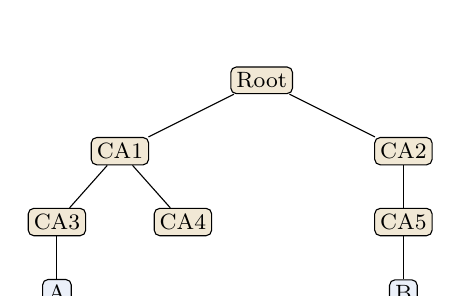
\begin{tikzpicture}[font=\footnotesize, c/.style={draw, rounded corners=2pt, fill=gold!15, inner sep=2pt}, u/.style={draw, rounded corners=2pt, fill=acc!8, inner sep=2pt}]
  \node[c] (r) at (3,0) {Root};
  \node[c] (c1) at (1.2,-0.9) {CA1}; \node[c] (c2) at (4.8,-0.9) {CA2};
  \node[c] (c3) at (0.4,-1.8) {CA3}; \node[c] (c4) at (2.0,-1.8) {CA4}; \node[c] (c5) at (4.8,-1.8) {CA5};
  \node[u] (a) at (0.4,-2.7) {A}; \node[u] (b) at (4.8,-2.7) {B};
  \foreach \x/\y in {r/c1,r/c2,c1/c3,c1/c4,c2/c5,c3/a,c5/b} \draw (\x) -- (\y);
  \end{tikzpicture}
  \end{center}
  (a) User A holds the root's public key. Write the chain A needs to obtain a verified public key of B, and the verification steps. (b) If A trusts only its own issuer CA3, what chain is needed? (c) Write the chain B uses to verify A, trusting only CA5. (d) If five such hierarchies are joined in a mesh by cross-certifying their roots, how many cross-certificates are needed?\\
  \textbf{Solution.} (a) $\text{Root}\langle\!\langle \text{CA2} \rangle\!\rangle\ \text{CA2}\langle\!\langle \text{CA5} \rangle\!\rangle\ \text{CA5}\langle\!\langle B \rangle\!\rangle$. A verifies $\text{Root}\langle\!\langle \text{CA2} \rangle\!\rangle$ with the root's key and extracts CA2's public key; verifies $\text{CA2}\langle\!\langle \text{CA5} \rangle\!\rangle$ with it and extracts CA5's key; verifies $\text{CA5}\langle\!\langle B \rangle\!\rangle$ and extracts B's key. At each step A also checks the validity period and the CRL.\\
  (b) A must first climb to the root through reverse certificates: $\text{CA3}\langle\!\langle \text{CA1} \rangle\!\rangle\ \text{CA1}\langle\!\langle \text{Root} \rangle\!\rangle\ \text{Root}\langle\!\langle \text{CA2} \rangle\!\rangle\ \text{CA2}\langle\!\langle \text{CA5} \rangle\!\rangle\ \text{CA5}\langle\!\langle B \rangle\!\rangle$ (five certificates).\\
  (c) $\text{CA5}\langle\!\langle \text{CA2} \rangle\!\rangle\ \text{CA2}\langle\!\langle \text{Root} \rangle\!\rangle\ \text{Root}\langle\!\langle \text{CA1} \rangle\!\rangle\ \text{CA1}\langle\!\langle \text{CA3} \rangle\!\rangle\ \text{CA3}\langle\!\langle A \rangle\!\rangle$.\\
  (d) Each root certifies each of the other four: $n(n-1) = 5 \cdot 4 = \mathbf{20}$ cross-certificates.\\
  \emph{Check}: each certificate in a chain is verified with the public key extracted from the one before it, and the first with a key the verifier already trusts.

  \item \textbf{(Public-key distribution, 5 marks.)} Explain public announcement, trusted center, controlled trusted center and certification authority as methods of distributing public keys. Which weakness of each does the next one remove?\\
  \textbf{Model answer outline.} Public announcement: Bob publishes his key himself; anyone can forge an announcement in Bob's name. Trusted center: a directory of keys registered securely in person; removes forgery of the registration, but the lookup reply can be intercepted and replaced. Controlled trusted center: replies are signed with the center's private key and contain the request and a timestamp, so they cannot be altered or replayed; but the center must be online for every request (bottleneck, target). Certification authority: the CA signs a certificate (identity, public key, validity) once, in advance; certificates are self-protecting and verified offline with the CA's public key, so the CA need not be online; validity is managed by expiry, renewal and CRLs. (Draw the seven-message public-key authority exchange of \S\ref{sec:pki} for full marks.)
\end{enumerate}

% Question bank for Lecture 17 (entity authentication). All numbers verified by script (scratchpad/w22/verify*.py).
\section{Entity Authentication}\label{q:entityauth}

\subsection*{Check your understanding}
\begin{enumerate}[leftmargin=1.6em,itemsep=3pt]
  \item \textbf{Define entity authentication. Who are the claimant and the verifier?} Entity authentication is a technique that lets one party prove the identity of another party. The entity whose identity must be proved is the claimant; the party that tries to prove the claimant's identity is the verifier. When Bob checks Alice, Alice is the claimant and Bob the verifier.
  \item \textbf{Give the two differences between data-origin (message) authentication and entity authentication.} First, message authentication need not happen in real time (Alice may be offline when Bob checks her e-mail), whereas entity authentication does (Alice must be online and take part before any message flows, as at an ATM). Second, message authentication covers one message and must be repeated for every message, whereas entity authentication covers the claimant for the whole session.
  \item \textbf{Name the three kinds of witness with two examples each. Is ``password plus a security question'' two-factor authentication?} Something known (password, PIN, private key), something possessed (smart card, passport, ATM card), something inherent (fingerprint, retina, voice, signature). Password plus security question is \emph{not} two-factor: both are something known, so one keylogger or one phishing page captures both; two factors must come from two different categories.
  \item \textbf{Why does a system store $h(P)$ instead of $P$? Which attack is still possible, and why do account lock-outs not stop it?} If the file of clear passwords is stolen, every account is lost at once; with hashes, Eve cannot invert $h$ to get $P$, and sending $h(P)$ does not help because the system hashes whatever it receives. The remaining attack is the dictionary attack: Eve hashes every likely password and looks for matches in the stolen file. It runs offline on Eve's own computer, so the system never sees her guesses; lock-outs and delays only limit \emph{online} guessing, and Eve goes online only once, with the password she has already found.
  \item \textbf{What does salting achieve, and what does it not achieve?} The salt, a random string stored in clear beside $h(P \| S)$, makes equal passwords hash differently, multiplies the size of any precomputed table by $2^b$ for a $b$-bit salt (4096 for UNIX's 12 bits), forces the users of one file to be attacked one at a time, and hides password reuse across systems. It does not slow an attack on one chosen user, because that user's salt is in the file; only strong passwords and slow (iterated) hashing help there.
  \item \textbf{What is the weakness of the second one-time-password approach (sequential update)?} Each password $P_{i+1}$ travels encrypted under $P_i$, so the chain can be followed forwards: if Eve guesses or steals $P_1$ (or any $P_i$), she decrypts the recorded traffic and learns all later passwords. The system must also keep the current $P_i$ in usable form, and a lost message desynchronises the two sides.
  \item \textbf{In Lamport's scheme, why can an eavesdropper not use the value she sees?} The values are used in the order $h^{n-1}(P_0), h^{n-2}(P_0), \dots$; after seeing $h^k(P_0)$ Eve needs $h^{k-1}(P_0)$, a preimage of what she holds, which a preimage-resistant hash does not allow. Replaying $h^k(P_0)$ fails because the system now stores it and checks $h(\text{received})$ against it.
  \item \textbf{What is the small-$n$ attack on Lamport's scheme and how is it prevented?} Eve impersonates the server and sends a counter $m$ much smaller than the real one; Alice answers $h^{m-1}(P_0)$, from which Eve can hash forwards to any later chain element the real server will ask for. Alice must refuse a counter that is not smaller than the last one she answered (and should authenticate the server).
  \item \textbf{Differentiate a replay attack and a reflection attack.} A replay attack resends a message recorded in an earlier run and is defeated by freshness (nonce, timestamp, sequence number). A reflection attack sends a party's own message or response back to it in a concurrent run; it is defeated by asymmetry: the claimant answers first, identities or different formats inside responses, or different keys per direction.
  \item \textbf{Compare a nonce and a timestamp as the challenge.} A nonce needs no synchronised clocks or shared state but costs an extra message from the verifier. A timestamp lets the claimant start, so one message suffices, but the clocks must be synchronised and the verifier must remember recent timestamps to stop replays inside the acceptance window.
  \item \textbf{In signature-based challenge--response, why does Alice add her own nonce $R_A$ and Bob's name?} Without $R_A$, Alice would sign any value Bob chooses, which a dishonest verifier could use to obtain her signature on a document of his choosing. The verifier's name prevents Eve from presenting a response signed for Bob to another verifier, Carol.
  \item \textbf{State the three properties of a zero-knowledge proof.} Completeness: an honest claimant who knows the secret is always accepted. Soundness: a claimant without the secret is accepted only with negligible probability, which repetition makes as small as desired. Zero-knowledge: the verifier learns nothing except that the claim is true, because he could have produced every transcript himself.
  \item \textbf{Why must Alice choose a fresh $r$ in every Fiat--Shamir round?} If she uses the same $r$ in two rounds and gets both $c = 0$ and $c = 1$, she reveals $y_0 = r$ and $y_1 = rs$, and then $s = y_1 y_0^{-1} \bmod n$.
  \item \textbf{Differentiate FAR and FRR. What is the equal error rate?} FAR is the fraction of impostor attempts that are wrongly accepted (a security failure); FRR is the fraction of genuine attempts that are wrongly rejected (an inconvenience). Raising the matching threshold lowers FAR and raises FRR; the threshold at which they are equal gives the equal error rate, a single figure for comparing systems.
  \item \textbf{Why can a biometric template not be hashed like a password, and what is the main disadvantage of biometrics?} Two readings of the same feature are never identical, so the system must compute a similarity score against a stored usable template rather than compare hashes for equality. The main disadvantage is that a stolen or copied biometric cannot be changed, unlike a password; privacy of the template database is a further concern.
\end{enumerate}

\subsection*{Practice problems}
\begin{enumerate}[leftmargin=1.6em,itemsep=4pt]
  \item In the Fiat--Shamir protocol, $n = 253$ ($= 11 \times 23$) and Alice's private key is $s = 21$. (a) Find her public key $v$. (b) She chooses $r = 30$. Compute the witness, and the response and Bob's check for $c = 1$ and for $c = 0$. \hfill (4 marks)\\
  \textbf{Solution.} (a) $\gcd(21, 253) = 1$. $v = 21^2 \bmod 253 = 441 - 253 = \mathbf{188}$.\\
  (b) $x = 30^2 \bmod 253 = 900 - 759 = \mathbf{141}$.\\
  $c = 1$: $y = r s = 30 \cdot 21 = 630 \bmod 253 = 630 - 506 = \mathbf{124}$. Bob: $y^2 = 15\,376 = 60 \cdot 253 + 196 \to 196$; $x v = 141 \cdot 188 = 26\,508 = 104 \cdot 253 + 196 \to 196$. Equal, round passed.\\
  $c = 0$: $y = r = \mathbf{30}$. Bob: $y^2 = 900 \bmod 253 = 141 = x = x v^0$. Round passed.\\
  \emph{Check}: $y^2 = r^2 s^{2c} = x v^c$ in both cases.

  \item With $n = 77$ and Alice's public key $v = 4$, Bob receives the witness $x = 15$, sends $c = 1$, and receives $y = 13$. Should he accept the round? What would have happened if he had sent $c = 0$? \hfill (2 marks)\\
  \textbf{Solution.} $y^2 = 169 \bmod 77 = 15$, while $x v^c = 15 \cdot 4 = 60$. Since $15 \ne 60$, Bob \textbf{rejects}. The claimant sent $y = r$ (indeed $13^2 \equiv 15 = x$), which is the correct answer to $c = 0$ only; had Bob sent $c = 0$, the check $y^2 = x$ would have passed. This is exactly a cheater who bet on $c = 0$.\\
  \emph{Check}: the honest answer for $c = 1$ is $y = rs = 13 \cdot 9 \bmod 77 = 40$, with $40^2 \bmod 77 = 60$.

  \item (a) How many Fiat--Shamir rounds make a cheater's success probability less than $10^{-6}$? Less than $10^{-9}$? (b) How many Feige--Fiat--Shamir rounds with $k = 4$ secrets give less than $10^{-6}$? (c) How many Guillou--Quisquater rounds with $e = 3$, and with $e = 65537$? \hfill (4 marks)\\
  \textbf{Solution.} (a) A cheater passes a round with probability $1/2$, so $k$ rounds with $(1/2)^k$. Need $2^k > 10^6$: $\log_2 10^6 = 19.93$, so $\mathbf{20}$ rounds ($2^{-20} = 9.54 \times 10^{-7}$). For $10^{-9}$: $\log_2 10^9 = 29.90$, so $\mathbf{30}$ rounds ($2^{-30} = 9.31 \times 10^{-10}$).\\
  (b) Per round $1/2^4 = 1/16$; need $16^t > 10^6$: $16^4 = 65\,536$, $16^5 = 1\,048\,576$, so $\mathbf{5}$ rounds ($16^{-5} = 9.54 \times 10^{-7}$, the same as 20 Fiat--Shamir rounds).\\
  (c) Per round $1/e$. For $e = 3$: $3^{12} = 531\,441 < 10^6 < 3^{13} = 1\,594\,323$, so $\mathbf{13}$ rounds. For $e = 65537$: $65537^2 = 4\,295\,098\,369 > 10^6$, so $\mathbf{2}$ rounds (probability $2.33 \times 10^{-10}$).\\
  \emph{Check}: rounds needed $= \lceil \log(1/\varepsilon) / \log(\text{choices per round}) \rceil$.

  \item In Feige--Fiat--Shamir, $n = 143$ and Alice's private keys are $[3, 5, 7]$, so her public keys are $[16, 103, 108]$. She chooses $r = 10$ and Bob sends $[0, 1, 1]$. Compute $x$, $y$ and Bob's check. \hfill (3 marks)\\
  \textbf{Solution.} Public keys: $v_i = (s_i^2)^{-1}$: $9 \cdot 16 = 144 \equiv 1$, $25 \cdot 103 = 2575 = 18 \cdot 143 + 1$, $49 \cdot 108 = 5292 = 37 \cdot 143 + 1$ \checkmark.\\
  $x = 10^2 \bmod 143 = \mathbf{100}$. With $c = [0, 1, 1]$: $y = r s_2 s_3 = 10 \cdot 5 \cdot 7 = 350 \bmod 143 = 350 - 286 = \mathbf{64}$.\\
  Bob computes $y^2 v_2 v_3$: $64^2 = 4096 = 28 \cdot 143 + 92 \to 92$; $92 \cdot 103 = 9476 = 66 \cdot 143 + 38 \to 38$; $38 \cdot 108 = 4104 = 28 \cdot 143 + 100 \to \mathbf{100} = x$. Accepted.\\
  \emph{Check}: $y^2 \prod v_i^{c_i} = x \prod (s_i^2 v_i)^{c_i} = x$.

  \item In Guillou--Quisquater, $n = 77$ ($= 7 \times 11$), $e = 7$, and Alice's secret is $s = 2$. (a) Verify that $e$ is valid and find Alice's public key $v$. (b) She picks $r = 3$ and Bob sends $c = 2$. Compute $x$, $y$ and Bob's check. \hfill (5 marks)\\
  \textbf{Solution.} (a) $\phi = 6 \times 10 = 60$; $\gcd(7, 60) = 1$, so $e = 7$ is valid. $s^e = 2^7 = 128 \bmod 77 = 51$. $v = 51^{-1} \bmod 77$ by extended Euclid on $(77, 51)$: quotients $1, 1, 1, 25$; remainders $26, 25, 1, 0$; $t$-values $-1, 2, -3$. So $v = -3 + 77 = \mathbf{74}$. Check: $51 \cdot 74 = 3774 = 49 \cdot 77 + 1$ \checkmark.\\
  (b) $x = 3^7 \bmod 77 = 2187 - 28 \cdot 77 = 2187 - 2156 = \mathbf{31}$. $y = r s^c = 3 \cdot 2^2 = \mathbf{12}$.\\
  Bob: $y^7$: $12^2 = 144 \to 67$; $12^4 = 67^2 = 4489 \to 23$; $12^7 = 12^4 \cdot 12^2 \cdot 12$: $23 \cdot 67 = 1541 \to 1$, $1 \cdot 12 = 12$. $v^2 = 74^2 = 5476 = 71 \cdot 77 + 9 \to 9$. $y^e v^c = 12 \cdot 9 = 108 \bmod 77 = \mathbf{31} = x$. Accepted.\\
  \emph{Check}: $y^e v^c = r^e (s^e v)^c = x \cdot 1^c$.

  \item Lamport's scheme uses the toy hash $h(x) = x^2 \bmod 1003$. Alice's original password is $P_0 = 25$ and $n = 4$. (a) Compute the hash chain and the entry stored by the system. (b) Show the first two logins and the stored entry after each. (c) Eve records the value sent in the first login. What can she compute from it, and why can she not log in? (d) How many logins are possible? \hfill (5 marks)\\
  \textbf{Solution.} (a) $h^1 = 25^2 = 625$; $h^2 = 625^2 = 390\,625 = 389 \cdot 1003 + 458 \to 458$; $h^3 = 458^2 = 209\,764 = 209 \cdot 1003 + 137 \to 137$; $h^4 = 137^2 = 18\,769 = 18 \cdot 1003 + 715 \to 715$. Stored entry: \textbf{(Alice, 4, 715)}.\\
  (b) Login 1: system sends 4; Alice sends $h^3(P_0) = 137$; system checks $137^2 \bmod 1003 = 715$ \checkmark; new entry \textbf{(Alice, 3, 137)}. Login 2: system sends 3; Alice sends $h^2(P_0) = 458$; $458^2 \bmod 1003 = 137$ \checkmark; new entry \textbf{(Alice, 2, 458)}.\\
  (c) From 137 Eve can only hash forwards: $h(137) = 715$, $h(715) = 698$, values that are already used or never asked. At login 2 she needs $h^2(P_0) = 458$, a square root of 137 modulo 1003, i.e.\ a preimage; replaying 137 gives $137^2 \bmod 1003 = 715 \ne 137$ and is rejected.\\
  (d) $n = 4$ logins (the last one sends $P_0 = 25$ itself); then the counter is 0 and the system must be re-initialised.

  \item A UNIX-style system uses a 12-bit salt. Eve's dictionary has $2^{20}$ words and she computes $2^{20}$ hashes per second. (a) How many entries does a precomputed table for all salts need, and how long does building it take? (b) The stolen file has $2^{10}$ users with distinct salts. How long does it take to test the dictionary against all of them, with and without salt? (c) How long for one targeted user? \hfill (4 marks)\\
  \textbf{Solution.} (a) $2^{20} \times 2^{12} = 2^{32} = \mathbf{4\,294\,967\,296}$ entries, $2^{12} = 4096$ times the unsalted table; building it takes $2^{32}/2^{20} = 2^{12} = 4096$ s $\approx \mathbf{1.14}$ \textbf{hours}.\\
  (b) Without salt: one pass of $2^{20}$ hashes, each looked up among the stored hashes: $\mathbf{1}$ \textbf{s}. With distinct salts: one pass per user, $2^{10} \times 2^{20} = 2^{30}$ hashes $= 1024$ s $\approx \mathbf{17}$ \textbf{minutes}.\\
  (c) Her salt is in the file, so one pass of $2^{20}$ hashes: $\mathbf{1}$ \textbf{s}, the same as without salt.\\
  \emph{Check}: salting multiplies the bulk attack by the number of distinct salts and precomputation by $2^{12}$, but not the single-user attack.

  \item Passwords are 8 characters drawn from the 62 letters and digits, and the stored hashes are unsalted. Eve can compute $10^9$ hashes per second. (a) How long does an exhaustive offline search take? (b) How much longer for 9 characters? (c) An ATM card is blocked after 3 wrong 4-digit PINs; what is a thief's chance of success? \hfill (3 marks)\\
  \textbf{Solution.} (a) $62^8 = 218\,340\,105\,584\,896 \approx 2.18 \times 10^{14}$ hashes; $2.18 \times 10^{14} / 10^9 = 2.18 \times 10^5$ s $\approx 60.7$ hours $\approx \mathbf{2.5}$ \textbf{days}.\\
  (b) One more character multiplies the work by 62: $\approx \mathbf{157}$ \textbf{days}.\\
  (c) Three distinct guesses out of $10^4$ PINs: $3/10^4 = \mathbf{0.03\%}$. The short PIN is safe only because guessing is online and limited; offline, $10^4$ hashes would take microseconds.

  \item A face-recognition system is tested with 2000 genuine attempts, of which 50 are rejected, and 8000 impostor attempts, of which 4 are accepted. (a) Compute FRR and FAR. (b) The system is used for identification against 1000 enrolled faces with this FAR per comparison. What is the probability that an impostor matches someone? (c) What happens to both rates if the threshold is raised? \hfill (3 marks)\\
  \textbf{Solution.} (a) $\mathrm{FRR} = 50/2000 = \mathbf{2.5\%}$; $\mathrm{FAR} = 4/8000 = \mathbf{0.05\%}$.\\
  (b) $1 - (1 - 0.0005)^{1000} = 1 - 0.6065 = \mathbf{0.394}$ (about $1 - e^{-0.5}$, since $1000 \times 0.0005 = 0.5$ false matches are expected).\\
  (c) A stricter threshold lowers FAR and raises FRR; the rates are equal at the equal error rate.

  \item Draw and explain challenge--response mutual authentication using a symmetric-key cipher. Show a reflection attack on the version in which the initiator challenges first, and state how to prevent it. \hfill (6 marks)\\
  \textbf{Solution (model answer outline).} Draw the four-message diagram of \S\ref{sec:entityauth}: (1) Alice; (2) $R_B$; (3) $E_{K_{AB}}(R_A \| R_B)$; (4) $E_{K_{AB}}(R_B \| R_A)$. Explain: message 3 proves Alice knows $K_{AB}$ (contains Bob's fresh nonce) and carries her challenge; message 4 proves Bob knows $K_{AB}$; fresh nonces stop replay. Then the vulnerable protocol: (1) Alice, $R_A$; (2) $E_K(R_A)$, $R_B$; (3) $E_K(R_B)$. Attack in two sessions: S1: Eve sends ``Alice'', $R_E$, gets $E_K(R_E)$, $R_B$; S2: Eve sends ``Alice'', $R_B$, gets $E_K(R_B)$; she returns $E_K(R_B)$ in S1 and is accepted. Prevention: claimant proves first; identities or different formats inside the ciphertext ($E_K(R_B, \text{Bob})$); different keys per direction.

  \item Explain the Fiat--Shamir zero-knowledge protocol with a diagram. Prove that an honest claimant always passes, and show that a dishonest claimant passes a round with probability $1/2$. \hfill (6 marks)\\
  \textbf{Solution (model answer outline).} Setup: trusted party publishes $n = pq$; Alice's secret $s$ (coprime to $n$), public $v = s^2 \bmod n$. Diagram: $x = r^2$ (witness) $\to$; $\leftarrow c \in \{0, 1\}$; $y = r s^c \to$; Bob checks $y^2 \equiv x v^c$. Proof: $y^2 = r^2 s^{2c} = x v^c$. Cheater: guessing $c = 1$, send $x = r^2 v^{-1}$ and $y = r$; guessing $c = 0$, send $x = r^2$ and $y = r$; each passes only if the guess is right. She cannot answer both for one $x$, since $y_0^2 = x$, $y_1^2 = xv$ give $(y_1/y_0)^2 = v$, a square root of $v$ (as hard as factoring $n$). Hence probability $1/2$ per round, $(1/2)^k$ after $k$ rounds (20 rounds: $9.54 \times 10^{-7}$). Mention the zero-knowledge property and the need for a fresh $r$.

  \item Explain biometric authentication: enrollment, verification and identification, the two classes of techniques with examples, and the two accuracy measures. \hfill (5 marks)\\
  \textbf{Solution (model answer outline).} Definition: measurement of physiological or behavioural features (something inherent). Components: capturing device, processor (feature extraction, template, matching), storage. Enrollment: each person's template recorded in the database before use. Verification: 1:1 match against the claimed identity's record (bank checks a signature on a cheque); identification: 1:N match against all records (employee-only building). Draw the enrollment/authentication flow with the threshold decision. Physiological: fingerprint, iris, retina, face, hands, voice, DNA; behavioural: signature, keystroke. Accuracy: FRR $=$ false rejections / genuine attempts; FAR $=$ false acceptances / impostor attempts; threshold trade-off and EER. Close with advantages (cannot be forgotten or lent) and disadvantages (cannot be changed if stolen, copying, privacy).
\end{enumerate}

% Question bank for Lecture 18 (DNA, quantum cryptography, steganography, watermarking).
% Every number recomputed by script (scratchpad/w23/verify.py, quantum.py, qverify.py).
\section{Other Cryptographic Techniques}\label{q:othertech}
\noindent{\small Notes: \S\ref{sec:othertech}.}

\subsection*{Check your understanding}
\begin{enumerate}[leftmargin=1.6em,itemsep=3pt]
  \item \textbf{Why is DNA attractive for cryptography?} One chemical step acts on trillions of strands at once (massive parallelism), DNA stores about 1 bit per nm$^3$, roughly $10^{12}$ times denser than conventional media (about 456 exabytes per gram at 2 bits per nucleotide), hybridisation needs almost no energy, and security can rest on a biological difficulty such as not knowing the primer needed to find and amplify a hidden strand.
  \item \textbf{State the base-pairing rule and its binary meaning.} A pairs with T (two hydrogen bonds) and C pairs with G (three), and the two strands are antiparallel ($5'\to3'$ against $3'\to5'$). With A $= 00$, C $= 01$, G $= 10$, T $= 11$, the Watson--Crick complement of a strand is exactly the bitwise NOT of its binary code, since $00 \leftrightarrow 11$ and $01 \leftrightarrow 10$.
  \item \textbf{Why are only 8 of the $4! = 24$ binary encodings of A, C, G, T complementary?} Complementary bases must receive complementary 2-bit values, so \{A, T\} gets one of the pairs \{00, 11\} or \{01, 10\} and \{C, G\} the other (2 ways), each pair can be ordered in 2 ways inside \{A, T\} and 2 ways inside \{C, G\}: $2 \times 2 \times 2 = 8$.
  \item \textbf{What does the slide's complementary rule do, and does it add security?} A$\to$C$\to$G$\to$T$\to$A adds 1 modulo 4 to each 2-bit group; it is a fixed public bijection with no key, so by Kerckhoffs's principle Eve undoes it herself. All the security of the algorithm comes from the XOR with the key: perfect with a true one-time pad, trivial with a one-byte key from 1 to 256.
  \item \textbf{What did Adleman's 1994 experiment show, and why is it not a practical computer?} He solved a 7-vertex Hamiltonian path problem by encoding vertices and edges as DNA strands, letting hybridisation and ligation build all paths at once, and filtering with PCR (correct ends), gel electrophoresis (length 140 bases) and affinity separation (every vertex present). The search was parallel, but the laboratory steps took about a week and the amount of DNA grows exponentially with the graph size.
  \item \textbf{What are the main limitations of DNA cryptography?} Expensive laboratory equipment, slow operations (hours to days), error-prone synthesis, hybridisation and sequencing, no formal security model, and digital ``pseudo-DNA'' schemes are only as strong as the classical cipher inside them.
  \item \textbf{What is a qubit, and what happens when it is measured?} A qubit is a two-level quantum system, in QKD a single photon, whose state $\alpha\lvert 0\rangle + \beta\lvert 1\rangle$ with $|\alpha|^2 + |\beta|^2 = 1$ can be a superposition. Measuring it gives 0 with probability $|\alpha|^2$ and 1 with probability $|\beta|^2$ and leaves it in the observed state, so measurement disturbs it; a photon measured in a basis at $45^\circ$ to its polarisation gives a random result.
  \item \textbf{State the no-cloning theorem and its role in QKD.} An unknown quantum state cannot be copied: a copier $U$ for two states $\lvert\psi\rangle, \lvert\varphi\rangle$ would force $\langle\varphi|\psi\rangle = \langle\varphi|\psi\rangle^2$, so it works only for identical or orthogonal states. Eve therefore cannot copy a photon and measure the copy later; she must measure the original and, if she uses the wrong basis, disturb it. It also forbids amplifying photons on long links.
  \item \textbf{Why does an intercept--resend eavesdropper cause 25\% errors in the BB84 sifted key?} For a sifted bit Eve uses the wrong basis with probability $1/2$; she then resends a photon at $45^\circ$ to Alice's basis, and Bob, measuring in Alice's basis, is wrong with probability $1/2$. Error rate $= \frac12 \times \frac12 = \frac14$ (and $f/4$ if she attacks a fraction $f$ of the photons).
  \item \textbf{Why must BB84's public channel be authenticated, though not secret?} The public messages reveal only bases, positions and test bits, which do not give away the key, so secrecy is unnecessary. But if Eve could alter them she would run BB84 separately with Alice and with Bob (man in the middle) and no error would appear; hence a pre-shared key or signature is needed, which makes QKD a key-expansion method.
  \item \textbf{Differentiate the impact of Shor's and Grover's algorithms.} Shor's algorithm factors and computes discrete logarithms (also on elliptic curves) in polynomial time, so RSA, Diffie--Hellman, ElGamal, DSA and ECC are broken outright. Grover's algorithm searches $N$ items in about $\frac{\pi}{4}\sqrt N$ steps, so a $k$-bit key gives only $k/2$ bits of security; symmetric ciphers survive by doubling the key length (AES-256).
  \item \textbf{What is post-quantum cryptography and how does it differ from quantum cryptography?} PQC is classical software whose security rests on problems believed hard even for quantum computers: lattices (ML-KEM/Kyber, FIPS 203; ML-DSA/Dilithium, FIPS 204), hash-based signatures (SLH-DSA/SPHINCS$^+$, FIPS 205) and codes (McEliece, HQC). Quantum cryptography (QKD) uses physics, needs special hardware and dedicated links, and provides only key exchange.
  \item \textbf{Why is QKD hard over long distances?} Fibre loses about 0.2 dB per km, so only $10^{-0.02L}$ of the photons survive $L$ km (1\% at 100 km, $10^{-10}$ at 500 km), and the signal cannot be amplified because amplification would clone unknown quantum states; long links need trusted relay nodes or satellites.
  \item \textbf{Differentiate cryptography, steganography and watermarking.} Cryptography hides the meaning of a message (ciphertext is visibly secret; attacked by cryptanalysis). Steganography hides the existence of a message inside a cover for secret communication; it needs undetectability and capacity and is defeated by detection (steganalysis). Watermarking embeds information about the cover itself (owner, buyer) for copyright and authentication; it may be visible and needs robustness, and is defeated only by removal or forgery.
  \item \textbf{Differentiate robust, fragile and semi-fragile watermarks.} A robust watermark survives compression, filtering and attacks and serves copyright and fingerprinting; a fragile watermark breaks at any modification and so proves tampering; a semi-fragile one survives benign processing such as JPEG compression but breaks under content changes, which suits photo authentication.
  \item \textbf{Why is LSB steganography imperceptible but fragile and detectable?} Each value changes by at most 1 in 255 (PSNR $\ge 48.1$ dB, about 51 dB for random bits), so nothing is visible; but compression or resizing rewrites the low bits, and since LSB replacement only moves values within pairs $\{2i, 2i+1\}$, the histogram counts of each pair become equal, which the chi-square attack detects.
\end{enumerate}

\subsection*{Practice problems}
\begin{enumerate}[leftmargin=1.6em,itemsep=4pt]
  \item Using the DNA cryptography algorithm of the lecture (A $= 00$, C $= 01$, G $= 10$, T $= 11$; complementary rule A$\to$C, C$\to$G, G$\to$T, T$\to$A; XOR with a one-time-pad key; result written as DNA bases), encrypt the plaintext ``GO'' with the key ``AB'' and decrypt the result. \hfill (5 marks)\\
  \textbf{Solution.} Steps 1--4 (ASCII, binary, DNA, rule, binary):\\
  \ttx{G} $= 71 = $ \ttx{01000111} $\to$ \ttx{CACT} $\to$ \ttx{GCGA} $\to$ \ttx{10011000};\quad \ttx{O} $= 79 = $ \ttx{01001111} $\to$ \ttx{CATT} $\to$ \ttx{GCAA} $\to$ \ttx{10010000}.\\
  Key: \ttx{A} $= 65 = $ \ttx{01000001}, \ttx{B} $= 66 = $ \ttx{01000010}.\\
  XOR: \ttx{10011000} $\oplus$ \ttx{01000001} $= $ \ttx{11011001} $\to$ \ttx{TCGC};\quad \ttx{10010000} $\oplus$ \ttx{01000010} $= $ \ttx{11010010} $\to$ \ttx{TCAG}.\\
  Ciphertext: \textbf{\ttx{TCGCTCAG}}.\\
  Decryption: \ttx{TCGC} $\to$ \ttx{11011001} $\oplus$ \ttx{01000001} $= $ \ttx{10011000} $\to$ \ttx{GCGA} $\to$ (inverse rule) \ttx{CACT} $\to$ \ttx{01000111} $= 71 = $ \ttx{G}; \ttx{TCAG} $\to$ \ttx{11010010} $\oplus$ \ttx{01000010} $= $ \ttx{10010000} $\to$ \ttx{GCAA} $\to$ \ttx{CATT} $\to$ \ttx{01001111} $= 79 = $ \ttx{O}. Recovered \textbf{GO}.\\
  \emph{Check}: XOR is its own inverse and the inverse rule (C$\to$A, G$\to$C, T$\to$G, A$\to$T) undoes the forward rule base by base.

  \item With the same algorithm, decrypt the DNA ciphertext \ttx{TCGATAGC} using the one-time-pad key ``KY''. \hfill (4 marks)\\
  \textbf{Solution.} Key bytes: \ttx{K} $= 75 = $ \ttx{01001011}, \ttx{Y} $= 89 = $ \ttx{01011001}.\\
  \ttx{TCGA} $\to$ \ttx{11011000}; $\oplus$ \ttx{01001011} $= $ \ttx{10010011} $\to$ \ttx{GCAT} $\to$ inverse rule \ttx{CATG} $\to$ \ttx{01001110} $= 78 = $ \ttx{N}.\\
  \ttx{TAGC} $\to$ \ttx{11001001}; $\oplus$ \ttx{01011001} $= $ \ttx{10010000} $\to$ \ttx{GCAA} $\to$ \ttx{CATT} $\to$ \ttx{01001111} $= 79 = $ \ttx{O}.\\
  Plaintext: \textbf{NO}. \emph{Check}: re-encrypting \ttx{N}: \ttx{CATG} $\to$ \ttx{GCAT} $=$ \ttx{10010011}, $\oplus$ \ttx{01001011} $=$ \ttx{11011000} $=$ \ttx{TCGA} \checkmark.

  \item (a) Encode the word ``Hi'' as a DNA strand using A $= 00$, C $= 01$, G $= 10$, T $= 11$. (b) Write its Watson--Crick complement and its reverse complement, and show that the complement equals the bitwise NOT of the binary code. (c) How many 4-base words exist, and why are 4 bases enough for one ASCII character? \hfill (4 marks)\\
  \textbf{Solution.} (a) \ttx{H} $= 72 = $ \ttx{01 00 10 00} $=$ \ttx{CAGA}; \ttx{i} $= 105 = $ \ttx{01 10 10 01} $=$ \ttx{CGGC}. Strand: \textbf{\ttx{5'-CAGACGGC-3'}}.\\
  (b) Complement (A$\leftrightarrow$T, C$\leftrightarrow$G): \ttx{3'-GTCTGCCG-5'}; reverse complement (read $5'\to3'$): \textbf{\ttx{5'-GCCGTCTG-3'}}. The binary code is \ttx{0100100001101001}; its NOT is \ttx{1011011110010110} $=$ \ttx{GTCTGCCG}, the complement.\\
  (c) $4^4 = 256 = 2^8$ words, exactly one per 8-bit value, since each base carries 2 bits.

  \item In BB84, Alice sends 12 photons with bits \ttx{100111001011} and bases $\times\,+\,+\,\times\,\times\,+\,\times\,\times\,+\,+\,\times\,+$. Bob measures with bases $+\,+\,+\,\times\,+\,\times\,\times\,\times\,+\,\times\,+\,+$. (a) Give the polarisation of each photon. (b) Which positions are kept after sifting, and what is the sifted key? (c) How many bits would you expect to keep on average? \hfill (5 marks)\\
  \textbf{Solution.} (a) Bit 0/1 is $0^\circ$/$90^\circ$ in $+$ and $45^\circ$/$135^\circ$ in $\times$: $135^\circ, 0^\circ, 0^\circ, 135^\circ, 135^\circ, 90^\circ, 45^\circ, 45^\circ, 90^\circ, 0^\circ, 135^\circ, 90^\circ$.\\
  (b) Bases agree at positions \textbf{2, 3, 4, 7, 8, 9, 12} (at 1, 5, 6, 10, 11 they differ and Bob's results are random). Bob's results there equal Alice's bits: sifted key \textbf{\ttx{0010011}} (7 bits).\\
  (c) Each basis pair agrees with probability $1/2$, so $12/2 = 6$ on average; 7 is a normal fluctuation.\\
  \emph{Check}: Bob announces only his bases and Alice only the matching positions, so no bit value is revealed during sifting.

  \item Eve performs an intercept--resend attack on 40\% of the photons in a BB84 session. (a) What QBER does this cause? (b) Alice and Bob compare 50 sifted bits; how many errors do they expect, and what is the probability that they see none? (c) Compare with Eve attacking every photon. \hfill (4 marks)\\
  \textbf{Solution.} (a) A sifted bit has an error only if Eve attacked it (probability $f$), chose the wrong basis ($\frac12$) and Bob's result flipped ($\frac12$): QBER $= f/4 = 0.4/4 = \mathbf{0.10} = 10\%$.\\
  (b) Expected errors $= 50 \times 0.1 = \mathbf{5}$; $\Pr[\text{no error}] = 0.9^{50} = \mathbf{0.00515}$.\\
  (c) With $f = 1$: QBER $= 25\%$, $\Pr[\text{no error in 50}] = 0.75^{50} = 5.66 \times 10^{-7}$.\\
  \emph{Check}: a 10\% QBER is below the roughly 11\% abort threshold, so the key may still be usable, but privacy amplification must shorten it a lot to remove Eve's information.

  \item A $512 \times 512$ 24-bit colour image is used as a cover for LSB steganography. (a) What is the capacity in bytes with one LSB per colour component, and with two? (b) How many pixels are needed to hide a 2 KB file at one LSB per component? (c) Why is the change invisible? \hfill (4 marks)\\
  \textbf{Solution.} (a) $512 \times 512 = 262\,144$ pixels $\times$ 3 bits $= 786\,432$ bits $= \mathbf{98\,304}$ \textbf{bytes} (96 KiB); with 2 LSBs, $\mathbf{196\,608}$ bytes.\\
  (b) $2048 \times 8 = 16\,384$ bits $/ 3 = 5461.3$, so \textbf{5462 pixels}.\\
  (c) Each component changes by at most 1, so $\mathrm{MSE} \le 1$ and $\mathrm{PSNR} = 10\log_{10}(255^2/\mathrm{MSE}) \ge 48.1$ dB (about 51.1 dB for random message bits, since only half the LSBs change).

  \item Decrypt the Caesar ciphertext ``esp aszezy nlyyze mp nwzypo'', given that the plaintext begins with ``the''. \hfill (3 marks)\\
  \textbf{Solution.} $k = \mathrm{e} - \mathrm{t} = 4 - 19 = -15 \equiv 11 \pmod{26}$ (check: $\mathrm{s} - \mathrm{h} = 18 - 7 = 11$, $\mathrm{p} - \mathrm{e} = 15 - 4 = 11$). Shifting every letter back by 11: \textbf{``the photon cannot be cloned''}.\\
  \emph{Check}: re-encrypting ``be'' with $+11$ gives ``mp''.

  \item Show how Shor's algorithm factors $N = 35$ using $a = 2$, assuming the quantum computer returns the order of $a$. \hfill (4 marks)\\
  \textbf{Solution.} Powers of 2 modulo 35: $2, 4, 8, 16, 32, 29, 23, 11, 22, 9, 18, 1$, so the order is $r = 12$ (even). $a^{r/2} = 2^6 = 64 \equiv 29 \not\equiv -1 \pmod{35}$. Since $(2^6 - 1)(2^6 + 1) \equiv 0 \pmod{35}$, $\gcd(29 - 1, 35) = \gcd(28, 35) = \mathbf{7}$ and $\gcd(29 + 1, 35) = \gcd(30, 35) = \mathbf{5}$.\\
  \emph{Check}: $5 \times 7 = 35$.

  \item A quantum computer performs $10^9$ Grover iterations per second. Estimate the time to recover (a) a 56-bit DES key and (b) a 128-bit AES key with Grover's algorithm. What key length restores 128-bit security? \hfill (3 marks)\\
  \textbf{Solution.} Grover needs about $\frac{\pi}{4}\sqrt{2^k}$ iterations.\\
  (a) $\frac{\pi}{4} 2^{28} = 2.11 \times 10^8$ iterations $\Rightarrow$ \textbf{0.21 s}.\\
  (b) $\frac{\pi}{4} 2^{64} = 1.45 \times 10^{19}$ iterations $\Rightarrow 1.45 \times 10^{10}$ s $\approx$ \textbf{459 years} (still infeasible, but only a 64-bit margin).\\
  A 256-bit key (AES-256) gives $2^{128}$ Grover iterations, i.e.\ 128-bit security.

  \item (a) A PCR reaction starts with 100 template strands. How many copies exist after 25 cycles? (b) Using 2 bits per nucleotide and 330 g/mol per nucleotide, how many grams of DNA would store one zettabyte ($10^{21}$ bytes)? \hfill (3 marks)\\
  \textbf{Solution.} (a) Each cycle doubles the number: $100 \times 2^{25} = \mathbf{3.36 \times 10^9}$ copies.\\
  (b) One gram holds $(6.022 \times 10^{23}/330) \times 2 = 3.65 \times 10^{21}$ bits $= 4.56 \times 10^{20}$ bytes, so $10^{21}/4.56 \times 10^{20} \approx \mathbf{2.2}$ \textbf{grams}.

  \item Explain the BB84 quantum key distribution protocol with a diagram. How does it detect an eavesdropper? \hfill (6 marks)\\
  \textbf{Model answer outline.} (1) Two channels: quantum (photons) and public authenticated classical. (2) Table of the two bases: $+$ ($0^\circ = 0$, $90^\circ = 1$), $\times$ ($45^\circ = 0$, $135^\circ = 1$). (3) Steps: Alice's random bits and bases; Bob's random bases; sifting (Bob announces bases, Alice confirms matches, about half kept); error estimation on a sample (QBER); error correction; privacy amplification. (4) Message-sequence diagram Alice $\to$ Bob (photons), Bob $\to$ Alice (bases), Alice $\to$ Bob (matching positions), sample comparison. (5) A 6--10 photon example table. (6) Detection: measurement disturbs and photons cannot be cloned; intercept--resend gives QBER $= \frac12 \cdot \frac12 = 25\%$, detected in $m$ test bits with probability $1 - (3/4)^m$. (Notes \S\ref{sec:othertech}, BB84 subsections.)

  \item What is digital watermarking? Explain the embedding and detection process, the types of watermark, and four applications. Differentiate it from steganography. \hfill (6 marks)\\
  \textbf{Model answer outline.} (1) Definition: information about the media embedded so that the media looks unchanged; protects the cover, not the message. (2) Block diagram: cover $+$ watermark $+$ key $\to$ embedding $\to$ marked media $\to$ channel/attacks $\to$ detection with key (and original if non-blind) $\to$ watermark present / ID. (3) Properties: imperceptibility, robustness, capacity, security, low false positives, and their trade-off. (4) Types: visible/invisible; robust/fragile/semi-fragile; blind/non-blind; spatial/frequency domain. (5) Applications: owner identification, copy protection (copy-protect bit), photographers' proofs, broadcast monitoring, data authentication, fingerprinting. (6) Table versus steganography: goal, what is valuable, relation to the cover, visibility, requirement (robustness vs undetectability), payload, what counts as a successful attack.
\end{enumerate}

% Question bank for sections/16b_modes.tex and sections/24_network_security.tex (syllabus topics not on the slides).
% Every number checked by scratchpad/w24/modes.py, qcalc.py, net.py.
\section{Modes of Operation, Network and System Security}\label{q:netsec}
\noindent{\small Notes: \S\ref{sec:modes} (modes), \S\ref{sec:netsec}--\S\ref{sec:syssec} (e-mail, IPSec, TLS, SET, system security).}

\subsection*{Check your understanding}
\begin{enumerate}[leftmargin=1.6em,itemsep=3pt]
  \item \textbf{Why is ECB insecure for long messages, and how does CBC fix it?} In ECB equal plaintext blocks always give equal ciphertext blocks, so repetitions and structure of the message show through and blocks can be swapped or replayed. CBC XORs each plaintext block with the previous ciphertext block (the IV for the first) before encrypting, so equal blocks encrypt differently and every ciphertext block depends on all earlier plaintext.
  \item \textbf{Why do CFB, OFB and CTR use only the encryption function at both ends?} In these modes the block cipher only produces a key stream that is XORed with the data; the receiver must regenerate the same key stream, which needs the same $E_K$ on the same inputs, and XORing it again cancels it. $D_K$ is never needed, so the block function need not even be invertible.
  \item \textbf{Differentiate CFB and OFB.} CFB feeds the \emph{ciphertext} back into the shift register, so it is a self-synchronising stream cipher: a bit error damages $1 + n/s$ segments and a lost segment is recovered from after $n/s$ segments. OFB feeds the cipher \emph{output} back, so the key stream is independent of the message: a bit error damages only that bit, but a lost bit desynchronises everything after it, and the key stream can be precomputed.
  \item \textbf{One bit of $C_i$ is flipped in CBC. Which plaintext blocks are wrong, and why?} $P_i = D_K(C'_i) \oplus C_{i-1}$ is completely garbled because the block decryption of a changed block is unrelated to the original; $P_{i+1} = D_K(C_{i+1}) \oplus C'_i$ has exactly the same bit flipped; $P_{i+2}$ onwards are correct because they do not use $C_i$.
  \item \textbf{What happens if the same IV is used twice in OFB (or the same counter in CTR)?} Both messages are XORed with the same key stream, so $C \oplus C' = P \oplus P'$: Eve obtains the XOR of the plaintexts without the key, and knowing one plaintext reveals the other completely.
  \item \textbf{Why must the CBC IV be unpredictable and protected?} A reused IV shows when two messages start with the same block, and a predictable IV lets a chosen-plaintext attacker test a guess $G$ of an old $P_1$ by submitting $\mathrm{IV}' \oplus \mathrm{IV} \oplus G$. Since $P_1 = D_K(C_1) \oplus \mathrm{IV}$, an attacker who changes the IV in transit flips chosen bits of $P_1$.
  \item \textbf{Why does double DES give only about 57-bit security, and why is 3DES EDE?} The meet-in-the-middle attack tabulates $E_{K_1}(P)$ for all $2^{56}$ keys and matches $D_{K_2}(C)$ for all $2^{56}$ keys, costing $2^{57}$ operations (and $2^{56}$ memory) instead of $2^{112}$. EDE with $K_1 = K_2$ reduces to single DES, so 3DES equipment stays compatible with DES.
  \item \textbf{Why does PGP sign before compressing and compress before encrypting?} Signing the uncompressed message lets the signature be stored and verified with the plain message and makes it independent of the (non-deterministic) compression algorithm; compressing before encrypting removes redundancy that cryptanalysis could exploit and shortens the data to encrypt (ciphertext would not compress anyway).
  \item \textbf{What is a PGP key ID and why is it used?} The least significant 64 bits of a public key; it tells the recipient which of several key pairs was used for the session key or the signature without sending the whole public key.
  \item \textbf{Differentiate owner trust and key legitimacy in PGP.} Owner trust, assigned by the user, says how far the key's owner is trusted to sign other people's keys; key legitimacy, computed by PGP from the trust of the signatures on the key, says how far the key is believed to belong to its user ID.
  \item \textbf{Differentiate AH and ESP.} AH provides integrity, origin authentication and anti-replay, and its MAC also covers the immutable fields of the IP header, but it gives no confidentiality; ESP provides encryption (confidentiality), optional authentication and anti-replay, and its authentication covers only the ESP header, payload and trailer, not the IP header in front.
  \item \textbf{Differentiate transport mode and tunnel mode.} Transport mode protects only the IP payload, keeps the original IP header and is used end to end between hosts; tunnel mode protects the entire original packet inside a new IP packet, hides the inner addresses and is used between security gateways (VPN).
  \item \textbf{What is a security association and how is it identified?} A one-way relationship between sender and receiver that defines the security services (AH or ESP, algorithms, keys, lifetime) for its traffic; it is identified by the SPI, the IP destination address and the security protocol identifier (AH or ESP).
  \item \textbf{How do Oakley cookies stop a clogging attack?} The responder sends a cookie (a keyed hash of the addresses, ports and a local secret) to the claimed source address and performs the Diffie--Hellman exponentiation only after the cookie is echoed; an attacker using forged addresses never receives the cookie, so he can only make the victim compute cheap hashes.
  \item \textbf{What does the TLS Finished message achieve?} It is the first message protected under the new keys and contains a PRF value of the master secret and the whole handshake transcript; checking it confirms that both sides have the same keys and that no handshake message (e.g.\ the cipher-suite list) was altered.
  \item \textbf{Differentiate an SSL session and an SSL connection.} A session is an association created by the handshake that fixes the security parameters and master secret and can be shared by many connections; a connection is a transient peer-to-peer transport with its own keys, MAC secrets, IVs and sequence numbers, always belonging to one session.
  \item \textbf{What is a dual signature and why does SET need it?} $\mathrm{DS} = E(PR_c, H(H(\mathrm{PI}) \| H(\mathrm{OI})))$; it links the payment information and the order information so that the customer can prove the payment is for this order, while the merchant sees only OI and $H(\mathrm{PI})$ and the bank only PI and $H(\mathrm{OI})$.
  \item \textbf{Name the four phases of a virus.} Dormant (idle until an event), propagation (copies itself into other programs or system areas), triggering (activated by an event or count), execution (performs its function, harmless or damaging).
  \item \textbf{Differentiate a virus and a worm.} A virus is a fragment that needs a host program and spreads when infected programs are run or shared; a worm is an independent program that propagates itself over the network (e-mail, remote execution, remote login) without a host.
  \item \textbf{Differentiate a packet filter and an application-level gateway.} A packet filter decides per packet from IP/TCP header fields, so it is fast and transparent but blind to application content; an application-level gateway relays traffic through a proxy for each allowed application, so it can authenticate users, restrict commands and log everything, at the cost of processing overhead.
  \item \textbf{State the Bell--LaPadula rules and why both are needed.} No read up (a subject reads only objects at its level or below) and no write down (a subject writes only to objects at its level or above). No read up alone would let a high subject copy what it reads into a low object; the $*$-property blocks that, so information can only flow upwards.
  \item \textbf{What are the three properties of a reference monitor?} Complete mediation (every access is checked), isolation (the monitor and its database cannot be modified by attackers) and verifiability (its correctness can be proved).
\end{enumerate}

\subsection*{Practice problems}
\begin{enumerate}[leftmargin=1.6em,itemsep=4pt]
  \item Use the toy cipher of \S\ref{sec:modes} with $K = 0001$, whose table is $E_K$: $0 \to 4$, $1 \to \mathrm{E}$, $2 \to 1$, $3 \to \mathrm{D}$, $4 \to \mathrm{F}$, $5 \to 2$, $6 \to 8$, $7 \to \mathrm{B}$, $8 \to \mathrm{A}$, $9 \to 3$, $\mathrm{A} \to \mathrm{C}$, $\mathrm{B} \to 6$, $\mathrm{C} \to 9$, $\mathrm{D} \to 5$, $\mathrm{E} \to 7$, $\mathrm{F} \to 0$ (hex). Encrypt $P = 0101\ 1000\ 0101$ with $\mathrm{IV} = 0001$ in ECB, CBC, CFB (full block), OFB and CTR (counters $\mathrm{IV}, \mathrm{IV}+1, \mathrm{IV}+2$), decrypt the CBC result, and comment. \hfill (8 marks)\\
  \textbf{Solution.}
  \begin{center}\small
  \begin{tabular}{@{}c c c c c c c@{}}
  \toprule
  $i$ & $P_i$ & ECB $E_K(P_i)$ & CBC: $P_i \oplus C_{i-1} \to C_i$ & CFB: $E_K(C_{i-1}) \to C_i$ & OFB: $O_i \to C_i$ & CTR: $T_i, E_K(T_i) \to C_i$\\
  \midrule
  1 & 0101 & 0010 & $0101 \oplus 0001 = 0100 \to 1111$ & $E_K(0001) = 1110 \to 1011$ & $1110 \to 1011$ & $0001, 1110 \to 1011$\\
  2 & 1000 & 1010 & $1000 \oplus 1111 = 0111 \to 1011$ & $E_K(1011) = 0110 \to 1110$ & $0111 \to 1111$ & $0010, 0001 \to 1001$\\
  3 & 0101 & 0010 & $0101 \oplus 1011 = 1110 \to 0111$ & $E_K(1110) = 0111 \to 0010$ & $1011 \to 1110$ & $0011, 1101 \to 1000$\\
  \bottomrule
  \end{tabular}
  \end{center}
  Results: ECB \textbf{0010 1010 0010}; CBC \textbf{1111 1011 0111}; CFB \textbf{1011 1110 0010}; OFB \textbf{1011 1111 1110}; CTR \textbf{1011 1001 1000}.\\
  CBC decryption: $D_K(1111) \oplus 0001 = 0100 \oplus 0001 = 0101$; $D_K(1011) \oplus 1111 = 0111 \oplus 1111 = 1000$; $D_K(0111) \oplus 1011 = 1110 \oplus 1011 = 0101$ $= P$ \checkmark.\\
  Comment: ECB repeats $C_1 = C_3$ because $P_1 = P_3$; the other modes hide it. CFB, OFB and CTR share $C_1 = P_1 \oplus E_K(\mathrm{IV}) = 1011$, since all three start with the mask $E_K(\mathrm{IV})$.

  \item With the same toy cipher, encrypt $P = 1010\ 1010\ 0011$ in CFB mode with $s = 2$ bits (six 2-bit segments) and $\mathrm{IV} = 0110$. Then the leftmost bit of the second ciphertext segment is flipped; decrypt and state which segments are wrong. \hfill (6 marks)\\
  \textbf{Solution.} $C_i = P_i \oplus \mathrm{MSB}_2(E_K(SR_i))$, $SR_{i+1} = $ (last 2 bits of $SR_i$) $\| C_i$.
  \begin{center}\small
  \begin{tabular}{@{}c c c c c c@{}}
  \toprule
  $i$ & $SR_i$ & $E_K(SR_i)$ & mask & $P_i$ & $C_i$\\
  \midrule
  1 & 0110 & 1000 & 10 & 10 & 00\\
  2 & 1000 & 1010 & 10 & 10 & 00\\
  3 & 0000 & 0100 & 01 & 10 & 11\\
  4 & 0011 & 1101 & 11 & 10 & 01\\
  5 & 1101 & 0101 & 01 & 00 & 01\\
  6 & 0101 & 0010 & 00 & 11 & 11\\
  \bottomrule
  \end{tabular}
  \end{center}
  Ciphertext: \textbf{00 00 11 01 01 11}. With $C'_2 = 10$: $P'_2 = 10 \oplus 10 = 00$ (only the flipped bit wrong); $SR'_3 = 0010$, $E_K = 0001$, mask 00, $P'_3 = 11$ (wrong); $SR'_4 = 1011$, $E_K = 0110$, mask 01, $P'_4 = 00$ (wrong); $SR_5 = 1101$ is correct again, so $P_5, P_6$ are correct. \textbf{Segments 2, 3, 4 are affected} $= 1 + n/s = 1 + 4/2$ \checkmark.

  \item A 1000-block file is encrypted with AES-128. During transmission one bit of ciphertext block 10 (in CFB-8, one bit of ciphertext byte $j$) is flipped. How much plaintext is damaged in ECB, CBC, CFB-8, OFB and CTR? What happens instead if one ciphertext byte is \emph{lost}? \hfill (5 marks)\\
  \textbf{Solution.} ECB: block 10 garbled (\textbf{1 block}). CBC: block 10 garbled and the same bit of block 11 flipped (\textbf{2 blocks}). CFB-8: the same bit of byte $j$ flipped, then the bad byte stays in the 128-bit register for $128/8 = 16$ more bytes, which are garbled: $1 + 16 = $ \textbf{17 bytes}. OFB and CTR: \textbf{only that one bit}. A lost byte: CFB-8 resynchronises by itself after 16 bytes; in OFB and CTR the key stream is shifted against all later bytes, so everything after the loss is garbled until resynchronisation; in ECB and CBC the block boundaries shift and all later blocks are garbled.

  \item A block cipher has a 48-bit key and a 64-bit block. (a) What is the cost of brute force on one encryption? (b) For double encryption $C = E_{K_2}(E_{K_1}(P))$, give the time and memory of the meet-in-the-middle attack. (c) How many false key pairs survive one known plaintext pair, and how many survive two? \hfill (5 marks)\\
  \textbf{Solution.} (a) $\mathbf{2^{48}}$ trials. (b) Encrypt $P$ under all $2^{48}$ values of $K_1$ and store the middle values, then decrypt $C$ under all $2^{48}$ values of $K_2$: time $2^{48} + 2^{48} = \mathbf{2^{49}}$ encryptions instead of $2^{96}$; memory $2^{48}$ entries of $8 + 6 = 14$ bytes $\approx \mathbf{3.9 \times 10^{15}}$ bytes (about 4 PB). (c) $2^{96}$ key pairs map onto $2^{64}$ middle values, so about $2^{96}/2^{64} = \mathbf{2^{32}}$ pairs match one known pair; a second pair keeps each with probability $2^{-64}$, leaving $2^{32} \cdot 2^{-64} = 2^{-32} < 1$ false pairs, so the right key is identified.\\
  \emph{Check}: double encryption gained only one bit ($2^{48} \to 2^{49}$).

  \item (a) Radix-64 encode the ASCII string ``CNS''. (b) A 45\,000-byte message is signed (signature component 280 bytes), ZIP compresses with ratio 2.5, and the session key component is 270 bytes. Ignoring line breaks and the CRC, how many radix-64 characters are sent, and how many segments if the mailer limit is 10\,000 characters? \hfill (5 marks)\\
  \textbf{Solution.} (a) \ttx{43 4E 53} $= 01000011\ 01001110\ 01010011 \to 010000\ 110100\ 111001\ 010011 = 16, 52, 57, 19 \to$ \textbf{Q, 0, 5, T}: ``\ttx{Q05T}''.\\
  (b) Signed $45\,280$ bytes; compressed $45\,280/2.5 = 18\,112$; plus session key component $18\,382$; radix-64 $\lceil 18\,382/3 \rceil \times 4 = 6128 \times 4 = \mathbf{24\,512}$ characters; segments $\lceil 24\,512/10\,000 \rceil = \mathbf{3}$.\\
  \emph{Check}: $24\,512/45\,000 = 0.54 \approx \frac{1}{2.5} \cdot \frac43 = 0.53$.

  \item In PGP, Alice sets $X = 2$ and $Y = 4$, i.e.\ a signature by an always-trusted introducer weighs $\frac12$ and one by a usually-trusted introducer $\frac14$; a key is complete at weight 1. Find the legitimacy of keys signed by (a) two always-trusted introducers, (b) one always and one usually, (c) one always and two usually, (d) four usually, (e) three usually. \hfill (3 marks)\\
  \textbf{Solution.} (a) $\frac12 + \frac12 = 1$: \textbf{complete}. (b) $\frac12 + \frac14 = \frac34$: \textbf{marginal}. (c) $\frac12 + \frac14 + \frac14 = 1$: \textbf{complete}. (d) $4 \cdot \frac14 = 1$: \textbf{complete}. (e) $\frac34$: \textbf{marginal}.

  \item A 100-byte TCP segment is protected by IPSec with a 20-byte IPv4 header. Find the packet size with (a) AH (HMAC-SHA-1-96) in transport and tunnel mode, (b) ESP with 3DES-CBC (8-byte blocks, 8-byte IV) and HMAC-SHA-1-96, in transport and tunnel mode, giving the padding. \hfill (5 marks)\\
  \textbf{Solution.} AH $= 12 + 12 = 24$ bytes. (a) Transport $20 + 24 + 100 = \mathbf{144}$; tunnel $20 + 24 + 120 = \mathbf{164}$.\\
  (b) Encrypted part $=$ payload $+$ padding $+ 2$, a multiple of 8. Transport: $100 + 2 = 102$, padding $(-102) \bmod 8 = \mathbf{2}$, encrypted 104; total $20 + 8 + 8 + 104 + 12 = \mathbf{152}$. Tunnel: payload $= 120$, $122$, padding $\mathbf{6}$, encrypted 128; total $20 + 8 + 8 + 128 + 12 = \mathbf{176}$.\\
  \emph{Check}: $104 = 13 \times 8$, $128 = 16 \times 8$.

  \item An IPSec receiver uses an anti-replay window of $W = 8$ with right edge $N = 50$; valid packets 43, 44, 45, 47, 48, 50 have been received. Packets with numbers 46, 50, 52, 44, 49 arrive in that order, all with valid MACs. State the action for each and the final window. \hfill (4 marks)\\
  \textbf{Solution.} Window 43--50. \textbf{46}: inside, unmarked, accept and mark. \textbf{50}: inside, already marked, replay, discard. \textbf{52}: right of the window, accept; window moves to \textbf{45--52}. \textbf{44}: now left of the window, discard. \textbf{49}: inside, unmarked, accept. Final window 45--52 with 45, 46, 47, 48, 49, 50, 52 marked (51 still awaited).

  \item A server sends a 50\,000-byte HTTP response over TLS 1.0 with TLS\_RSA\_WITH\_AES\_128\_CBC\_SHA. How many records are sent and how many bytes go on the wire (record header 5 bytes; MAC 20 bytes; CBC padding including the pad-length byte up to a multiple of 16)? How long is the key block? \hfill (5 marks)\\
  \textbf{Solution.} Records: $\lceil 50\,000/16\,384 \rceil = \mathbf{4}$: three of 16\,384 bytes and one of $50\,000 - 3 \times 16\,384 = 848$.\\
  Full record: $16\,384 + 20 + 1 = 16\,405$, padded to $16\,416$ (11 padding bytes $+$ 1 length byte), $+5 = 16\,421$. Last: $848 + 20 + 1 = 869 \to 880$, $+5 = 885$. Total $3 \times 16\,421 + 885 = \mathbf{50\,148}$ bytes, an overhead of 148 bytes.\\
  Key block: $2 \times 20 + 2 \times 16 + 2 \times 16 = \mathbf{104}$ bytes.

  \item In SET, use the toy hash $H(x) = (7x + 3) \bmod 101$, concatenation $a \| b = 1000a + b$, and the customer's RSA key $n = 221$, $e = 5$, $d = 77$. For $\mathrm{PI} = 4321$ and $\mathrm{OI} = 555$, compute PIMD, OIMD, POMD and the dual signature, and show the bank's verification. \hfill (5 marks)\\
  \textbf{Solution.} $\mathrm{PIMD} = 30\,250 \bmod 101 = 51$; $\mathrm{OIMD} = 3888 \bmod 101 = 50$; $\mathrm{POMD} = H(51\,050) = 357\,353 \bmod 101 = 15$; $\mathrm{DS} = 15^{77} \bmod 221 = \mathbf{19}$.\\
  Bank (has PI, OIMD, DS): $H(H(4321) \| 50) = H(51\,050) = 15$ and $19^5 \bmod 221 = 15$: equal, so the payment is genuine and bound to this order. The merchant does the same with $H(\mathrm{PIMD} \| H(\mathrm{OI}))$.\\
  \emph{Check}: $5 \times 77 = 385 = 2 \times 192 + 1$, with $\phi(221) = 12 \times 16 = 192$.

  \item Network 192.168.5.0/24 has a mail server 192.168.5.25 and an SSH server 192.168.5.10. Policy: accept mail from anyone to the mail server; allow SSH to 192.168.5.10 only from the administrator's home address 203.0.113.7; let inside hosts use outside web servers (HTTPS) and DNS (UDP 53); block everything else, including spoofed inside addresses. Write the packet-filter rule table. \hfill (6 marks)\\
  \textbf{Solution.}
  \begin{center}\small\setlength{\tabcolsep}{3.5pt}
  \begin{tabular}{@{}c l l l l l l l l@{}}
  \toprule
  \# & Dir & Source & Src port & Destination & Dst port & Proto/flag & Action & Purpose\\
  \midrule
  1 & in & 192.168.5.0/24 & * & * & * & * & deny & anti-spoofing\\
  2 & in & * & * & 192.168.5.25 & 25 & TCP & allow & incoming mail\\
  3 & out & 192.168.5.25 & 25 & * & * & TCP, ACK & allow & mail server replies\\
  4 & in & 203.0.113.7 & * & 192.168.5.10 & 22 & TCP & allow & admin SSH\\
  5 & out & 192.168.5.10 & 22 & 203.0.113.7 & * & TCP, ACK & allow & SSH replies\\
  6 & out & 192.168.5.0/24 & $>1023$ & * & 443 & TCP & allow & web requests\\
  7 & in & * & 443 & 192.168.5.0/24 & $>1023$ & TCP, ACK & allow & web replies\\
  8 & out & 192.168.5.0/24 & * & * & 53 & UDP & allow & DNS queries\\
  9 & in & * & 53 & 192.168.5.0/24 & * & UDP & allow & DNS answers\\
  10 & * & * & * & * & * & * & deny & default discard\\
  \bottomrule
  \end{tabular}
  \end{center}
  The rules are checked top-down and the first match wins. The ACK requirement in rules 3, 5 and 7 admits only packets of connections opened from the other side. Rule 9 cannot use ACK, since UDP has no connection state, so it admits any packet from source port 53; a stateful firewall would admit only answers to queries actually sent.

  \item Levels U $<$ C $<$ S $<$ TS. Alice is cleared to S, Bob to C. Under Bell--LaPadula, which operations are allowed: (a) Alice reads a TS file; (b) Alice reads a C file; (c) Alice writes a C file; (d) Bob writes a TS file; (e) Bob reads an S file; (f) Alice writes an S file? (g) Bob (C) runs a program written by Alice; can it copy a C file into a U file? \hfill (4 marks)\\
  \textbf{Solution.} (a) \textbf{No} (read up). (b) \textbf{Yes} (read down). (c) \textbf{No} (write down: Alice could leak S data into C). (d) \textbf{Yes} (write up, blind append). (e) \textbf{No} (read up). (f) \textbf{Yes} (same level). (g) The program runs at Bob's level C; it may read the C file, but writing to a U file is a write down, so the reference monitor \textbf{refuses} it, whatever the ACL of the U file says. This is exactly how a trusted system stops a Trojan horse.

  \item ``Draw and explain'' outlines. (a) The SSL/TLS handshake. (b) IPSec transport and tunnel mode packets for AH and ESP. (c) A screened subnet firewall. \hfill (8 marks each)\\
  \textbf{Model answers.} (a) Draw Client and Server lifelines and the four phases (figure in \S\ref{sec:tls}). Phase 1: client\_hello (version, 32-byte random, session ID, cipher suites, compression) and server\_hello (chosen version, random, session ID, one suite). Phase 2: certificate, server\_key\_exchange (signed DH parameters, over both randoms), certificate\_request, server\_hello\_done. Phase 3: client certificate, client\_key\_exchange (pre-master secret under the server's RSA key or $g^x$), certificate\_verify (signature on the transcript). Phase 4: change\_cipher\_spec and finished from each side. Then explain the master secret $= \mathrm{PRF}(\text{pre-master}, \text{``master secret''}, R_C \| R_S)$, why the randoms prevent replay, and how Finished detects tampering. (b) Draw the five rows (original, AH transport, AH tunnel, ESP transport, ESP tunnel) with the authenticated and encrypted spans (figure in \S\ref{sec:ipsec}); state that transport mode protects the payload end to end and tunnel mode wraps the whole packet in a new header between gateways, and that AH authenticates the immutable outer header fields while ESP authenticates only from its own header on. (c) Draw Internet -- outer router -- DMZ (bastion host, public servers) -- inner router -- internal network (figure in \S\ref{sec:syssec}); explain the bastion host, the three levels of defence, that the outer router advertises only the DMZ to the Internet and the inner router only the DMZ to the inside, so no direct route exists between the Internet and the internal network; compare with the single- and dual-homed screened host configurations.
\end{enumerate}

% Question bank for sections/25_assignment_topics.tex (AKS, factoring, RSA attacks, OAEP, hash families, WhatsApp, UPI).
% Every number recomputed by script (scratchpad/w25/qnums.py, fact.py, rsa_att.py, rsa2.py, oaep.py).
\section{Assignment Topics}\label{q:assign}
\noindent{\small Notes: \S\ref{sec:assign}--\S\ref{sec:upi}.}

\subsection*{Check your understanding}
\begin{enumerate}[leftmargin=1.6em,itemsep=3pt]
  \item \textbf{State the identity behind AKS. Why can it not be checked directly, and why is AKS not used in practice?} For $\gcd(a, n) = 1$, $n$ is prime if and only if $(X + a)^n \equiv X^n + a \pmod n$. Checking it directly means computing $n + 1$ coefficients, which is exponential in the number of bits, so AKS checks it modulo $X^r - 1$ for a small $r$ and for a few values of $a$. The result is polynomial ($\tilde O(\log^6 n)$ in the Lenstra--Pomerance version) but still about $2^{60}$ bit operations for 1024 bits, whereas Miller--Rabin with 40 bases is far faster with an error probability below $4^{-40}$.
  \item \textbf{In AKS, why is the perfect-power check (step 1) needed, and what does step 3 achieve?} The proof that a composite cannot pass step 5 shows only that $n$ must be a power of one of its prime factors, so proper powers such as $7^3$ must be removed first. Step 3 computes $\gcd(a, n)$ for all $a \le r$; any value strictly between 1 and $n$ is a factor, and afterwards every prime factor of $n$ exceeds $r$.
  \item \textbf{Why must both $p - 1$ and $q - 1$ have a large prime factor?} If $p - 1$ is $B$-smooth for a small $B$, then $p - 1 \mid B!$, so $2^{B!} \equiv 1 \pmod p$ by Fermat, and Pollard's $p - 1$ method finds $p = \gcd(2^{B!} - 1, n)$ after about $B \log B$ multiplications.
  \item \textbf{Why does Pollard rho need only about $\sqrt p$ steps, and what does Floyd's method add?} Modulo the unknown prime $p$ the sequence $x_{i+1} = x_i^2 + 1$ behaves like random values in $\mathbb{Z}_p$, so by the birthday paradox it repeats after about $1.25\sqrt p$ terms, and then $p \mid \gcd(x_i - x_j, n)$. Floyd compares only $x_i$ with $x_{2i}$, which finds the repetition with constant memory and one gcd per step.
  \item \textbf{Define $L_n[\alpha, c]$ and place trial division, QS and NFS on this scale.} $L_n[\alpha, c] = \exp((c + o(1))(\ln n)^\alpha(\ln\ln n)^{1-\alpha})$, polynomial for $\alpha = 0$ and exponential for $\alpha = 1$. Trial division is $L_n[1, 1/2]$ (exponential), the quadratic sieve $L_n[1/2, 1]$ and the number field sieve $L_n[1/3, 1.923]$ (both sub-exponential, NFS faster for large $n$).
  \item \textbf{Why does a shared modulus break RSA even if no message is ever sent twice?} Any user who knows his own pair $(e, d)$ knows a multiple $ed - 1$ of $\phi(n)$; writing $ed - 1 = 2^s t$ and squaring $a^t$ repeatedly gives a nontrivial square root of 1 with probability at least $1/2$, and $\gcd(x - 1, n)$ factors $n$ (for $n = 3233$: $3^{2925} \to 2256 \to 794 \to 1$, $\gcd(793, 3233) = 61$).
  \item \textbf{When does H\aa stad's broadcast attack work, and why does OAEP stop it?} It needs the same unpadded $M$ encrypted under $e$ different moduli with the same small $e$; then CRT gives $M^e$ modulo $n_1 \cdots n_e$, which equals $M^e$ exactly because $M^e < n_1 \cdots n_e$. OAEP puts a fresh random $r$ into each encryption, so the receivers encrypt different numbers and no perfect $e$-th power appears.
  \item \textbf{Why is Wiener's attack irrelevant for a key with $e = 65537$?} Wiener needs $d < \frac13 n^{1/4}$; with a fixed small $e$, $d = e^{-1} \bmod \phi(n)$ is essentially random and as long as $n$, far above $n^{1/4}$. Small $d$ only arises if it is chosen deliberately, which is forbidden; CRT is the safe way to speed up decryption.
  \item \textbf{With the public key $(3, 55)$ Eve intercepts $C = 13$. Recover $M$ by cycling, and say why this fails for real keys.} $13^3 \equiv 52$, $52^3 \equiv 28$, $28^3 \equiv 7$, $7^3 = 343 \equiv 13$, so the cycle closes and $M = 7$. The cycle length divides $\operatorname{ord}_{\lambda(n)}(e)$ ($\lambda(55) = 20$, $3^4 \equiv 1 \pmod{20}$); for random 1024-bit primes this order is astronomically large.
  \item \textbf{How does blinding defeat a timing attack on RSA decryption?} Bob decrypts $C' = C r^e$ for a fresh random $r$ and multiplies the result $P r$ by $r^{-1}$. The timed exponentiation runs on a random value that the attacker neither chose nor knows, so the measured times no longer correlate with predictions based on the attacker's ciphertexts.
  \item \textbf{What do ``all-or-nothing'' and ``non-malleable'' mean for OAEP?} All-or-nothing: recovering any bit of $M$ requires $G(r)$, hence all of $r$, hence all of $P_1$ and $P_2$, so partial inversion of RSA reveals nothing. Non-malleable: a modified ciphertext such as $C X^e$ decodes to a block whose padding bits are random, so it is rejected and gives the attacker no useful plaintext.
  \item \textbf{Differentiate MD5, SHA-1, SHA-256 and SHA3-256.} MD5: MD design, 128-bit digest, 64 steps, practical collisions since 2004. SHA-1: MD design, 160-bit digest, 80 steps, first collision in 2017 (SHAttered). SHA-256: MD design, 256-bit digest, 64 rounds on 32-bit words, secure. SHA3-256: sponge on a 1600-bit state with capacity 512, 24 rounds, secure and immune to length extension.
  \item \textbf{What is a length-extension attack, and why are SHA-3 and SHA-512/256 immune?} In an MD hash the digest is the whole final chaining value, so from $h(K \| M)$ and the length an attacker continues hashing to get $h(K \| M \| \text{pad} \| X)$ without $K$. SHA-3 outputs only part of its state (the capacity is never output) and SHA-512/256 outputs only 256 of its 512 chaining bits, so the internal state needed to continue is unknown.
  \item \textbf{In WhatsApp, what are the roles of the signed prekey, the one-time prekeys and the safety number?} The signed prekey lets a user start a session while the recipient is offline, and its signature by the identity key stops the server from substituting it. A one-time prekey is used in a single session ($DH_4$), giving forward secrecy before the signed prekey is rotated and preventing replay. The 60-digit safety number (security code) lets the two users compare identity keys out of band, which detects a man-in-the-middle by the server.
  \item \textbf{Differentiate forward secrecy and post-compromise security; which ratchet provides each?} Forward secrecy: stealing today's keys does not reveal past messages; it comes from the one-way HMAC chain (symmetric ratchet) and deletion of used keys. Post-compromise security: after a theft, security is restored for future messages; it comes from the DH ratchet, because each change of speaker mixes in a DH value from a fresh private key the thief never saw.
\end{enumerate}

\subsection*{Practice problems}
\begin{enumerate}[leftmargin=1.6em,itemsep=4pt]
  \item Run the AKS algorithm on $n = 37$: show steps 1--4, find $r$, the bound of the step-5 loop, and the congruence checked in step 5. \hfill(5 marks)\\
  \textbf{Solution.} \emph{Step 1}: $\log_2 37 = 5.21$, so test $b = 2, \dots, 5$: $6^2 = 36 < 37 < 49$; $3^3 = 27 < 37 < 64$; $2^4 = 16 < 37 < 81$; $2^5 = 32 < 37 < 243$; not a perfect power.
  \emph{Step 2}: $(\log_2 37)^2 = 27.14$, so we need $\operatorname{ord}_r(37) \ge 28$, which requires $r \ge 29$ (since $\phi(26) = 12$, $\phi(27) = 18$, $\phi(28) = 12$). For $r = 29$: $37 \equiv 8$; $8^2 \equiv 6$, $8^4 \equiv 7$, $8^7 \equiv 17$, $8^{14} \equiv 17^2 = 289 \equiv 28 = -1 \pmod{29}$, so no proper divisor of 28 gives 1 and $\operatorname{ord}_{29}(37) = 28 > 27.14$: $\mathbf{r = 29}$.
  \emph{Step 3}: 37 is prime, so $\gcd(a, 37) = 1$ for $a \le 29$. \emph{Step 4}: $37 > 29$, continue.
  \emph{Step 5}: bound $= \lfloor\sqrt{\phi(29)}\log_2 37\rfloor = \lfloor 5.2915 \times 5.2095\rfloor = \lfloor 27.57\rfloor = \mathbf{27}$. Since $37 \bmod 29 = 8$, $X^{37} \equiv X^8$, so for $a = 1, \dots, 27$ it checks $(X + a)^{37} \equiv X^8 + a \pmod{X^{29} - 1, 37}$. All checks pass (37 is prime), so the output is \textbf{PRIME}.
  \emph{Check}: script confirms $r = 29$, $\operatorname{ord} = 28$, bound 27.

  \item Use Pollard's $p - 1$ method with $B = 5$ to factor $n = 4087$. What happens with $B = 11$? \hfill(5 marks)\\
  \textbf{Solution.} $a_1 = 2$, $a_e = a_{e-1}^{\,e} \bmod 4087$:
  \begin{center}\small
  \begin{tabular}{@{}clcc@{}}
  \toprule
  $e$ & computation & $a_e$ & $\gcd(a_e - 1, 4087)$\\
  \midrule
  2 & $2^2$ & 4 & 1\\
  3 & $4^3$ & 64 & 1\\
  4 & $64^4$: $64^2 = 4096 \equiv 9$, $9^2 = 81$ & 81 & 1\\
  5 & $81^5$: $81^2 \equiv 2474$, $81^4 \equiv 2474^2 \equiv 2437$, $2437 \cdot 81 \equiv 1221$ & 1221 & \textbf{61}\\
  \bottomrule
  \end{tabular}
  \end{center}
  $\gcd(1220, 4087) = 61$ ($1220 = 20 \times 61$), so $\mathbf{4087 = 61 \times 67}$. Reason: $61 - 1 = 60 = 2^2 \cdot 3 \cdot 5$ divides $5! = 120$, while $67 - 1 = 66 = 2 \cdot 3 \cdot 11$ does not. With $B = 11$ both 60 and 66 divide $11!$, the final $a$ is 1, and $\gcd(0, 4087) = 4087$: the method fails (reduce $B$ or check the gcd at each step). \emph{Check}: $61 \times 67 = 4087$ \checkmark.

  \item Factor $n = 1387$ by Pollard's rho method with $f(x) = x^2 + 1$, $x_0 = y_0 = 2$ and Floyd cycle detection. \hfill(4 marks)\\
  \textbf{Solution.} Sequence $x_i$: $2, 5, 26, 677, 620, 202, 582$ ($677^2 + 1 = 458330 \equiv 620$, $620^2 + 1 = 384401 \equiv 202$, $202^2 + 1 \equiv 582 \pmod{1387}$).
  \begin{center}\small
  \begin{tabular}{@{}ccccc@{}}
  \toprule
  $i$ & $x = x_i$ & $y = x_{2i}$ & $|x - y|$ & $\gcd(|x - y|, 1387)$\\
  \midrule
  1 & 5 & 26 & 21 & 1\\
  2 & 26 & 620 & 594 & 1\\
  3 & 677 & 582 & 95 & \textbf{19}\\
  \bottomrule
  \end{tabular}
  \end{center}
  $\mathbf{1387 = 19 \times 73}$. Modulo 19 the sequence is $2, 5, 7, 12, 12, \dots$ ($12^2 + 1 = 145 \equiv 12$), so $x_3 \equiv x_6 \pmod{19}$. \emph{Check}: $19 \times 73 = 1387$ \checkmark.

  \item Factor $n = 4559$ by Fermat's method. How many steps does the formula $(p - q)^2/(8\sqrt n)$ predict? \hfill(3 marks)\\
  \textbf{Solution.} $\sqrt{4559} = 67.52$, start at $x = 68$: $68^2 - 4559 = 65$, $69^2 - 4559 = 202$, $70^2 - 4559 = 341$, $71^2 - 4559 = 482$ (none square), $72^2 - 4559 = 5184 - 4559 = 625 = 25^2$. So $4559 = (72 - 25)(72 + 25) = \mathbf{47 \times 97}$. Prediction: $(97 - 47)^2/(8 \times 67.52) = 2500/540.2 \approx 4.6$ steps beyond $\sqrt n$, matching $72 - 67.52 = 4.48$. \emph{Check}: $47 \times 97 = 4559$ \checkmark.

  \item Using the congruence-of-squares (quadratic sieve) idea with factor base $\{2, 3, 5, 7\}$ and $x = 46, 47, \dots, 51$, factor $n = 2041$. \hfill(5 marks)\\
  \textbf{Solution.} $Q(x) = x^2 - 2041$: $Q(46) = 75 = 3 \cdot 5^2$, $Q(47) = 168 = 2^3 \cdot 3 \cdot 7$, $Q(48) = 263$ (prime, not smooth), $Q(49) = 360 = 2^3 \cdot 3^2 \cdot 5$, $Q(50) = 459 = 3^3 \cdot 17$ (not smooth), $Q(51) = 560 = 2^4 \cdot 5 \cdot 7$. Exponent vectors mod 2 over $(2, 3, 5, 7)$: $46: (0,1,0,0)$, $47: (1,1,0,1)$, $49: (1,0,1,0)$, $51: (0,0,1,1)$; their sum is $(0,0,0,0)$. Product: $75 \cdot 168 \cdot 360 \cdot 560 = 2^{10} 3^4 5^4 7^2$, so $Y = 2^5 \cdot 3^2 \cdot 5^2 \cdot 7 = 50400 \equiv 1416$. $X = 46 \cdot 47 \cdot 49 \cdot 51 \bmod 2041$: $46 \cdot 47 = 2162 \equiv 121$, $49 \cdot 51 = 2499 \equiv 458$, $121 \cdot 458 = 55418 \equiv 311$. Then $311^2 \equiv 1416^2$ and $\gcd(1416 - 311, 2041) = \gcd(1105, 2041) = 13$, $\gcd(1416 + 311, 2041) = \gcd(1727, 2041) = 157$. $\mathbf{2041 = 13 \times 157}$. \emph{Check}: $13 \times 157 = 2041$ \checkmark.

  \item Two users share the modulus $n = 2773$ with public exponents $e_1 = 3$ and $e_2 = 5$. The same message is sent to both; Eve intercepts $C_1 = 740$ and $C_2 = 2766$. Recover the message. \hfill(5 marks)\\
  \textbf{Solution.} $\gcd(3, 5) = 1$ and $2 \cdot 3 + (-1) \cdot 5 = 1$, so $M = C_1^{\,2} \cdot C_2^{-1} \bmod n$. Inverse of $C_2$ by extended Euclid on $(2773, 2766)$: quotients $1, 395, 7$; remainders $7, 1, 0$; $t$ values $0, 1, -1, 396$; so $C_2^{-1} = 396$ (check $2766 \times 396 = 1095336 = 395 \times 2773 + 1$). $C_1^2 = 547600 = 197 \times 2773 + 1319 \equiv 1319$. $M = 1319 \times 396 = 522324 = 188 \times 2773 + 1000$, so $\mathbf{M = 1000}$. \emph{Check}: $1000^3 \bmod 2773 = 740$ and $1000^5 \bmod 2773 = 2766$ \checkmark. ($\phi(2773) = 46 \times 58 = 2668$ is coprime to 3 and 5, so both exponents are legal.)

  \item The same message is sent with $e = 3$ to three users with moduli $n_1 = 87$, $n_2 = 115$, $n_3 = 187$; the ciphertexts are $43$, $80$, $65$. Recover the message (H\aa stad's attack). \hfill(5 marks)\\
  \textbf{Solution.} $N = 87 \times 115 \times 187 = 1\,870\,935$.
  \begin{center}\small
  \begin{tabular}{@{}ccccccr@{}}
  \toprule
  $i$ & $n_i$ & $C_i$ & $N_i$ & $N_i \bmod n_i$ & $y_i = N_i^{-1}$ & $C_i N_i y_i$\\
  \midrule
  1 & 87 & 43 & 21\,505 & 16 & 49 & 45\,311\,035\\
  2 & 115 & 80 & 16\,269 & 54 & 49 & 63\,774\,480\\
  3 & 187 & 65 & 10\,005 & 94 & 2 & 1\,300\,650\\
  \bottomrule
  \end{tabular}
  \end{center}
  Inverse checks: $16 \cdot 49 = 784 = 9 \cdot 87 + 1$; $54 \cdot 49 = 2646 = 23 \cdot 115 + 1$; $94 \cdot 2 = 188 = 187 + 1$. Sum $= 110\,386\,165 = 59 \times 1\,870\,935 + 1000$, so $M^3 = 1000$ and $\mathbf{M = 10}$. \emph{Check}: $1000 \bmod 87 = 43$, $1000 \bmod 115 = 80$, $1000 \bmod 187 = 65$ \checkmark. The attack works because $M^3 = 1000 < N$.

  \item Bob's public key is $(e, n) = (28397, 71531)$. Use Wiener's attack to find $d$ and factor $n$. \hfill(6 marks)\\
  \textbf{Solution.} Continued fraction of $28397/71531$: $71531 = 2 \cdot 28397 + 14737$; $28397 = 1 \cdot 14737 + 13660$; $14737 = 1 \cdot 13660 + 1077$; $13660 = 12 \cdot 1077 + 736$; \dots, so $e/n = [0; 2, 1, 1, 12, \dots]$ with convergents $\frac01, \frac12, \frac13, \frac25, \frac{25}{63}, \dots$\\
  $k/d = 1/2$: $\phi = (28397 \cdot 2 - 1)/1 = 56793$, $p + q = 71531 - 56793 + 1 = 14739$, discriminant $14739^2 - 4 \cdot 71531 = 216\,951\,997$, not a square; reject.\\
  $k/d = 1/3$: $\phi = 85190 > n$, impossible; reject.\\
  $k/d = 2/5$: $\phi = (28397 \cdot 5 - 1)/2 = 141984/2 = 70992$; $p + q = 71531 - 70992 + 1 = 540$; $x^2 - 540x + 71531 = 0$ has discriminant $291600 - 286124 = 5476 = 74^2$, so $x = (540 \pm 74)/2 = 307, 233$.\\
  $\mathbf{d = 5}$, $\mathbf{n = 307 \times 233}$. \emph{Check}: $306 \times 232 = 70992$ and $28397 \times 5 = 141985 = 2 \times 70992 + 1$ \checkmark; Wiener's condition holds since $\frac13 n^{1/4} = 5.45 > 5$.

  \item (Toy OAEP of \S\ref{sec:oaep}: $M_{\text{pad}} = M \| 0000$, 4-bit $r$, $G(r) = (37r + 11) \bmod 256$ as 8 bits, $H(x) = x_L \oplus x_R$, RSA $n = 5917$, $e = 7$, $d = 823$.) Bob receives $C = 824$ and decrypts it to the 12-bit block $0011\,1000\,0010$. (a) Decode the message. (b) Eve sends $C' = 824 \cdot 2^7 \bmod 5917 = 4883$ instead, which decrypts to $0111\,0000\,0100$. Show that Bob rejects it. \hfill(5 marks)\\
  \textbf{Solution.} (a) $P_1 = 0011\,1000$, $P_2 = 0010$. $H(P_1) = 0011 \oplus 1000 = 1011$; $r = H(P_1) \oplus P_2 = 1011 \oplus 0010 = 1001 = 9$. $G(9) = 37 \cdot 9 + 11 = 344 \equiv 88 = 0101\,1000$. $M_{\text{pad}} = P_1 \oplus G(r) = 0011\,1000 \oplus 0101\,1000 = 0110\,0000$; the padding is zero, so $\mathbf{M = 0110}$.\\
  (b) $P_1 = 0111\,0000$, $P_2 = 0100$; $H(P_1) = 0111 \oplus 0000 = 0111$; $r = 0111 \oplus 0100 = 0011 = 3$; $G(3) = 122 = 0111\,1010$; $M_{\text{pad}} = 0111\,0000 \oplus 0111\,1010 = 0000\,1010$. The last four bits are not zero, so Bob \textbf{rejects}. \emph{Check}: $898^7 \bmod 5917 = 824$, and $4883^{823} \bmod 5917 = 1796 = 2 \times 898$ (the multiplicative change that textbook RSA would have accepted).

  \item Compare MD5, SHA-1, SHA-256, SHA-512 and SHA3-256 (construction, block, digest, rounds, security status). Why was SHA-3 standardised although SHA-2 is unbroken? \hfill(6 marks)\\
  \textbf{Solution (model answer).} Write the table of \S\ref{sec:hashfamily}: MD5 (MD, 512-bit blocks, 128-bit digest, 64 steps, collisions since 2004, Flame 2012); SHA-1 (MD, 512, 160, 80 steps, SHAttered collision 2017, being phased out by 2030); SHA-256 (MD, 512, 256, 64 rounds, 32-bit words, secure); SHA-512 (MD, 1024, 512, 80 rounds, 64-bit words, secure); SHA3-256 (sponge, rate 1088 + capacity 512 = 1600-bit state, 24 rounds of $\theta\rho\pi\chi\iota$, secure). Add one sentence per attack and the generic security $2^{d/2}$ for collisions. SHA-3 was chosen by an open competition (2007--2012) as a backup with a completely different design: if a structural attack on MD-style functions extended to SHA-2, SHA-3 would not be affected. It also brings new features: no length extension (so $h(K \| M)$ is a valid MAC, KMAC) and extendable output (SHAKE).

  \item Explain how WhatsApp provides end-to-end encryption. Draw the X3DH key agreement and explain the Double Ratchet. \hfill(10 marks)\\
  \textbf{Solution (model answer outline).} (i) Problem: the server relays and stores messages and must not read them; the recipient may be offline; keys must be renewed for forward secrecy and post-compromise security. (ii) Keys: identity key, signed prekey (signed by the identity key), one-time prekeys; publics uploaded at registration (Curve25519). (iii) Draw the X3DH sequence diagram of \S\ref{sec:whatsapp}: bundle upload, fetch, four DH values $DH_1 = \mathrm{DH}(IK_A, SPK_B)$, $DH_2 = \mathrm{DH}(EK_A, IK_B)$, $DH_3 = \mathrm{DH}(EK_A, SPK_B)$, $DH_4 = \mathrm{DH}(EK_A, OPK_B)$, $SK = \mathrm{KDF}(\cdot)$, initial message with $IK_A$, $EK_A$. Explain: $DH_1$, $DH_2$ authenticate the two sides; $DH_3$, $DH_4$ give forward secrecy; $OPK$ prevents replay. (iv) Double Ratchet: symmetric HMAC chain per message ($MK = \mathrm{HMAC}(CK, 1)$, $CK \leftarrow \mathrm{HMAC}(CK, 2)$) gives forward secrecy; DH ratchet at each change of speaker gives post-compromise security. Message keys feed AES-256-CBC with HMAC-SHA256. (v) Groups use sender keys (one ciphertext, server fan-out, signature key). (vi) Safety numbers (60 digits, QR) detect a man-in-the-middle by the server. (vii) Limits: metadata, endpoint malware, unencrypted backups unless enabled.

  \item ``All UPI apps are equally secure.'' Discuss, explaining how a UPI payment is protected end to end and which frauds remain. \hfill(10 marks)\\
  \textbf{Solution (model answer outline).} (i) Architecture: payer app (PSP) with NPCI Common Library, NPCI switch, remitter bank, beneficiary bank; VPA instead of account number; draw the 7-message flow of \S\ref{sec:upi}. (ii) Two factors: device binding through an SMS sent from the registered SIM (possession) and the UPI PIN, set with debit-card details and a bank OTP (knowledge). (iii) The PIN is captured and encrypted inside the CL with an NPCI public key and verified only by the issuer bank in HSMs; the app and PSP servers never see it. (iv) Signed messages over mutually authenticated encrypted links, transaction limits, SMS alerts, RBI rules (zero liability if reported within three working days). (v) Frauds: phishing/vishing, collect-request fraud (the PIN is never needed to receive money), QR scams, SIM swap, screen-sharing apps and malware, mule accounts; countermeasures for each. (vi) Conclusion: the statement is true for the protocol core, since every app uses the same NPCI rails, CL and bank-side PIN verification; apps differ only in app-level controls (app lock, fraud detection, overlay and root detection, updates, privacy, grievance handling, attack surface), and user behaviour matters most.
\end{enumerate}


\part{Past Papers and Drill Bank}
% MNNIT CSN15403 mid-semester papers 2024-25 and 2025-26, fully solved, plus a mock paper in the same style
\clearpage
\section{Previous Year Papers (MNNIT, CSN15403), Fully Solved}\label{sec:pastpapers}

\begin{keybox}[title=What these papers tell you]
\begin{itemize}
  \item \textbf{Format:} 90 minutes, 25 marks, 5--7 questions, ``precise answer with proper justification''. Show every step: tables, matrices, divisions.
  \item \textbf{Sources:} questions come almost word for word from the two standard textbooks: \textbf{Forouzan} (Eve/Alice, $\mathbb{Z}_{100}$, keyed transposition, multiplicative/affine/auto-key, GF$(2^8)$ inverse) and \textbf{Stallings} (``sendmoremoney'' one-time pad, the AES state values).
  \item \textbf{Repeat topics:} Playfair (both years), GF$(2^8)$ inverse (both years), extended Euclid (inverse / Diophantine, both years), DES/AES (both years).
\end{itemize}
\end{keybox}
\begin{center}\small
\begin{tabularx}{\textwidth}{@{}l c c X@{}}
\toprule
Topic & 2024--25 & 2025--26 & In these notes?\\
\midrule
Playfair encryption & 3 & 4 & Section~\ref{sec:playfair}\\
One-time pad / Vigen\`ere & -- & 8 & Sections~\ref{sec:poly}, \ref{sec:otp}\\
Cipher properties, attack types, keyed transposition & 2 + 3 & -- & Sections~\ref{sec:attacks}, \ref{sec:classextra}\\
Modular arithmetic, exponentiation, inverses & 3 & -- & Sections~\ref{sec:modular}--\ref{sec:fermat}\\
Extended Euclid / Diophantine & 5 & 3 & Section~\ref{sec:exteuclid}\\
GF$(2^8)$ polynomial inverse & 4 & 4 & Section~\ref{sec:algebra}\\
DES (Feistel, round function, key schedule) & 5 & -- & Section~\ref{sec:des}\\
AES (ShiftRows, AddRoundKey) & -- & 6 & Section~\ref{sec:aes}\\
\bottomrule
\end{tabularx}
\end{center}
Every topic in these papers is now covered in its own section; the boxes below are one-page summaries for quick revision.

\subsection{Quick-revision method boxes}

\begin{keybox}[title={Extended Euclidean algorithm (Forouzan table): inverse of $b$ mod $n$}]
Columns $q, r_1, r_2, r, t_1, t_2, t$. Start with $r_1 = n$, $r_2 = b$, $t_1 = 0$, $t_2 = 1$. Each row:
\[
q = \lfloor r_1 / r_2 \rfloor,\quad r = r_1 - q\,r_2,\quad t = t_1 - q\,t_2;\qquad\text{then shift: } r_1 \leftarrow r_2,\; r_2 \leftarrow r,\; t_1 \leftarrow t_2,\; t_2 \leftarrow t.
\]
Stop when $r_2 = 0$. If $r_1 = 1$, then $b^{-1} = t_1 \bmod n$. If $r_1 \ne 1$, there is \textbf{no inverse} ($\gcd \ne 1$).
\textbf{Pseudocode:}
\texttt{r1=n; r2=b; t1=0; t2=1; while r2>0 \{ q=r1/r2; r=r1-q*r2; r1=r2; r2=r; t=t1-q*t2; t1=t2; t2=t \}; if r1==1 return t1 mod n}
\end{keybox}

\begin{keybox}[title={Linear Diophantine equation $ax + by = c$}]
Let $d = \gcd(a, b)$. If $d \nmid c$: \textbf{no solution}. Otherwise divide by $d$, find $s, t$ with $as + bt = d$ (extended Euclid), and multiply by $c/d$ to get a particular solution $(x_0, y_0)$.
\textbf{General solution:} $x = x_0 + \frac{b}{d}k$, \; $y = y_0 - \frac{a}{d}k$ \; ($k \in \mathbb{Z}$).
\end{keybox}

\begin{keybox}[title={GF$(p)$ and GF$(2^8)$}]
\textbf{GF$(p)$} = $\{0, \dots, p-1\}$ with $+$ and $\times$ mod a prime $p$. Every non-zero element has an inverse, and ``$a \div b$'' means $a \times b^{-1}$.
\textbf{GF$(2^8)$} elements are polynomials of degree $<8$ with coefficients 0/1 (one byte). \textbf{Add = XOR} (so $+$ and $-$ are the same). Multiply polynomials, then reduce mod $m(x) = x^8 + x^4 + x^3 + x + 1$.
\textbf{Inverse:} the same extended-Euclid table with polynomial division, where every subtraction is an XOR.
\end{keybox}

\begin{keybox}[title=Two classical ciphers and the attack types]
\textbf{Multiplicative:} $C = k_1 P \bmod 26$, with $\gcd(k_1, 26) = 1$. \textbf{Affine:} $C = (k_1 P + k_2) \bmod 26$, decrypted by $P = k_1^{-1}(C - k_2)$.
\textbf{Attacks:} \emph{ciphertext-only} (Eve has only ciphertext), \emph{known-plaintext} (has some plaintext--ciphertext pairs), \emph{chosen-plaintext} (can encrypt plaintext of her choice), \emph{chosen-ciphertext} (can decrypt ciphertext of her choice).
\end{keybox}

% ================================================================
\subsection{Mid-Sem 2024--25, solved}

\textbf{Q1 (2).} \emph{Max characters changed in the ciphertext if one plaintext character changes: (a) multiplicative (b) affine (c) Vigen\`ere (d) auto-key.}\\
(a) \textbf{1}, (b) \textbf{1}, (c) \textbf{1}: each encrypts one character on its own (Vigen\`ere uses a different shift per position, but still one character in, one out).
(d) \textbf{2}. In auto-key the plaintext is also the key: $k_{i+1} = P_i$ (Forouzan; or $k_{i+m} = P_i$ with an $m$-letter keyword, as in our lecture). So changing $P_i$ changes $C_i$ and the one later character it acts as key for.

\textbf{Q2 (3).} \emph{Playfair, key ``GUIDANCE'': ``The key is hidden under the door pad''.}
\begin{center}\small
\begin{minipage}[c]{0.25\textwidth}\centering
\begin{tabular}{|*{5}{c|}}\hline G&U&I/J&D&A\\\hline N&C&E&B&F\\\hline H&K&L&M&O\\\hline P&Q&R&S&T\\\hline V&W&X&Y&Z\\\hline\end{tabular}
\end{minipage}
\begin{minipage}[c]{0.7\textwidth}
Digrams (\ttx{dd} $\to$ \ttx{dx}; \ttx{oo} $\to$ \ttx{ox}; odd length, so the final \ttx{d} becomes \ttx{dx}):\\
\ttx{th ek ey is hi dx de nu nd er th ed ox or pa dx}\\[2pt]
\ttx{PO CL BX DR LG IY IB CG BG LX PO BI LZ LT TG IY}\\[2pt]
(\ttx{er}$\to$\ttx{LX} is a column case; all the others are rectangles.)
\end{minipage}
\end{center}
Ciphertext: \textbf{\ttx{POCLBXDRLGIYIBCGBGLXPOBILZLTTGIY}}.

\textbf{Q3 (3).} \emph{Eve types ``abcdefghij'' on Alice's machine and sees ``CABDEHFGIJ''. Keyed transposition.}\\
(a) \textbf{Chosen-plaintext attack}: Eve chooses the plaintext and sees its encryption.
(b) The pattern repeats every 5: \ttx{abcde}$\to$\ttx{CABDE} and \ttx{fghij}$\to$\ttx{HFGIJ} (positions 3, 1, 2, 4, 5 both times). So the \textbf{key size is 5}.
Encryption key: output takes input positions \textbf{(3 1 2 4 5)}. Decryption key = inverse permutation \textbf{(2 3 1 4 5)}.

\textbf{Q4 (4).} \emph{Inverse of $x^5$ in GF$(2^8)$ mod $m = x^8 + x^4 + x^3 + x + 1$.}
\begin{center}\small\setlength{\tabcolsep}{3pt}
\begin{tabular}{@{}lllllll@{}}
\toprule
$q$ & $r_1$ & $r_2$ & $r$ & $t_1$ & $t_2$ & $t$\\
\midrule
$x^3$ & $x^8{+}x^4{+}x^3{+}x{+}1$ & $x^5$ & $x^4{+}x^3{+}x{+}1$ & 0 & 1 & $x^3$\\
$x{+}1$ & $x^5$ & $x^4{+}x^3{+}x{+}1$ & $x^3{+}x^2{+}1$ & 1 & $x^3$ & $x^4{+}x^3{+}1$\\
$x$ & $x^4{+}x^3{+}x{+}1$ & $x^3{+}x^2{+}1$ & 1 & $x^3$ & $x^4{+}x^3{+}1$ & $x^5{+}x^4{+}x^3{+}x$\\
$x^3{+}x^2{+}1$ & $x^3{+}x^2{+}1$ & 1 & 0 & $x^4{+}x^3{+}1$ & $x^5{+}x^4{+}x^3{+}x$ & $m$\\
 & \textbf{1} & 0 & & $\mathbf{x^5{+}x^4{+}x^3{+}x}$ & & \\
\bottomrule
\end{tabular}
\end{center}
$(x^5)^{-1} = \mathbf{x^5 + x^4 + x^3 + x}$ (byte \ttx{3A}).
Check: using $x^8 = x^4{+}x^3{+}x{+}1$, $x^9 = x^5{+}x^4{+}x^2{+}x$, $x^{10} = x^6{+}x^5{+}x^3{+}x^2$:
$x^5(x^5{+}x^4{+}x^3{+}x) = x^{10}{+}x^9{+}x^8{+}x^6$, and every term cancels in pairs except 1 \checkmark.

\textbf{Q5 (3).}
(i) GF(7): $5 \div 3 = 5 \times 3^{-1} = 5 \times 5 = 25 \equiv \mathbf{4}$ (since $3 \cdot 5 = 15 \equiv 1$).
(ii) $100^{95} \bmod 9$: $100 \equiv 1$, so the answer is $\mathbf{1}$.
$658^{17} \bmod 17$: $658 = 38\cdot17 + 12$, and by Fermat $a^{17} \equiv a \pmod{17}$, so the answer is $\mathbf{12}$.
$145^{102} \bmod 101$: $145 \equiv 44$; Fermat gives $44^{100} \equiv 1$, so $44^{102} \equiv 44^2 = 1936 = 19\cdot101 + 17$, i.e.\ $\mathbf{17}$.
(iii) $7^{-1} \bmod 17 = \mathbf{5}$ ($35 = 2\cdot17 + 1$). $15^{-1} \bmod 99$: $\gcd(15, 99) = 3 \ne 1$, so it \textbf{does not exist}. (That's the trap.)

\textbf{Q6 (5). DES: Feistel structure, round function, key generation.}
\begin{center}
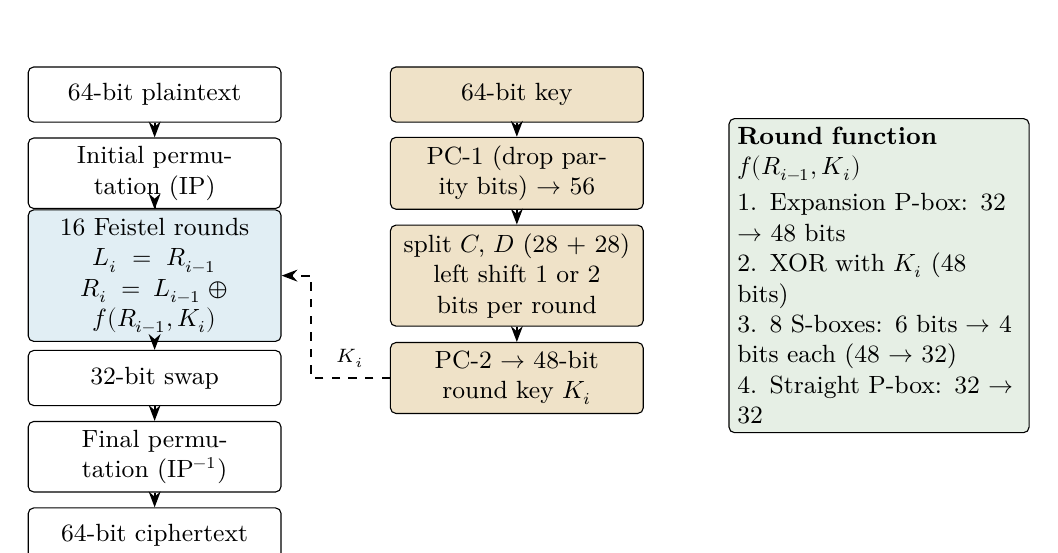
\begin{tikzpicture}[every node/.style={font=\scriptsize}, bx/.style={box,minimum width=30mm,text width=30mm}]
  % data path
  \node[bx] (p) at (0,0) {64-bit plaintext};
  \node[bx] (ip) at (0,-1) {Initial permutation (IP)};
  \node[bx,fill=cyan!10] (r) at (0,-2.3) {16 Feistel rounds\\$L_i = R_{i-1}$\\$R_i = L_{i-1} \oplus f(R_{i-1}, K_i)$};
  \node[bx] (sw) at (0,-3.6) {32-bit swap};
  \node[bx] (fp) at (0,-4.6) {Final permutation (IP$^{-1}$)};
  \node[bx] (c) at (0,-5.6) {64-bit ciphertext};
  \foreach \u/\v in {p/ip,ip/r,r/sw,sw/fp,fp/c} \draw[arr] (\u)--(\v);
  % key schedule
  \node[bx,fill=yellow!20] (k) at (4.6,0) {64-bit key};
  \node[bx,fill=yellow!20] (pc1) at (4.6,-1) {PC-1 (drop parity bits) $\to$ 56};
  \node[bx,fill=yellow!20] (sh) at (4.6,-2.3) {split $C$, $D$ (28 + 28)\\left shift 1 or 2 bits per round};
  \node[bx,fill=yellow!20] (pc2) at (4.6,-3.6) {PC-2 $\to$ 48-bit round key $K_i$};
  \foreach \u/\v in {k/pc1,pc1/sh,sh/pc2} \draw[arr] (\u)--(\v);
  \draw[arr,dashed] (pc2.west) -- node[above]{$K_i$} ++(-1.0,0) |- (r.east);
  % round function
  \node[box,fill=green!12,text width=36mm,align=left] (f) at (9.2,-2.3) {\textbf{Round function} $f(R_{i-1}, K_i)$\\[2pt]
    1. Expansion P-box: 32 $\to$ 48 bits\\2. XOR with $K_i$ (48 bits)\\3. 8 S-boxes: 6 bits $\to$ 4 bits each (48 $\to$ 32)\\4. Straight P-box: 32 $\to$ 32};
\end{tikzpicture}
\end{center}
\begin{itemize}
  \item \textbf{Feistel structure:} each round changes only one half and then swaps the halves. Decryption is the \emph{same} algorithm with the round keys used in reverse ($K_{16}, \dots, K_1$). $f$ need not be invertible.
  \item \textbf{Shifts:} 1 bit in rounds 1, 2, 9, 16; 2 bits in all the others (28 bits in total).
\end{itemize}
\begin{minipage}[t]{0.48\textwidth}\small
\textbf{S-box substitution (pseudocode)}\\
\ttfamily for i = 1 to 8:\\
\hspace*{1em}b = in[6i-5 .. 6i]\quad // 6 bits\\
\hspace*{1em}row = 2*b1 + b6\quad // outer bits\\
\hspace*{1em}col = b2b3b4b5\quad // inner 4 bits\\
\hspace*{1em}out[4i-3 .. 4i] = S[i][row][col]\\
return out\quad // 32 bits
\end{minipage}\hfill
\begin{minipage}[t]{0.48\textwidth}\small
\textbf{Key generation (pseudocode)}\\
\ttfamily K56 = PC1(K64)\\
C = K56[1..28]; D = K56[29..56]\\
for i = 1 to 16:\\
\hspace*{1em}s = (i in \{1,2,9,16\}) ? 1 : 2\\
\hspace*{1em}C = rotl(C, s); D = rotl(D, s)\\
\hspace*{1em}K[i] = PC2(C || D)\quad // 48 bits\\
return K[1..16]
\end{minipage}

\medskip
\textbf{Q7 (5).} \emph{Pseudocode for finding an inverse, and finding $23^{-1}$ in $\mathbb{Z}_{100}$.}
This is the \textbf{extended Euclidean algorithm} (pseudocode in the method box). Mr X's worry is real: an inverse exists only when $\gcd = 1$, and the same algorithm tells him so when it doesn't. Here $\gcd(100, 23) = 1$:
\begin{center}\small
\begin{tabular}{@{}cccccccc@{}}
\toprule
Iter. & $q$ & $r_1$ & $r_2$ & $r$ & $t_1$ & $t_2$ & $t$\\
\midrule
1 & 4 & 100 & 23 & 8 & 0 & 1 & $-4$\\
2 & 2 & 23 & 8 & \textbf{7} & 1 & $-4$ & 9\\
3 & 1 & 8 & 7 & 1 & $-4$ & 9 & $\mathbf{-13}$\\
4 & 7 & 7 & 1 & 0 & 9 & $-13$ & \textbf{100}\\
 & & \textbf{1} & 0 & & $\mathbf{-13}$ & 100 & \\
\bottomrule
\end{tabular}
\end{center}
\begin{enumerate}[leftmargin=1.5em]
  \item \textbf{4 iterations}.
  \item Remainder in iteration 2: $r = \mathbf{7}$.
  \item Coefficient in iteration 4: $t = \mathbf{100}$ (always $\pm n$ in the last step; a useful self-check).
  \item Inverse value in iteration 3: $t = -13$, which is the final answer: $23^{-1} \equiv -13 \equiv \mathbf{87} \pmod{100}$. Check: $23 \times 87 = 2001 = 20\cdot100 + 1$ \checkmark.
\end{enumerate}

% ================================================================
\subsection{Mid-Sem 2025--26, solved}

\textbf{Q1 (8).} \emph{One-time-pad Vigen\`ere; key stream 9 0 1 7 23 15 21 14 11 11 2 8 9.}
\begin{center}\small\setlength{\tabcolsep}{4pt}
\begin{tabular}{@{}l*{13}{c}@{}}
\toprule
Plain & s&e&n&d&m&o&r&e&m&o&n&e&y\\
$P$ & 18&4&13&3&12&14&17&4&12&14&13&4&24\\
Key & 9&0&1&7&23&15&21&14&11&11&2&8&9\\
$P{+}K$ & \hl{27}&4&14&10&\hl{35}&\hl{29}&\hl{38}&18&23&25&15&12&\hl{33}\\
mod 26 & 1&4&14&10&9&3&12&18&23&25&15&12&7\\
Cipher & \textbf{B}&\textbf{E}&\textbf{O}&\textbf{K}&\textbf{J}&\textbf{D}&\textbf{M}&\textbf{S}&\textbf{X}&\textbf{Z}&\textbf{P}&\textbf{M}&\textbf{H}\\
\bottomrule
\end{tabular}
\end{center}
(a) \textbf{\ttx{BEOKJDMSXZPMH}}.
(b) We need $K = (C - P) \bmod 26$ with $P$ = \ttx{cashnotneeded}:
\begin{center}\small\setlength{\tabcolsep}{4pt}
\begin{tabular}{@{}l*{13}{c}@{}}
\toprule
$C$ & B 1&E 4&O 14&K 10&J 9&D 3&M 12&S 18&X 23&Z 25&P 15&M 12&H 7\\
$P$ & c 2&a 0&s 18&h 7&n 13&o 14&t 19&n 13&e 4&e 4&d 3&e 4&d 3\\
$C - P$ & $-1$&4&$-4$&3&$-4$&$-11$&$-7$&5&19&21&12&8&4\\
Key & \textbf{25}&\textbf{4}&\textbf{22}&\textbf{3}&\textbf{22}&\textbf{15}&\textbf{19}&\textbf{5}&\textbf{19}&\textbf{21}&\textbf{12}&\textbf{8}&\textbf{4}\\
\bottomrule
\end{tabular}
\end{center}
Key stream: \textbf{25 4 22 3 22 15 19 5 19 21 12 8 4}. This is the point of the question: for \emph{any} ciphertext there is a key giving \emph{any} plaintext of the same length, which is why a one-time pad can't be broken (Section 13).

\textbf{Q2 (4).} \emph{Inverse of $x^7$ mod $x^8 + x^4 + x^3 + x + 1$.}
\begin{center}\small\setlength{\tabcolsep}{3pt}
\begin{tabular}{@{}lllllll@{}}
\toprule
$q$ & $r_1$ & $r_2$ & $r$ & $t_1$ & $t_2$ & $t$\\
\midrule
$x$ & $x^8{+}x^4{+}x^3{+}x{+}1$ & $x^7$ & $x^4{+}x^3{+}x{+}1$ & 0 & 1 & $x$\\
$x^3{+}x^2{+}x$ & $x^7$ & $x^4{+}x^3{+}x{+}1$ & $x$ & 1 & $x$ & $x^4{+}x^3{+}x^2{+}1$\\
$x^3{+}x^2{+}1$ & $x^4{+}x^3{+}x{+}1$ & $x$ & 1 & $x$ & $x^4{+}x^3{+}x^2{+}1$ & $x^7{+}x{+}1$\\
$x$ & $x$ & 1 & 0 & $x^4{+}x^3{+}x^2{+}1$ & $x^7{+}x{+}1$ & $m$\\
 & \textbf{1} & 0 & & $\mathbf{x^7{+}x{+}1}$ & & \\
\bottomrule
\end{tabular}
\end{center}
$(x^7)^{-1} = \mathbf{x^7 + x + 1}$ (byte \ttx{83}). (Row 2 detail: $x^7 \div (x^4{+}x^3{+}x{+}1)$ gives quotient $x^3{+}x^2{+}x$ and remainder $x$, all with XOR subtraction.)

\textbf{Q3 (4).} \emph{Playfair with the given key matrix: ``Insta Reels Pe Time Waste Na Kar'' (filler X, I/J together).}
\begin{center}\small
\begin{minipage}[c]{0.25\textwidth}\centering
\begin{tabular}{|*{5}{c|}}\hline L&A&R&K&S\\\hline P&U&B&C&D\\\hline E&F&G&H&I/J\\\hline M&N&O&Q&T\\\hline V&W&X&Y&Z\\\hline\end{tabular}
\end{minipage}
\begin{minipage}[c]{0.7\textwidth}
Digrams (\ttx{ee} in ``reels'' $\to$ \ttx{ex}, then re-pair; odd length, so \ttx{r} becomes \ttx{rx}):\\
\ttx{in st ar ex el sp et im ew as te na ka rx}\\[2pt]
\ttx{FT DZ RK GV MP LD IM ET FV RL MI WU SR BR}\\[2pt]
(rows: \ttx{ar}, \ttx{as}, \ttx{ka}; columns: \ttx{st}, \ttx{el}, \ttx{na}, \ttx{rx}; the rest are rectangles)
\end{minipage}
\end{center}
Ciphertext: \textbf{\ttx{FTDZRKGVMPLDIMETFVRLMIWUSRBR}}.
\emph{Trap:} in ``reels'' the \ttx{ee} lands inside one pair (\ttx{r e | e l} would be wrong). Pairing from the start gives \ttx{in st ar \underline{ee}}, so the filler goes in there.

\textbf{Q4 (6).} \emph{AES: (a) ShiftRows, (b) AddRoundKey.}\\
(a) Row $r$ is rotated \textbf{left by $r$ bytes} (row 0 unchanged):
\[
\begin{pmatrix}\mathtt{87}&\mathtt{F2}&\mathtt{4D}&\mathtt{97}\\\mathtt{EC}&\mathtt{6E}&\mathtt{4C}&\mathtt{90}\\\mathtt{4A}&\mathtt{C3}&\mathtt{46}&\mathtt{E7}\\\mathtt{8C}&\mathtt{D8}&\mathtt{95}&\mathtt{A6}\end{pmatrix}
\;\xrightarrow{\text{ShiftRows}}\;
\begin{pmatrix}\mathtt{87}&\mathtt{F2}&\mathtt{4D}&\mathtt{97}\\\mathtt{6E}&\mathtt{4C}&\mathtt{90}&\mathtt{EC}\\\mathtt{46}&\mathtt{E7}&\mathtt{4A}&\mathtt{C3}\\\mathtt{A6}&\mathtt{8C}&\mathtt{D8}&\mathtt{95}\end{pmatrix}
\]
(b) AddRoundKey $=$ \textbf{byte-wise XOR} of state and key. E.g.\ $\mathtt{47} \oplus \mathtt{AC}$: $\;0100\,0111 \oplus 1010\,1100 = 1110\,1011 = EB$.
\[
\begin{pmatrix}\mathtt{47}&\mathtt{40}&\mathtt{A3}&\mathtt{4C}\\\mathtt{37}&\mathtt{D4}&\mathtt{70}&\mathtt{9F}\\\mathtt{94}&\mathtt{E4}&\mathtt{3A}&\mathtt{42}\\\mathtt{ED}&\mathtt{A5}&\mathtt{A6}&\mathtt{BC}\end{pmatrix}
\oplus
\begin{pmatrix}\mathtt{AC}&\mathtt{19}&\mathtt{28}&\mathtt{57}\\\mathtt{77}&\mathtt{FA}&\mathtt{D1}&\mathtt{5C}\\\mathtt{66}&\mathtt{DC}&\mathtt{29}&\mathtt{00}\\\mathtt{F3}&\mathtt{21}&\mathtt{41}&\mathtt{6A}\end{pmatrix}
=
\begin{pmatrix}\boldsymbol{\mathtt{EB}}&\boldsymbol{\mathtt{59}}&\boldsymbol{\mathtt{8B}}&\boldsymbol{\mathtt{1B}}\\\boldsymbol{\mathtt{40}}&\boldsymbol{\mathtt{2E}}&\boldsymbol{\mathtt{A1}}&\boldsymbol{\mathtt{C3}}\\\boldsymbol{\mathtt{F2}}&\boldsymbol{\mathtt{38}}&\boldsymbol{\mathtt{13}}&\boldsymbol{\mathtt{42}}\\\boldsymbol{\mathtt{1E}}&\boldsymbol{\mathtt{84}}&\boldsymbol{\mathtt{E7}}&\boldsymbol{\mathtt{D6}}\end{pmatrix}
\]
Tip: XOR one hex digit at a time ($\mathtt4 \oplus \mathtt A = 0100 \oplus 1010 = 1110 = \mathtt E$, \;$\mathtt7 \oplus \mathtt C = 0111 \oplus 1100 = 1011 = \mathtt B$).

\textbf{Q5 (3).} \emph{Solve $19x + 13y = 20$.}
$\gcd(19, 13) = 1$, and $1 \mid 20$, so solutions exist. Euclid: $19 = 1\cdot13 + 6$, $13 = 2\cdot6 + 1$. Back-substitute:
$1 = 13 - 2\cdot6 = 13 - 2(19 - 13) = 3\cdot13 - 2\cdot19$, so $s = -2$, $t = 3$.
Times 20: $x_0 = -40$, $y_0 = 60$. General solution: $x = -40 + 13k$, $y = 60 - 19k$. Taking $k = 3$: \textbf{$x = -1$, $y = 3$}, so in general \textbf{$x = -1 + 13k$, $y = 3 - 19k$}.
Check: $19(-1) + 13(3) = -19 + 39 = 20$ \checkmark.

% ================================================================
\clearpage
\subsection{Mock Mid-Sem paper (same style), 90 minutes, 25 marks}
\emph{Precise answer with proper justification will be considered to get complete marks. Attempt all questions.}
\begin{center}\small
\begin{tabularx}{\textwidth}{|c|X|c|}
\hline
\textbf{Q} & & \textbf{Marks}\\\hline
1 & What is the maximum number of characters that change in the \emph{ciphertext} if a single plaintext character is changed, for: (a) Hill ($2\times2$) (b) Playfair (c) row--column transposition? (d) In the auto-key cipher (keyword length $m$), if \emph{one ciphertext character} is corrupted in transit, how many plaintext characters come out wrong after decryption? & 2\\\hline
2 & Using the Playfair cipher with the key ``MNNIT ALLAHABAD'' (I/J in one cell, filler X), encrypt ``Jazz night at the hall tomorrow''. & 4\\\hline
3 & Eve types ``abcdefghijkl'' on Alice's computer and the screen shows ``BDACFHEGJLIK''. Alice uses a keyed transposition cipher.
(a) What type of attack is this? (b) What is the key size? (c) Give the encryption and decryption keys. (d) Decrypt ``ETMEETMAONNO''. & 3\\\hline
4 & In GF$(2^8)$ find the inverse of $(x^6 + x^4 + x + 1)$ modulo $(x^8 + x^4 + x^3 + x + 1)$. Verify your answer. & 4\\\hline
5 & (i) In GF(11) find $7 \div 9$. (ii) Find $2^{90} \bmod 13$ and $1000^{999} \bmod 7$. (iii) Find, if they exist, $11^{-1} \bmod 26$, $26^{-1} \bmod 39$ and $17^{-1} \bmod 101$. & 3\\\hline
6 & Solve the linear Diophantine equations, or show there is no solution: (i) $24x + 138y = 18$ (ii) $15x + 21y = 7$. & 3\\\hline
7 & Using the extended Euclidean algorithm, find $47^{-1}$ in $\mathbb{Z}_{120}$. State (a) the number of iterations, (b) the remainder in iteration 2, (c) $t$ in iteration 3. (d) Does $46$ have an inverse in $\mathbb{Z}_{120}$? Justify. & 3\\\hline
8 & AES. State $S = \begin{pmatrix}\mathtt{19}&\mathtt{A0}&\mathtt{9A}&\mathtt{E9}\\\mathtt{3D}&\mathtt{F4}&\mathtt{C6}&\mathtt{F8}\\\mathtt{E3}&\mathtt{E2}&\mathtt{8D}&\mathtt{48}\\\mathtt{BE}&\mathtt{2B}&\mathtt{2A}&\mathtt{08}\end{pmatrix}$, round key $K = \begin{pmatrix}\mathtt{A0}&\mathtt{88}&\mathtt{23}&\mathtt{2A}\\\mathtt{FA}&\mathtt{54}&\mathtt{A3}&\mathtt{6C}\\\mathtt{FE}&\mathtt{2C}&\mathtt{39}&\mathtt{76}\\\mathtt{17}&\mathtt{B1}&\mathtt{39}&\mathtt{05}\end{pmatrix}$.
(a) Apply ShiftRows to $S$. (b) Apply AddRoundKey with $K$ to your result from (a) (skip MixColumns here). & 3\\\hline
\end{tabularx}
\end{center}

\clearpage
\subsection{Mock paper: model answers}

\textbf{M1.} (a) \textbf{2}: one block of 2 letters; both can change. (b) Usually 2 (one digram), but the \textbf{maximum is every remaining character}: changing a letter can create or remove a doubled pair (e.g.\ ``bal\underline{k}'' $\to$ ``bal\underline{l}''), which adds or removes a filler and shifts every later digram. (c) \textbf{1}: transposition only moves letters, so exactly one ciphertext letter (somewhere else) changes. (d) The wrong $P_i$ is then used as the key for $P_{i+m}$, which is used for $P_{i+2m}$, and so on: the error \textbf{propagates to every $m$-th character until the end}.

\textbf{M2.} Key without repeats: M N I T A L H B D, then the rest.
\begin{center}\small
\begin{minipage}[c]{0.25\textwidth}\centering
\begin{tabular}{|*{5}{c|}}\hline M&N&I/J&T&A\\\hline L&H&B&D&C\\\hline E&F&G&K&O\\\hline P&Q&R&S&U\\\hline V&W&X&Y&Z\\\hline\end{tabular}
\end{minipage}
\begin{minipage}[c]{0.7\textwidth}
\ttx{jazznightatthehalltomorrow}, J $\to$ I. Only \ttx{zz} lands in one pair: \ttx{zx}. The \ttx{tt}, \ttx{ll} and \ttx{rr} are each split across pairs (traps!). Odd length, so \ttx{w} becomes \ttx{wx}:\\
\ttx{ia zx zn ig ht at th eh al lt om or ro wx}\\[2pt]
\ttx{TM VY WA BR DN MA ND FL MC DM EA GU UG XY}
\end{minipage}
\end{center}
Ciphertext: \textbf{\ttx{TMVYWABRDNMANDFLMCDMEAGUUGXY}}. (Note \ttx{or}$\to$\ttx{GU} and \ttx{ro}$\to$\ttx{UG}: reversed pairs give reversed output.)

\textbf{M3.} (a) \textbf{Chosen-plaintext}. (b) The pattern repeats every 4 (\ttx{abcd}$\to$\ttx{BDAC}, \ttx{efgh}$\to$\ttx{FHEG}), so the \textbf{key size is 4}.
(c) Encryption key \textbf{(2 4 1 3)}: output position $j$ takes input position key[$j$]. Decryption key = inverse \textbf{(3 1 4 2)}.
(d) Blocks \ttx{ETME | ETMA | ONNO}, each rearranged as positions 3, 1, 4, 2: \textbf{meet me at noon}.

\textbf{M4.} Table ($m = x^8{+}x^4{+}x^3{+}x{+}1$, $b = x^6{+}x^4{+}x{+}1$):
\begin{center}\small\setlength{\tabcolsep}{3pt}
\begin{tabular}{@{}lllllll@{}}
\toprule
$q$ & $r_1$ & $r_2$ & $r$ & $t_1$ & $t_2$ & $t$\\
\midrule
$x^2{+}1$ & $m$ & $x^6{+}x^4{+}x{+}1$ & $x^2$ & 0 & 1 & $x^2{+}1$\\
$x^4{+}x^2$ & $x^6{+}x^4{+}x{+}1$ & $x^2$ & $x{+}1$ & 1 & $x^2{+}1$ & $x^6{+}x^2{+}1$\\
$x{+}1$ & $x^2$ & $x{+}1$ & 1 & $x^2{+}1$ & $x^6{+}x^2{+}1$ & $x^7{+}x^6{+}x^3{+}x$\\
$x{+}1$ & $x{+}1$ & 1 & 0 & $x^6{+}x^2{+}1$ & $x^7{+}x^6{+}x^3{+}x$ & $m$\\
 & \textbf{1} & 0 & & $\mathbf{x^7{+}x^6{+}x^3{+}x}$ & & \\
\bottomrule
\end{tabular}
\end{center}
Inverse $= \mathbf{x^7 + x^6 + x^3 + x}$ (byte \ttx{CA}; i.e.\ $\{53\}^{-1} = \{CA\}$, the standard AES example).\\
Verified: $(x^6{+}x^4{+}x{+}1)(x^7{+}x^6{+}x^3{+}x) \bmod m = 1$.

\textbf{M5.} (i) $9^{-1} \bmod 11 = 5$ ($45 = 4\cdot11 + 1$), so $7 \div 9 = 7 \cdot 5 = 35 \equiv \mathbf{2}$.
(ii) Fermat: $2^{12} \equiv 1 \pmod{13}$ and $90 = 7\cdot12 + 6$, so $2^{90} \equiv 2^6 = 64 \equiv \mathbf{12}$. \;$1000 = 142\cdot7 + 6 \equiv -1$, so $(-1)^{999} = -1 \equiv \mathbf{6}$.
(iii) $11^{-1} \bmod 26 = \mathbf{19}$ ($209 = 8\cdot26 + 1$). $26^{-1} \bmod 39$: $\gcd(26, 39) = 13$, so it \textbf{does not exist}. $17^{-1} \bmod 101 = \mathbf{6}$ ($102 = 101 + 1$).

\textbf{M6.} (i) $\gcd(24, 138) = 6$ and $6 \mid 18$, so solutions exist. Divide by 6: $4x + 23y = 3$. Since $4\cdot6 + 23\cdot(-1) = 1$, times 3 gives $x_0 = 18$, $y_0 = -3$.
General: $x = 18 + 23k$, $y = -3 - 4k$; with $k = -1$: \textbf{$x = -5 + 23k$, $y = 1 - 4k$}. Check: $24(-5) + 138(1) = 18$ \checkmark.
(ii) $\gcd(15, 21) = 3$, and $3 \nmid 7$: \textbf{no solution}. (The left side is always a multiple of 3.)

\textbf{M7.}
\begin{center}\small
\begin{tabular}{@{}cccccccc@{}}
\toprule
Iter. & $q$ & $r_1$ & $r_2$ & $r$ & $t_1$ & $t_2$ & $t$\\
\midrule
1 & 2 & 120 & 47 & 26 & 0 & 1 & $-2$\\
2 & 1 & 47 & 26 & \textbf{21} & 1 & $-2$ & 3\\
3 & 1 & 26 & 21 & 5 & $-2$ & 3 & $\mathbf{-5}$\\
4 & 4 & 21 & 5 & 1 & 3 & $-5$ & 23\\
5 & 5 & 5 & 1 & 0 & $-5$ & 23 & $-120$\\
 & & \textbf{1} & 0 & & \textbf{23} & & \\
\bottomrule
\end{tabular}
\end{center}
(a) \textbf{5 iterations}; (b) \textbf{21}; (c) $\mathbf{-5}$. \;$47^{-1} = \mathbf{23}$ (check: $47 \times 23 = 1081 = 9\cdot120 + 1$ \checkmark).
(d) \textbf{No}: $\gcd(46, 120) = 2 \ne 1$ (both even), so $46x$ is always even mod 120 and can never be 1.

\textbf{M8.} (a) $\begin{pmatrix}\mathtt{19}&\mathtt{A0}&\mathtt{9A}&\mathtt{E9}\\\mathtt{F4}&\mathtt{C6}&\mathtt{F8}&\mathtt{3D}\\\mathtt{8D}&\mathtt{48}&\mathtt{E3}&\mathtt{E2}\\\mathtt{08}&\mathtt{BE}&\mathtt{2B}&\mathtt{2A}\end{pmatrix}$ \quad
(b) XOR with $K$: $\begin{pmatrix}\boldsymbol{\mathtt{B9}}&\boldsymbol{\mathtt{28}}&\boldsymbol{\mathtt{B9}}&\boldsymbol{\mathtt{C3}}\\\boldsymbol{\mathtt{0E}}&\boldsymbol{\mathtt{92}}&\boldsymbol{\mathtt{5B}}&\boldsymbol{\mathtt{51}}\\\boldsymbol{\mathtt{73}}&\boldsymbol{\mathtt{64}}&\boldsymbol{\mathtt{DA}}&\boldsymbol{\mathtt{94}}\\\boldsymbol{\mathtt{1F}}&\boldsymbol{\mathtt{0F}}&\boldsymbol{\mathtt{12}}&\boldsymbol{\mathtt{2F}}\end{pmatrix}$
\;(e.g.\ $\mathtt{19} \oplus \mathtt{A0} = 0001\,1001 \oplus 1010\,0000 = 1011\,1001 = \mathtt{B9}$).

% Exam-pattern drill bank: questions written in the MNNIT CSN15403 mid-sem style, grouped by question type
\clearpage
\section{Exam-Pattern Drill Bank}\label{sec:drill}
Every question type that appeared in the 2024--25 and 2025--26 papers, several times over, with new numbers.
Do each group until the method is automatic. Marks follow the papers. Answers are in Section~\ref{sec:drillans}.

\newcounter{dq}
\newcommand{\dq}[1]{\refstepcounter{dq}\par\medskip\noindent\textbf{E\thedq.} \emph{[#1]}\ }

\subsection*{Type 1: cipher behaviour and attack types (2--3 marks)}
\dq{2} What is the maximum number of characters that change in the ciphertext if a single plaintext character is changed? (a) one-time pad (b) Hill cipher with a $3\times3$ key (c) keyed transposition (d) auto-key ($k_1 = k$, $k_i = P_{i-1}$).

\dq{2} A single \emph{ciphertext} character is corrupted in transit. How many plaintext characters are wrong after decryption? (a) Vigen\`ere (b) Hill ($2\times2$) (c) auto-key ($k_i = P_{i-1}$) (d) Playfair.

\dq{2} Name the attack: (a) Eve only listens to the channel. (b) Eve finds an old printout with a plaintext and its ciphertext. (c) Eve borrows Alice's encryption device for an hour. (d) Eve tricks Bob into decrypting a ciphertext she made up.

\dq{3} Eve uses Alice's computer, types ``abcdefghijkl'' and sees ``DFACEBJLGIKH''. Alice uses a keyed transposition cipher.
(a) What type of attack is this? (b) What is the key size? (c) Find the encryption and decryption keys. (d) Decrypt ``AKATCTANADWT''.

\dq{2} Encrypt ``enemy attacks tonight'' with the keyed transposition key (3 1 4 5 2), padding with ``z''.

\subsection*{Type 2: Playfair (3--4 marks)}
\dq{4} Use the Playfair cipher to encipher ``We meet at the bridge at midnight Jack''. The key is made by filling the first rows with ``CRYPTOGRAPHY'' and the rest with the remaining alphabet (I/J together, filler X).

\dq{3} Encrypt ``Balloon pops at noon'' with this key matrix:
\begin{center}\small\ttfamily
\begin{tabular}{ccccc}K&E&Y&W&O\\R&D&A&B&C\\F&G&H&I/J&L\\M&N&P&Q&S\\T&U&V&X&Z\end{tabular}
\end{center}

\dq{3} The Playfair key is ``SECURITY''. Decrypt \ttx{DAFSAFCFPMHSLGCSAFRTSBFHUV}.

\subsection*{Type 3: GF$(2^8)$ arithmetic (4 marks)}
For all of these, $m(x) = x^8 + x^4 + x^3 + x + 1$.

\dq{4} Find the multiplicative inverse of $x^2$ in GF$(2^8)$ mod $m(x)$.

\dq{4} Find the multiplicative inverse of $(x^3 + 1)$ in GF$(2^8)$ mod $m(x)$.

\dq{4} Find the multiplicative inverse of $x^4$ in GF$(2^8)$ mod $m(x)$.

\dq{4} Find the multiplicative inverse of $x^6$ in GF$(2^8)$ mod $m(x)$.

\dq{3} In GF$(2^8)$: (a) add $(x^6 + x^4 + x^2 + x + 1)$ and $(x^7 + x + 1)$; (b) multiply them mod $m(x)$.

\subsection*{Type 4: GF$(p)$, modular exponentiation, inverses (3 marks)}
\dq{3} (i) In GF(13) find $4 \div 7$, and in GF(17) find $3 \div 5$.
(ii) Find $999^{999} \bmod 10$, $7^{1000} \bmod 13$ and $1234^{4321} \bmod 5$.
(iii) Find, if they exist, $13^{-1} \bmod 47$, $12^{-1} \bmod 30$ and $5^{-1} \bmod 28$.

\dq{3} Find $777^{333} \bmod 7$, $2^{1000} \bmod 7$, $11^{500} \bmod 12$ and $46^{47} \bmod 47$.

\subsection*{Type 5: extended Euclidean algorithm (5 marks)}
\dq{5} Find $17^{-1}$ in $\mathbb{Z}_{43}$ with the extended Euclidean algorithm. State the number of iterations, the remainder in iteration 3, and $t$ in iteration 2.

\dq{5} Mr X wants $38^{-1}$ in $\mathbb{Z}_{180}$. Run the extended Euclidean algorithm and explain what the final row tells him. Which elements of $\{36, 37, 38, 39\}$ \emph{do} have inverses in $\mathbb{Z}_{180}$?

\dq{5} Find $550^{-1} \bmod 1769$. How many iterations are needed? Comment on the answer.

\subsection*{Type 6: linear Diophantine equations (3 marks)}
\dq{3} Solve, or show there is no solution: (i) $21x + 14y = 35$ \quad (ii) $40x + 15y = 110$ \quad (iii) $12x + 18y = 25$.

\dq{3} A shop sells pens for Rs.\,19 and notebooks for Rs.\,13. A student spends exactly Rs.\,220. How many of each did they buy? Is the answer unique?

\subsection*{Type 7: one-time pad / Vigen\`ere with a key stream (8 marks)}
\dq{8} One-time-pad Vigen\`ere: each plaintext letter is shifted by the next number of the key stream.
(a) Encrypt ``meetmeatnoon'' with the key stream 3 19 5 0 24 11 7 2 14 9 25 8.
(b) Using your ciphertext, find a key stream that makes it decrypt to ``holdposition''.
(c) Why does (b) show that Eve can't break this cipher by brute force?

\dq{3} Encrypt ``polyalphabetic'' with the Vigen\`ere keyword ``LEMON''.

\subsection*{Type 8: AES state operations (6 marks)}
\dq{6} AES state (rows) $S = \begin{pmatrix}\mathtt{32}&\mathtt{88}&\mathtt{31}&\mathtt{E0}\\\mathtt{43}&\mathtt{5A}&\mathtt{31}&\mathtt{37}\\\mathtt{F6}&\mathtt{30}&\mathtt{98}&\mathtt{07}\\\mathtt{A8}&\mathtt{8D}&\mathtt{A2}&\mathtt{34}\end{pmatrix}$, key $K = \begin{pmatrix}\mathtt{2B}&\mathtt{28}&\mathtt{AB}&\mathtt{09}\\\mathtt{7E}&\mathtt{AE}&\mathtt{F7}&\mathtt{CF}\\\mathtt{15}&\mathtt{D2}&\mathtt{15}&\mathtt{4F}\\\mathtt{16}&\mathtt{A6}&\mathtt{88}&\mathtt{3C}\end{pmatrix}$.
(a) Apply ShiftRows to $S$. (b) Apply AddRoundKey to $S$ (the original) with $K$.

\dq{3} After ShiftRows the state is $\begin{pmatrix}\mathtt{D4}&\mathtt{E0}&\mathtt{B8}&\mathtt{1E}\\\mathtt{27}&\mathtt{BF}&\mathtt{B4}&\mathtt{41}\\\mathtt{11}&\mathtt{98}&\mathtt{5D}&\mathtt{52}\\\mathtt{AE}&\mathtt{F1}&\mathtt{E5}&\mathtt{30}\end{pmatrix}$. What was it before ShiftRows?

\dq{3} $\bigstar$ (MixColumns, one byte.) A state column is $(\mathtt{87}, \mathtt{6E}, \mathtt{46}, \mathtt{A6})$. Compute the first byte of its MixColumns output, $\mathtt{02}\cdot\mathtt{87} \oplus \mathtt{03}\cdot\mathtt{6E} \oplus \mathtt{46} \oplus \mathtt{A6}$, in GF$(2^8)$.

\subsection*{Type 9: DES (5 marks)}
\dq{2} DES S-box $S_1$ (below). Find the output for the 6-bit inputs (a) \ttx{100011} (b) \ttx{011011} (c) \ttx{110110}.
\begin{center}\scriptsize\setlength{\tabcolsep}{2.5pt}
\begin{tabular}{c|*{16}{c}}
$S_1$ & 0&1&2&3&4&5&6&7&8&9&10&11&12&13&14&15\\\hline
0 & 14&4&13&1&2&15&11&8&3&10&6&12&5&9&0&7\\
1 & 0&15&7&4&14&2&13&1&10&6&12&11&9&5&3&8\\
2 & 4&1&14&8&13&6&2&11&15&12&9&7&3&10&5&0\\
3 & 15&12&8&2&4&9&1&7&5&11&3&14&10&0&6&13
\end{tabular}
\end{center}

\dq{3} DES key schedule. (a) By how many bits in total have $C$ and $D$ been rotated after rounds 2, 9 and 16? (b) Why is the total after round 16 important? (c) How many bits does PC-1 discard, and why?

\dq{5} Explain with a diagram why a Feistel cipher can decrypt with the \emph{same} round function even if $f$ is not invertible. Given one round's output $(L_1, R_1)$ and $K_1$, write $L_0$ and $R_0$.


\subsection*{Type 10: Fermat, Euler, primitive roots (3--4 marks)}
\dq{3} Using Fermat's little theorem, find (i) $6^{10} \bmod 11$ (ii) $3^{12} \bmod 11$ (iii) $2^{-1} \bmod 13$ (iv) $7^{-1} \bmod 19$.

\dq{4} Using Euler's theorem, find the multiplicative inverses: (i) $3^{-1} \bmod 20$ (ii) $7^{-1} \bmod 15$ (iii) $8^{-1} \bmod 77$ (iv) $60^{-1} \bmod 187$ (v) $71^{-1} \bmod 100$.

\dq{3} Find (i) $7^{222} \bmod 11$ (ii) $4^{532} \bmod 11$ (iii) $11^{2024} \bmod 35$.

\dq{4} (i) Show that 3 is a primitive root of 17. (ii) Find all primitive roots of 11. (iii) How many primitive roots does 23 have? Given that 5 is one, find another without building a table.

\dq{3} Find the order of every element of $\mathbb{Z}_7^*$ and identify its primitive roots. Does $\mathbb{Z}_8^*$ have a primitive root? Justify.

\dq{3} Evaluate, stating whether Fermat's theorem applies: (i) $12^{16} \bmod 17$ (ii) $17^{16} \bmod 17$ (iii) $2^{14} \bmod 15$: what does this tell you about 15? (iv) $2^{340} \bmod 341$ turns out to be 1. Is 341 prime?

% ===============================================================
\clearpage
\subsection{Drill bank: model answers}\label{sec:drillans}
\setcounter{dq}{0}
\newcommand{\da}{\refstepcounter{dq}\par\medskip\noindent\textbf{E\thedq.}\ }

\da (a) \textbf{1} (b) \textbf{3}: the whole block can change (c) \textbf{1}: letters only move, so one letter (at a new position) changes (d) \textbf{2}: $C_i$, and $C_{i+1}$ because $P_i$ is the key for the next letter.

\da (a) \textbf{1} (b) \textbf{2}: the whole block decrypts wrongly (c) \textbf{every character from there on}: wrong $P_i$ becomes the key for $P_{i+1}$, which is then wrong, and so on (d) \textbf{2}: one digram.

\da (a) ciphertext-only (b) known-plaintext (c) chosen-plaintext (d) chosen-ciphertext.

\da (a) \textbf{Chosen-plaintext}. (b) \ttx{abcdef}$\to$\ttx{DFACEB} and \ttx{ghijkl}$\to$\ttx{JLGIKH}: the same pattern, so the \textbf{key size is 6}. (It can't be 3: the first output letter, \ttx{d}, comes from outside \ttx{abc}.)
(c) Encryption key \textbf{(4 6 1 3 5 2)}: output $j$ takes input key[$j$]. Decryption key = inverse \textbf{(3 6 4 1 5 2)}.
(d) Blocks \ttx{AKATCT | ANADWT}, taking positions 3, 6, 4, 1, 5, 2 of each: \textbf{attack at dawn}.

\da 19 letters, padded to 20 with one \ttx{z}, in blocks of 5: \ttx{enemy}, \ttx{attac}, \ttx{kston}, \ttx{ightz}. Each block is output as positions 3, 1, 4, 5, 2:
\ttx{enemy}$\to$\ttx{EEMYN}, \ttx{attac}$\to$\ttx{TAACT}, \ttx{kston}$\to$\ttx{TKONS}, \ttx{ightz}$\to$\ttx{HITZG}. Answer: \textbf{\ttx{EEMYNTAACTTKONSHITZG}} (Forouzan's own example).

\da Matrix: \ttx{C R Y P T / O G A H B / D E F I K / L M N Q S / U V W X Z}.
Text: \ttx{we meet at the bridge at midnight iack} (J$\to$I). The \ttx{ee} and \ttx{tt} split across pairs, so no filler is needed; the length is odd, so pad with \ttx{x}:
\ttx{we me et at th eb ri dg ea tm id ni gh ti ac kx}\\
$\to$ \ttx{VF VM KR BY PB KG PE EO FG RS KE QF AB PK OY IZ} \;(\ttx{me}: column; \ttx{id}, \ttx{gh}: rows).\\
Answer: \textbf{\ttx{VFVMKRBYPBKGPEEOFGRSKEQFABPKOYIZ}}.

\da \ttx{balloonpopsatnoon}: \ttx{ba}, then \ttx{ll} is a double, so \ttx{lx} and re-pair: \ttx{lo on po ps at no on}. Even length now, so no padding.
\ttx{ba lx lo on po ps at no on} $\to$ \textbf{\ttx{CB IZ SC ES SY QM RV SE ES}}.
\emph{Trap:} after \ttx{lx}, the \ttx{oo} falls across \ttx{lo | on}, so no second filler is needed.

\da Matrix: \ttx{S E C U R / I T Y A B / D F G H K / L M N O P / Q V W X Z}. Decrypt (row: left; column: up; rectangle: same rule):
\ttx{hi de th eg ol du nd er th eb ri dg ex} $\to$ remove the final filler: \textbf{``hide the gold under the bridge''}.

\da $q$, $r_1$, $r_2$, $r$, $t_1$, $t_2$, $t$:
\begin{center}\small\setlength{\tabcolsep}{3pt}
\begin{tabular}{@{}lllllll@{}}
\toprule
$x^6{+}x^2{+}x$ & $m$ & $x^2$ & $x{+}1$ & 0 & 1 & $x^6{+}x^2{+}x$\\
$x{+}1$ & $x^2$ & $x{+}1$ & 1 & 1 & $x^6{+}x^2{+}x$ & $x^7{+}x^6{+}x^3{+}x{+}1$\\
$x{+}1$ & $x{+}1$ & 1 & 0 & $x^6{+}x^2{+}x$ & $x^7{+}x^6{+}x^3{+}x{+}1$ & $m$\\
\bottomrule
\end{tabular}
\end{center}
$(x^2)^{-1} = \mathbf{x^7 + x^6 + x^3 + x + 1}$ (\ttx{CB}). Row 1: $m \div x^2$ gives $q = x^6{+}x^2{+}x$, $r = x{+}1$.

\da
\begin{center}\small\setlength{\tabcolsep}{3pt}
\begin{tabular}{@{}lllllll@{}}
\toprule
$x^5{+}x^2{+}x{+}1$ & $m$ & $x^3{+}1$ & $x^2$ & 0 & 1 & $x^5{+}x^2{+}x{+}1$\\
$x$ & $x^3{+}1$ & $x^2$ & 1 & 1 & $x^5{+}x^2{+}x{+}1$ & $x^6{+}x^3{+}x^2{+}x{+}1$\\
$x^2$ & $x^2$ & 1 & 0 & $x^5{+}x^2{+}x{+}1$ & $x^6{+}x^3{+}x^2{+}x{+}1$ & $m$\\
\bottomrule
\end{tabular}
\end{center}
$(x^3{+}1)^{-1} = \mathbf{x^6 + x^3 + x^2 + x + 1}$ (\ttx{4F}).

\da
\begin{center}\small\setlength{\tabcolsep}{3pt}
\begin{tabular}{@{}lllllll@{}}
\toprule
$x^4{+}1$ & $m$ & $x^4$ & $x^3{+}x{+}1$ & 0 & 1 & $x^4{+}1$\\
$x$ & $x^4$ & $x^3{+}x{+}1$ & $x^2{+}x$ & 1 & $x^4{+}1$ & $x^5{+}x{+}1$\\
$x{+}1$ & $x^3{+}x{+}1$ & $x^2{+}x$ & 1 & $x^4{+}1$ & $x^5{+}x{+}1$ & $x^6{+}x^5{+}x^4{+}x^2$\\
$x^2{+}x$ & $x^2{+}x$ & 1 & 0 & $x^5{+}x{+}1$ & $x^6{+}x^5{+}x^4{+}x^2$ & $m$\\
\bottomrule
\end{tabular}
\end{center}
$(x^4)^{-1} = \mathbf{x^6 + x^5 + x^4 + x^2}$ (\ttx{74}).

\da
\begin{center}\small\setlength{\tabcolsep}{3pt}
\begin{tabular}{@{}lllllll@{}}
\toprule
$x^2$ & $m$ & $x^6$ & $x^4{+}x^3{+}x{+}1$ & 0 & 1 & $x^2$\\
$x^2{+}x{+}1$ & $x^6$ & $x^4{+}x^3{+}x{+}1$ & 1 & 1 & $x^2$ & $x^4{+}x^3{+}x^2{+}1$\\
$x^4{+}x^3{+}x{+}1$ & $x^4{+}x^3{+}x{+}1$ & 1 & 0 & $x^2$ & $x^4{+}x^3{+}x^2{+}1$ & $m$\\
\bottomrule
\end{tabular}
\end{center}
$(x^6)^{-1} = \mathbf{x^4 + x^3 + x^2 + 1}$ (\ttx{1D}).
\emph{Pattern:} in the first row, $x^k \cdot q$ is always the top part of $m$; the remainder is the low part $x^4{+}x^3{+}x{+}1$ whenever $k \ge 5$.

\da (a) Addition is XOR, so equal terms cancel: $(x^6{+}x^4{+}x^2{+}x{+}1) + (x^7{+}x{+}1) = \mathbf{x^7 + x^6 + x^4 + x^2}$ (\ttx{57} $\oplus$ \ttx{83} $=$ \ttx{D4}).
(b) The product is $x^{13}{+}x^{11}{+}x^9{+}x^8{+}x^6{+}x^5{+}x^4{+}x^3{+}1$. Reduce with $x^8 = x^4{+}x^3{+}x{+}1$ (and $x^9, \dots, x^{13}$ likewise) to get $\mathbf{x^7 + x^6 + 1}$ (\ttx{C1}). This is Stallings' worked example $\{57\}\cdot\{83\} = \{C1\}$.

\da (i) $7^{-1} \bmod 13 = 2$ ($14 \equiv 1$), so $4 \div 7 = 8$. \;$5^{-1} \bmod 17 = 7$ ($35 \equiv 1$), so $3 \div 5 = 21 \equiv 4$. Answers: \textbf{8, 4}.
(ii) $999 \equiv -1 \pmod{10}$, odd power: $\mathbf{9}$. \;$7^{12} \equiv 1 \pmod{13}$ and $1000 = 83\cdot12 + 4$: $7^4 = 2401 \equiv \mathbf{9}$. \;$1234 \equiv -1 \pmod 5$, odd power: $\mathbf{4}$.
(iii) $13^{-1} \bmod 47 = \mathbf{29}$ ($377 = 8\cdot47 + 1$). $12^{-1} \bmod 30$: $\gcd = 6$, \textbf{does not exist}. $5^{-1} \bmod 28 = \mathbf{17}$ ($85 = 3\cdot28 + 1$).

\da $777 = 111\cdot7 \equiv 0$, so the answer is $\mathbf{0}$. (\emph{Trap:} Fermat needs $\gcd(a, p) = 1$; you can't conclude ``$\equiv 1$''.)
$2^3 \equiv 1 \pmod 7$ and $1000 = 333\cdot3 + 1$, so the answer is $\mathbf{2}$. \;$11 \equiv -1 \pmod{12}$, even power: $\mathbf{1}$. \;$46 \equiv -1 \pmod{47}$, odd power: $\mathbf{46}$ (or by Fermat, $a^p \equiv a$).

\da
\begin{center}\small
\begin{tabular}{@{}cccccccc@{}}
\toprule Iter. & $q$ & $r_1$ & $r_2$ & $r$ & $t_1$ & $t_2$ & $t$\\\midrule
1 & 2 & 43 & 17 & 9 & 0 & 1 & $-2$\\
2 & 1 & 17 & 9 & 8 & 1 & $-2$ & $\mathbf{3}$\\
3 & 1 & 9 & 8 & \textbf{1} & $-2$ & 3 & $-5$\\
4 & 8 & 8 & 1 & 0 & 3 & $-5$ & 43\\
 & & 1 & 0 & & $-5$ & & \\\bottomrule
\end{tabular}
\end{center}
\textbf{4 iterations}; remainder in iteration 3 $= \mathbf{1}$; $t$ in iteration 2 $= \mathbf{3}$. \;$17^{-1} = -5 \equiv \mathbf{38}$ (check: $17 \cdot 38 = 646 = 15\cdot43 + 1$ \checkmark).

\da Table: $q = 4, 1, 2, 1, 4$; remainders $28, 10, 8, 2, 0$. The final row has $r_1 = \mathbf{2}$, not 1, so $\gcd(180, 38) = 2$ and \textbf{38 has no inverse} in $\mathbb{Z}_{180}$. The algorithm itself detects the failure.
$180 = 2^2\cdot3^2\cdot5$, so only numbers co-prime to 2, 3 and 5 have inverses: 36 (no), \textbf{37 (yes)}, 38 (no), 39 (no, divisible by 3).

\da Quotients $3, 4, 1, 1, 1, 1, 1, 4, 3$, so \textbf{9 iterations}. The final $t_1 = \mathbf{550}$: $550^{-1} \equiv 550 \pmod{1769}$. \emph{550 is its own inverse}: $550^2 = 302500 = 171\cdot1769 + 1$. (Stallings' example; a surprising answer worth checking rather than doubting.)

\da (i) $\gcd(21, 14) = 7$ and $7 \mid 35$. Divide by 7: $3x + 2y = 5$. Here $x = 1, y = 1$ works, so \textbf{$x = 1 + 2k$, $y = 1 - 3k$}.
(ii) $\gcd(40, 15) = 5$ and $5 \mid 110$. Divide: $8x + 3y = 22$; $x = 2, y = 2$ works, so \textbf{$x = 2 + 3k$, $y = 2 - 8k$}.
(iii) $\gcd(12, 18) = 6$ and $6 \nmid 25$: \textbf{no solution}.

\da $19x + 13y = 220$, $\gcd = 1$. From Euclid, $19(-2) + 13(3) = 1$, so $x_0 = -440$, $y_0 = 660$, and in general $x = -440 + 13k$, $y = 660 - 19k$.
Both must be $\ge 0$: $k \ge 33.9$ and $k \le 34.7$, so $k = 34$: \textbf{2 pens and 14 notebooks} ($38 + 182 = 220$). The non-negative answer is \textbf{unique}.

\da (a) $P + K$: $12{+}3,\allowbreak\ 4{+}19,\allowbreak\ 4{+}5,\allowbreak\ 19{+}0,\allowbreak\ 12{+}24,\allowbreak\ 4{+}11,\allowbreak\ 0{+}7,\allowbreak\ 19{+}2,\allowbreak\ 13{+}14,\allowbreak\ 14{+}9,\allowbreak\ 14{+}25,\allowbreak\ 13{+}8 = 15,\allowbreak\ 23,\allowbreak\ 9,\allowbreak\ 19,\allowbreak\ 36,\allowbreak\ 15,\allowbreak\ 7,\allowbreak\ 21,\allowbreak\ 27,\allowbreak\ 23,\allowbreak\ 39,\allowbreak\ 21$. Mod 26: \textbf{\ttx{PXJTKPHVBXNV}}.
(b) $K = C - P \pmod{26}$ with $P$ = \ttx{holdposition}: \textbf{8 9 24 16 21 1 15 13 8 15 25 8}.
(c) Every 12-letter message is reachable from this ciphertext with some key, and every key is equally likely, so the ciphertext gives no information (perfect secrecy).

\da Key \ttx{LEMONLEMONLEMO}: \textbf{\ttx{ASXMNWTTOOPXUQ}}.

\da (a) Rotate row $r$ left by $r$: $\begin{pmatrix}\mathtt{32}&\mathtt{88}&\mathtt{31}&\mathtt{E0}\\\mathtt{5A}&\mathtt{31}&\mathtt{37}&\mathtt{43}\\\mathtt{98}&\mathtt{07}&\mathtt{F6}&\mathtt{30}\\\mathtt{34}&\mathtt{A8}&\mathtt{8D}&\mathtt{A2}\end{pmatrix}$.
(b) XOR with $K$: $\begin{pmatrix}\mathtt{19}&\mathtt{A0}&\mathtt{9A}&\mathtt{E9}\\\mathtt{3D}&\mathtt{F4}&\mathtt{C6}&\mathtt{F8}\\\mathtt{E3}&\mathtt{E2}&\mathtt{8D}&\mathtt{48}\\\mathtt{BE}&\mathtt{2B}&\mathtt{2A}&\mathtt{08}\end{pmatrix}$ (e.g.\ $\mathtt{32}\oplus\mathtt{2B} = 0011\,0010 \oplus 0010\,1011 = 0001\,1001 = \mathtt{19}$).
These are the official AES (FIPS-197) test values: the initial AddRoundKey of round 0.

\da InvShiftRows rotates row $r$ \textbf{right} by $r$: $\begin{pmatrix}\mathtt{D4}&\mathtt{E0}&\mathtt{B8}&\mathtt{1E}\\\mathtt{BF}&\mathtt{B4}&\mathtt{41}&\mathtt{27}\\\mathtt{5D}&\mathtt{52}&\mathtt{11}&\mathtt{98}\\\mathtt{30}&\mathtt{AE}&\mathtt{F1}&\mathtt{E5}\end{pmatrix}$.

\da $\mathtt{02}\cdot b$ (``xtime''): shift left 1; if a 1 falls off the top, XOR with $\mathtt{1B}$. \;$\mathtt{03}\cdot b = (\mathtt{02}\cdot b) \oplus b$.
$\mathtt{02}\cdot\mathtt{87}$: $1000\,0111 \to 0000\,1110 \oplus 0001\,1011 = \mathtt{15}$. \;$\mathtt{02}\cdot\mathtt{6E} = \mathtt{DC}$ (no overflow), so $\mathtt{03}\cdot\mathtt{6E} = \mathtt{DC} \oplus \mathtt{6E} = \mathtt{B2}$.
$\mathtt{15} \oplus \mathtt{B2} \oplus \mathtt{46} \oplus \mathtt{A6} = \mathtt{A7} \oplus \mathtt{46} \oplus \mathtt{A6} = \mathtt{E1} \oplus \mathtt{A6} = \mathbf{47}$. That is exactly the \ttx{47} in the 2025--26 paper's ``after MixColumns'' state.

\da Row $=$ (first bit, last bit), column $=$ the middle 4 bits.
(a) \ttx{1}\,\ttx{0001}\,\ttx{1}: row 3, column 1 $\to$ 12 $=$ \textbf{\ttx{1100}}.
(b) \ttx{0}\,\ttx{1101}\,\ttx{1}: row 1, column 13 $\to$ 5 $=$ \textbf{\ttx{0101}}.
(c) \ttx{1}\,\ttx{1011}\,\ttx{0}: row 2, column 11 $\to$ 7 $=$ \textbf{\ttx{0111}}.

\da (a) The shifts are 1, 1, 2, 2, 2, 2, 2, 2, 1, 2, 2, 2, 2, 2, 2, 1. Running totals: after round 2 $= \mathbf{2}$, after round 9 $= \mathbf{15}$, after round 16 $= \mathbf{28}$.
(b) 28 is the length of each half, so after round 16 $C$ and $D$ are back where they started. Decryption can then generate the keys in reverse with right shifts.
(c) PC-1 drops \textbf{8 parity bits} (every 8th bit): $64 \to 56$. They are for error checking, not secrecy, so the real key size is 56 bits.

\da One round: $L_1 = R_0$, \;$R_1 = L_0 \oplus f(R_0, K_1)$. To go back:
\[
R_0 = L_1, \qquad L_0 = R_1 \oplus f(L_1, K_1) \quad\text{(since } R_1 \oplus f(R_0, K_1) = L_0 \oplus f \oplus f = L_0\text{)}.
\]
We only ever \emph{recompute} $f$ (on $L_1 = R_0$, which we know) and XOR it away; we never invert $f$. So $f$ can be any function (DES's S-boxes aren't invertible). Diagram: two halves, $f$ box fed by the right half and $K_i$, XOR into the left half, then a swap (see the 2024--25 Q6 answer above).

\da (i) $p = 11$, $11 \nmid 6$: $6^{10} \equiv \mathbf{1}$ directly.
(ii) $3^{12} = 3^{10}\cdot3^2 \equiv 1 \cdot 9 = \mathbf{9}$.
(iii) $2^{-1} \equiv 2^{13-2} = 2^{11} = 2048 = 157\cdot13 + 7$, so $\mathbf{7}$ (check $2\cdot7 = 14 \equiv 1$).
(iv) $7^{-1} \equiv 7^{17} \bmod 19 = \mathbf{11}$ (check $7\cdot11 = 77 = 4\cdot19 + 1$).

\da Use $a^{-1} \equiv a^{\Phi(n) - 1}$.
(i) $\Phi(20) = 8$: $3^7$; since $3^4 = 81 \equiv 1$, $3^7 \equiv 3^3 = 27 \equiv \mathbf{7}$.
(ii) $\Phi(15) = 8$: $7^7$; powers 7, 4, 13, 1, so $7^4 \equiv 1$ and $7^7 \equiv 7^3 \equiv \mathbf{13}$.
(iii) $\Phi(77) = 60$: $8^{59}$, with $59 = 32 + 16 + 8 + 2 + 1$. Table mod 77: $8^1 = 8$, $8^2 = 64$, $8^4 = 15$, $8^8 = 71$, $8^{16} = 36$, $8^{32} = 64$.
Product: $64\cdot36 \to 71$, $\times71 \to 36$, $\times64 \to 71$, $\times8 \to \mathbf{29}$ (check $8\cdot29 = 232 = 3\cdot77 + 1$).
(iv) $\Phi(187) = 160$: $60^{159} \equiv \mathbf{53}$ (check $60\cdot53 = 3180 = 17\cdot187 + 1$).
(v) $\Phi(100) = 40$: $71^{39} \equiv \mathbf{31}$ (check $71\cdot31 = 2201$).
(These are Forouzan's examples. In the exam, extended Euclid is usually faster; Euler is the method they ask for when they name it.)

\da (i) $222 \bmod 10 = 2$, so $7^2 = 49 \equiv \mathbf{5}$. (ii) $532 \bmod 10 = 2$, so $4^2 = 16 \equiv \mathbf{5}$.
(iii) $\gcd(11, 35) = 1$, $\Phi(35) = 24$, $2024 \bmod 24 = 8$, so $11^8$: $11^2 = 121 \equiv 16$, $11^4 \equiv 256 \equiv 11$, $11^8 \equiv 11^2 \equiv \mathbf{16}$. (In fact $11^3 \equiv 1$, and $2024 = 3\cdot674 + 2$.)

\da (i) Chain mod 17: 3, 9, 10, 13, 5, 15, 11, 16, 14, 8, 7, 4, 12, 2, 6, 1. All 16 distinct, so \textbf{yes}. (Fast test: $16 = 2^4$, so only check $3^8 \equiv 16 \ne 1$.)
(ii) $10 = 2\cdot5$: $a$ is a primitive root iff $a^5 \not\equiv 1$ and $a^2 \not\equiv 1$. That gives \textbf{2, 6, 7, 8} ($\Phi(10) = 4$ of them).
(iii) $\Phi(22) = \mathbf{10}$. Every primitive root is $5^k$ with $\gcd(k, 22) = 1$: e.g.\ $5^3 = 125 = 5\cdot23 + 10$, so \textbf{10}. ($5^2 = 2$ is \emph{not} one, since $\gcd(2, 22) \ne 1$.)

\da Orders in $\mathbb{Z}_7^*$: $\mathrm{ord}(1) = 1$, $\mathrm{ord}(2) = 3$, $\mathrm{ord}(3) = 6$, $\mathrm{ord}(4) = 3$, $\mathrm{ord}(5) = 6$, $\mathrm{ord}(6) = 2$. Primitive roots (order $6 = \Phi(7)$): \textbf{3 and 5}.
$\mathbb{Z}_8^* = \{1, 3, 5, 7\}$: $3^2 = 9 \equiv 1$, $5^2 = 25 \equiv 1$, $7^2 = 49 \equiv 1$. Every order is $\le 2 < \Phi(8) = 4$, so there is \textbf{no primitive root}.

\da (i) 17 is prime and $17 \nmid 12$: $\mathbf{1}$. (ii) $17 \mid 17$, so Fermat does \textbf{not} apply: $17^{16} \equiv \mathbf{0}$.
(iii) $2^4 = 16 \equiv 1 \pmod{15}$, so $2^{14} = 2^{12}\cdot2^2 \equiv 4 \ne 1$. If 15 were prime, Fermat would force 1, so \textbf{15 is composite} (Fermat test).
(iv) \textbf{No}: $341 = 11\cdot31$. Passing the Fermat test doesn't prove primality; 341 is a \emph{pseudoprime} to base 2.


\part{Practice Set with Answer Key}
% Practice problems + answer key (every answer verified by script)
\clearpage
\section{Practice Problems}\label{sec:practice}
These go beyond the lecture examples, and many contain a trap. Show your working as you would in an exam. Answers start on a new page (Section~\ref{sec:answers}); don't peek.

\newcounter{qn}
\newcommand{\q}{\refstepcounter{qn}\par\medskip\noindent\textbf{Q\theqn.}\ }

\subsection*{A. Security definitions and shift ciphers}

\q A message is worth \$500 and is useful for only 1 hour. Breaking the cipher needs \$100 of computing time and takes 2 hours.
(a) Is the scheme computationally secure? (b) What if breaking it took 30 minutes instead?

\q (a) Alice encrypts with a shift cipher, key 7, then encrypts the result again with key 21. Which single key gives the same ciphertext? Did encrypting twice make it stronger?
(b) Bob says he used a shift cipher with key 29. Which cipher did he really use?
(c) An attacker brute-forcing a shift cipher got readable text by moving every letter \emph{forward} by 16. What was the encryption key?

\q This was made with a shift cipher; the key is unknown. Decrypt it, then say which principle from the course the message states.
\begin{center}\ttx{DROOXOWIUXYGCDROCICDOW}\end{center}

\subsection*{B. Monoalphabetic}

\q Keyword cipher: write the keyword \textbf{SECURITY} (no repeats) under \ttx{a b c \dots}, then continue with the unused letters in alphabetical order.
(a) Encrypt ``meet me at noon''. (b) Decrypt \ttx{IMRLPRHCXSHSFXNANVAHN}.
(c) Which plaintext letter is not disguised at all by this key? Why is this a typical weakness of keyword ciphers?

\q (a) The lecture says a monoalphabetic cipher has $26!$ keys. How many are actually useful, and why?
(b) Is the Caesar cipher a monoalphabetic cipher?
(c) In a 20-letter ciphertext, \ttx{Q} is the most common letter (4 times). Can you conclude \ttx{Q} $=$ e?

\subsection*{C. Playfair}

\q Keyword \textbf{PLAYFAIR EXAMPLE}. Encrypt ``hide the gold in the tree stump''.

\q Keyword \textbf{MONARCHY}. Split ``committee'' into digrams, then encrypt it.

\q Keyword \textbf{NETWORK}. Decrypt \ttx{GCUYOSODNUZY} and write the final, readable message.

\q (a) Under some Playfair key, \ttx{AB} encrypts to \ttx{XY}. What does \ttx{BA} encrypt to? Does it depend on which of the three rules applied?
(b) Can a Playfair plaintext letter ever encrypt to itself?
(c) An intercepted message contains the pair \ttx{QQ} (as one digram), and elsewhere the letter \ttx{J}. Could it be Playfair ciphertext?

\subsection*{D. Hill}

\q Which of these are valid Hill keys (mod 26)? Give the reason for each.
\[
K_1=\begin{pmatrix}2&3\\1&4\end{pmatrix}\;
K_2=\begin{pmatrix}4&2\\3&1\end{pmatrix}\;
K_3=\begin{pmatrix}13&1\\2&1\end{pmatrix}\;
K_4=\begin{pmatrix}5&4\\3&5\end{pmatrix}\;
K_5=\begin{pmatrix}1&4\\3&1\end{pmatrix}
\]

\q $K=\begin{pmatrix}3&3\\2&5\end{pmatrix}$. (a) Encrypt ``help'' with $C = PK$ (the lecture's convention).
(b) A textbook using $C = KP$ gets a different answer. What is it? (c) Why do they differ?

\q $K=\begin{pmatrix}5&8\\17&3\end{pmatrix}$. (a) Find $K^{-1} \bmod 26$ and check it. (b) Decrypt \ttx{EGXJ}.

\q \textbf{Known-plaintext attack.} A $2\times2$ Hill cipher ($C = PK$) encrypts ``help'' to \ttx{PQEX}. Find the key $K$. Then decrypt \ttx{CKJM}, which was sent with the same key.

\subsection*{E. Polyalphabetic}

\q Vigen\`ere, key \textbf{NESO}. Decrypt \ttx{SVWEHIFQLEFOYCKWFJSWYWZSEI}.

\q (a) What does a Vigen\`ere cipher with key \ttx{AAAA} do? And with key \ttx{DDDD}?
(b) In a long Vigen\`ere ciphertext, the sequence \ttx{KWX} appears at positions 10, 34 and 70. What can you say about the key length?
(c) Suppose you know the key length is 5. How would you break it?

\q Autokey, keyword \textbf{KEY}. (a) Encrypt ``meet at noon''.
(b) Encrypt it with ordinary Vigen\`ere (key \ttx{KEY}) as well. Where do the two ciphertexts first differ, and why?
(c) Why must an autokey receiver decrypt strictly left to right?

\subsection*{F. Vernam and one-time pad}

\q (a) $P = \ttx{10110011}$, $K = \ttx{01101010}$. Find $C$. (b) Compute $C \oplus P$. What do you get, and why? (c) Why doesn't (b) weaken a one-time pad?

\q Two ciphertexts were made with the \textbf{same} one-time pad key:
$C_1 = \ttx{JUVUZEXJGN}$, $C_2 = \ttx{YHZOFXYIWY}$. You know $C_1$ is ``meet at noon''. Recover the key and the second message.

\q The ciphertext \ttx{XMCKL} came from a one-time pad. (a) Find a key that decrypts it to ``hello'' and another that decrypts it to ``later''. (b) What does this show?

\q Which of these give \textbf{perfect secrecy}?
(a) A one-time pad whose random key is used for two messages.
(b) Vigen\`ere with a truly random key as long as the message, used once.
(c) Vernam with a random 1,000-bit tape, looped to encrypt a 10,000-bit message.
(d) A key stream produced from a random 128-bit seed by a fixed formula.
(e) A Caesar shift with a randomly chosen key, used once on a one-letter message.

\subsection*{G. Transposition}

\q Rail fence, depth 3. Decrypt \ttx{WECRLTEERDSOEEFEAOCAIVDEN}.

\q Row--column transposition, 4 columns, key \textbf{3 1 4 2}, padded with \ttx{x}. Decrypt \ttx{EEEETTFTAXMMTHREARPY}.

\q (a) A ciphertext has normal English letter frequencies (lots of E, T, A) but is unreadable. Substitution or transposition?
(b) Show that a rail fence of depth 2 is really a row--column transposition. Which rectangle and key?
(c) Encrypt ``retreat now'' with Caesar ($k=3$) and then rail fence (depth 2). Now do it in the other order. Compare the results and explain.

\subsection*{H. Steganography, key counting, primes}

\q A captured note reads: ``\emph{Don't wait, we'll discuss food now.}'' Analysts believe a message is hidden in it and that a Caesar cipher was also used. Recover the message. Which approach from the lecture did the sender use?

\q LSB steganography, 2 LSBs per channel, bits hidden in the order R, G, B.
(a) Hide the bits \ttx{101101} in the pixel $(200, 13, 87)$. What is the new pixel?
(b) What is the largest amount any channel value can change?
(c) How many bytes can a $1024\times768$ image hide at most?
(d) Why must the stego image not be saved as a JPEG?

\q A company of 100 employees uses symmetric keys so that every pair can talk privately.
(a) How many keys are needed? (b) One more employee joins. How many \emph{new} keys are needed?
(c) How many keys would public-key cryptography need for the 101 employees?

\q Columnar transposition with keyword \textbf{LETTER} (repeated letters numbered left to right), padded with \ttx{x}. Decrypt:
\begin{center}\ttx{TOELXCPNOXAPNIMKOTAXTSDTXATUWX}\end{center}

\q Compute: (a) $-19 \bmod 3$ \quad (b) $3 \bmod 19$ \quad (c) $2^{10} \bmod 11$. For (c), what do you notice? Which upcoming theorem does it preview?

\q (a) Classify each as prime, composite or neither: 1, 2, 51, 91, 97, 221.
(b) To test whether 221 is prime by trial division, what is the largest divisor you need to try? Why?
(c) What is wrong with the sentence ``RSA is secure because factoring large prime numbers is hard''?

\q (a) 100 $= 2^2 \cdot 5^2$ has 9 divisors. Find a rule that gets the number of divisors straight from the prime factorisation, and use it for $5040 = 2^4 \cdot 3^2 \cdot 5 \cdot 7$.
(b) Which numbers have \emph{exactly three} divisors? Give three examples.

\subsection*{I. Modular arithmetic}

\q Valid or invalid? (a) $73 \equiv 13 \pmod{12}$ \quad (b) $-17 \equiv 3 \pmod 5$ \quad (c) $100 \equiv 1 \pmod 9$ \quad (d) $-7 \equiv 7 \pmod 7$ \quad (e) $14 \equiv -14 \pmod 6$ \quad (f) $0 \equiv 26 \pmod{13}$ \quad (g) $38 \bmod 12 = 14$

\q Without a calculator: (a) $(1234 \times 5678) \bmod 9$ \quad (b) $7^{100} \bmod 10$ \quad (c) $2^{50} \bmod 7$ \quad (d) $-123 \bmod 10$

\q Work in $\mathbb{Z}_{10}$. (a) Give the additive inverses of 3, 0 and 5.
(b) Give the multiplicative inverses of 3, 7, 9, 5 and 4, where they exist. (c) Explain why 4 can never have one.

\q Find \emph{all} solutions in $\mathbb{Z}_{12}$: (a) $4x \equiv 8 \pmod{12}$ \quad (b) $3x \equiv 8 \pmod{12}$ \quad (c) $5x \equiv 3 \pmod{12}$

\q (a) What time does a 12-hour clock show 100 hours after 9 o'clock? (b) 50 hours before 3 o'clock?
(c) Use additive inverses to explain why decrypting a shift cipher with key $k$ is the same as \emph{encrypting} with key $26 - k$. What is the ``encryption key'' that decrypts Caesar?

\q Rail fence, depth 4. Decrypt \ttx{TIRTHYSETAEEUDHMKNE}. (Careful: the rows are not all the same length.)

\subsection*{J. Modular exponentiation}

\q (Lecture homework 1) Compute $11^{23} \bmod 187$ by repeated squaring. How is the answer related to the lecture's $88^7 \bmod 187$?

\q (Lecture homework 2) Find the last three digits of $175^{209}$.

\q Compute $2^{33} \bmod 30$ (the example on the definition slide). Do it two ways: repeated squaring, and by spotting a cycle in the powers of 2.

\q (a) Find the last two digits of $7^{222}$. (b) Find its last digit.

\q A student computes $5^{117} \bmod 19$ like this: ``$117 \bmod 19 = 3$, so the answer is $5^3 = 125 \equiv 11$.''
(a) What is wrong? (b) Find the correct answer.

\q (a) $100^{101} \bmod 101$ \quad (b) $100^{100} \bmod 101$ \quad (c) $99^{99} \bmod 100$
(d) How many multiplications does repeated squaring need for $a^{100}$, compared with multiplying $a$ by itself over and over? And for $a^{1024}$?

\subsection*{K. GCD and the Euclidean algorithm}

\q (Lecture homework) Find $\gcd(1005, 105)$ with the table method and $\gcd(529, 123)$ with the recursive method. Are 529 and 123 relatively prime? Is either of them prime?

\q True or false? Give a reason or a counterexample for each.
(a) If $\gcd(a, b) = 1$ then $a$ and $b$ are both prime.
(b) Two even numbers can be relatively prime.
(c) Any two consecutive integers $n$ and $n + 1$ are relatively prime.
(d) $\gcd(a, b) = \gcd(a, a + b)$ for all positive $a, b$.
(e) In the table method you can stop as soon as $R = 0$ and read the answer from column $B$.

\q (a) Find $\gcd(89, 55)$ and count the divisions. (b) Why does it take so many steps for such small numbers?

\q A Hill cipher works mod 26. (a) Which values from 1 to 25 can the determinant of a valid key take? How many are there?
(b) Use the Euclidean algorithm to show that $\gcd(13, 26) \ne 1$ but $\gcd(15, 26) = 1$.

\q (a) $\gcd(0, 17)$ \quad (b) $\gcd(17, 17)$ \quad (c) $\gcd(1, 10^{100})$
(d) Someone starts the table method for $\gcd(105, 1005)$ with $A = 105$, $B = 1005$ (the wrong way round). What happens in the first row? Do they still get the right answer?

\subsection*{L. Relatively prime numbers and Euler's totient}

\q (Lecture homework) (a) Use Euclid to decide whether 790 and 121 are relatively prime. (b) Find $\Phi(369)$ and $\Phi(372)$.

\q Spot the mistakes.
(a) A student writes $\Phi(25) = (5-1)(5-1) = 16$.
(b) Another writes $\Phi(1000) = 1000\,(1 - \tfrac12)^3 (1 - \tfrac15)^3$ ``because $1000 = 2^3 \cdot 5^3$''.
(c) A third says $\Phi(12) = \Phi(2)\cdot\Phi(6) = 1 \cdot 2 = 2$.
Give the correct values, and also find $\Phi(27)$, $\Phi(1024)$ and $\Phi(97)$.

\q These are totient questions in disguise. Say why, then answer.
(a) How many of the fractions $\frac{1}{36}, \frac{2}{36}, \dots, \frac{35}{36}$ are already in lowest terms?
(b) How many integers from 1 to 1000 are divisible by neither 2 nor 5?
(c) A ``multiplicative cipher'' encrypts $C = k\cdot P \bmod 26$. How many values of $k$ give a usable cipher?

\q (a) Find \emph{all} $n$ with $\Phi(n) = 4$. (Hint: if a prime $p$ divides $n$, then $p - 1$ divides $\Phi(n)$.)
(b) Show that $\Phi(n)$ is even for every $n \ge 3$.

\q $\bigstar$ Prove that \textbf{no} integer $n$ has $\Phi(n) = 14$.

\q $\bigstar$ RSA with $n = 187$.
(a) Given $187 = 11 \cdot 17$, find $\Phi(187)$.
(b) Check that $e = 7$ and $d = 23$ satisfy $e\cdot d \equiv 1 \pmod{\Phi(n)}$.
(c) Eve doesn't know 11 and 17, but she steals $\Phi(n) = 160$. Show that she can now factor $n$.
(d) What does (c) tell you about keeping $\Phi(n)$ secret?

\subsection*{M. $\bigstar$ Challenge set (mixed topics)}
Each of these hides a trap or needs ideas from two different sections.

\q The \textbf{multiplicative cipher} encrypts $C = k\cdot P \bmod 26$ (a $=0$, \dots, z $=25$).
(a) Why can't $k = 13$ be used? Find two plaintext letters that collide.
(b) Which two letters are \emph{never} disguised, whatever valid $k$ is chosen?
(c) Adding a shift, $C = (kP + b) \bmod 26$, gives the \emph{affine} cipher. How many keys does it have?

\q Alice and Bob use a perfect one-time pad (fresh random key, used once). Alice's answer is either ``YES'' or ``NO''. Eve intercepts a 3-letter ciphertext.
What does Eve learn? Does this contradict perfect secrecy? How should Alice fix it?

\q (a) A message is Vigen\`ere-encrypted with key \ttx{AB}, then the result is encrypted again with key \ttx{BCD}. Show that this is a single Vigen\`ere cipher and find its key.
(b) If the two keys have lengths 4 and 6, how long is the combined key?
(c) Is double Vigen\`ere much stronger?

\q Known plaintext: Vigen\`ere turns \ttx{thequickbrownfox} into \ttx{VYCFNKTIQKQNLUHZ}. Find the key and its length.

\q Find (a) $3^{(3^3)} \bmod 10$ and (b) $(3^3)^3 \bmod 10$. Why are they different?

\q Without calculating the huge numbers: (a) show that $10^{101} + 1$ is divisible by 11; (b) find $(10^{100} + 1) \bmod 101$.

\q Find $\gcd(2^{30} - 1,\; 2^{20} - 1)$ without multiplying anything out.
(Hint: $2^{30} - 1 = 2^{10}(2^{20} - 1) + (2^{10} - 1)$.)

\q A rail fence of depth 2 is applied to \ttx{abcdefghijklmnop} (16 letters), then again to the result, and so on.
(a) After how many encryptions does the original text come back? (b) What if the message had 20 letters?
(c) What does this say about ``encrypt twice for extra security''?

\q (a) Split ``taxxi'' into Playfair digrams using the lecture's rules. What goes wrong, and how do you fix it?
(b) A Playfair ciphertext contains \ttx{RS} and, later, \ttx{SR}. What can an attacker deduce?

\q Hill key $K = \begin{pmatrix}1&2\\0&25\end{pmatrix}$ ($C = PK$).
(a) Show $K^2 \equiv I \pmod{26}$. (b) Encrypt ``hi'', then encrypt the result again.
(c) Look at the first letter of every block. Why is this key a bad choice despite being valid?

\q Brute-force the shift-cipher ciphertext \ttx{FKHHU}. How many readable answers are there? What does this mean for the lecture's claim that brute force reveals the one meaningful plaintext?


\subsection*{N. $\bigstar$ Fermat, Euler, primitive roots}

\q (a) Show $2^{340} \equiv 1 \pmod{341}$ in two lines. (Hint: look at $2^{10}$.)
(b) Show that base 3 exposes 341 as composite, \emph{without} computing $3^{340} \bmod 341$. (Hint: work mod 31.)

\q Find the last two digits of (a) $3^{2024}$ and (b) $2^{2024}$. Careful: can Euler's theorem be used in (b)?

\q 6 is a primitive root of 41. (a) How many primitive roots does 41 have? (b) Find two more without building any table. (c) Explain why $6^2$ is \emph{not} a primitive root.

\q (a) Is 2 a primitive root of 101? Decide with at most two modular powers. (b) Is 2 a primitive root of 17?

\q Toy Diffie--Hellman with $p = 23$ and $g = 5$. Alice's secret is 6 and Bob's is 15.
(a) Find what each sends and the shared key. (b) Why is $g$ chosen to be a primitive root? (c) What would go wrong with $g = 22$?

\q (a) A student computes $4^{-1} \bmod 9$ as $4^{9-2} \bmod 9$. What is wrong, and what is the right answer?
(b) Applying Euler's formula blindly to $6^{-1} \bmod 9$ gives $6^{\Phi(9) - 1} = 6^5 \bmod 9$. What do you get, and what does it show?

\subsection*{O. $\bigstar$ Attacks and Lecture 5 extras}
\q Classify (attack, goal threatened, passive/active), and say whether encryption alone stops it: (a) Eve can't read the CEO's encrypted mail but notices it goes to a law firm every night at 2 a.m.; (b) a buyer receives goods, then claims she never ordered them; (c) Eve resends a captured \emph{encrypted} ``pay Rs.~500 to Eve'' message; (d) a botnet floods a web server.

\q (a) Why is $(k_1, k_2) = (13, 5)$ an illegal affine key? Show two letters that collide. (b) Known plaintext: an affine cipher maps \ttx{e}$\to$\ttx{R} and \ttx{n}$\to$\ttx{Y}. Find the key and decrypt \ttx{KTF}.

\q A Kasiski test finds repeated trigrams at distances 30, 42, 66 and 18. Which key lengths are possible, and which do you try first? Why does this attack fail completely against the one-time pad?

\q Keyed transposition, blocks of 5, encryption key \ttx{4 2 5 1 3}. (a) Find the decryption key. (b) Encrypt \ttx{attackatdawn} (pad with \ttx{z}). (c) The key happens to be its own inverse. Is that a weakness?

\q Hill $2\times2$ (row vectors, $C = PK$). Eve knows \ttx{help} encrypts to \ttx{DPLE}. Recover $K$.

\q Lecture 6 says composing two permutations gives a single permutation, so double transposition adds no strength. Lecture 5 says double transposition defeats the pattern attack. Reconcile the two.

\subsection*{P. $\bigstar$ Extended Euclid, congruences, Diophantine}
\q Full table: $\gcd(1820, 231)$ and $s, t$ with $1820s + 231t = \gcd$.

\q Find $97^{-1} \bmod 1000$ with the table. Without any table, why does $98^{-1} \bmod 1000$ not exist?

\q Solve $35x \equiv 10 \pmod{50}$ (all solutions in $\mathbb{Z}_{50}$). Then $35x \equiv 11 \pmod{50}$.

\q Using $(84)(-19) + (320)(5) = 4$: solve $84x + 320y = 8$ (particular and general) and explain why $84x + 320y = 10$ has no solution.

\subsection*{Q. $\bigstar$ Primes, primality, CRT, discrete logs}
\q 341 passes the Fermat test with base 2 ($2^{340} \equiv 1 \pmod{341}$). Run Miller--Rabin with base 2. Then run it on $2047 = 23 \times 89$ with base 2 and with base 3. What do the results teach you?

\q (a) Solve $x \equiv 1 \ (3),\ 2\ (4),\ 3\ (5)$. (b) Trap: solve $x \equiv 3 \pmod 6$, $x \equiv 5 \pmod 8$, and then $x \equiv 2 \pmod 6$, $x \equiv 5 \pmod 8$. Can the four-step CRT be used?

\q Factor 8051 by Fermat's method. Why is it so fast here?

\q Given that 2 is a primitive root of 11, list all primitive roots of 11 without testing each number. How many should there be?

\q Solve (a) $2^x \equiv 9 \pmod{11}$; (b) $3^x \equiv 4 \pmod{11}$; (c) $3^x \equiv 2 \pmod{11}$.

\q $\operatorname{ord}_{17}(2) = 8$. Can any element of $\mathbb{Z}_{17}^*$ have order 6? Order 16? Which $a \in \{2, 3, 4\}$ is a primitive root?

\q Compute $5^{117} \bmod 19$ with the least work, then explain what the answer says about $\operatorname{ord}_{19}(5)$.

\subsection*{R. $\bigstar$ Algebraic structures and GF$(2^n)$}
\q $\langle \mathbb{Z}_{10}^*, \times\rangle$ is cyclic. Is $\langle \mathbb{Z}_{12}^*, \times\rangle$? Justify with orders.

\q Group, ring or field (and why): $\langle \mathbb{Z}_{11}, +, \times\rangle$; $\langle \mathbb{Z}_{12}, +, \times\rangle$; GF$(2^4)$; $\langle \mathbb{Z}, +, \times\rangle$; $\langle \mathbb{Z}_{9}^*, \times\rangle$.

\q In GF$(2^4)$ with $x^4 + x + 1$: compute $(x^3 + x + 1)(x^2 + 1)$, and find $(x^3 + x^2)^{-1}$ and $x^{-1}$.

\q $|\mathbb{Z}_{15}^*| = 8$. Can it contain an element of order 3? Order 8? Is it cyclic?

\q AES arithmetic: compute $\ttx{57} \cdot \ttx{83}$ and $\ttx{57} \cdot \ttx{13}$ in GF$(2^8)$.

\q $x^4 + x^2 + 1$ has no root in GF(2) (it equals 1 at both $x = 0$ and $x = 1$). Is it irreducible?

\subsection*{S. $\bigstar$ Modern block ciphers, DES, AES}
\q A 1000-byte file is encrypted with AES. How many padding bits, and how many blocks? With DES?

\q Which of these can appear in a non-Feistel cipher: a $32 \times 48$ expansion P-box, a $6 \times 4$ S-box, a $64 \times 64$ straight P-box, a $4 \times 4$ S-box?

\q DES S-box 1: find the outputs for \ttx{101010}, \ttx{110011}, \ttx{010101}.

\q DES key schedule: how far has each half rotated in total after round 3, after round 9, after round 16? Why must the total be 28?

\q One Feistel round: $L_0 = 1010$, $R_0 = 0110$, $f(R_0, K_1) = 1100$. Find $L_1, R_1$, then decrypt them back.

\q Double DES has a 112-bit key. Explain why its strength is only about $2^{57}$, and what the attack needs in memory.

\q AES-128 key expansion: for how many of the words $w_4..w_{43}$ is SubWord applied? How many round keys does AES-256 use?

\q Compute MixColumns of the columns \ttx{[01 01 01 01]}, \ttx{[C6 C6 C6 C6]} and \ttx{[01 00 00 00]}. What does this show?

\q SubBytes maps \ttx{00} to \ttx{63}, not \ttx{00}, even though $00^{-1}$ is defined as $00$. Why?

\subsection*{T. $\bigstar$ RSA}
\q $p = 13$, $q = 17$, $e = 5$: find $d$, encrypt $P = 65$, decrypt.

\q $p = 7$, $q = 13$, $e = 3$. What goes wrong?

\q Two users publish $n_1 = 143$ and $n_2 = 187$. Break both.

\q You learn $n = 3233$ and $\phi(n) = 3120$. Find $p$, $q$ and, for $e = 17$, $d$.

\q $e = 3$, $n$ is 2048 bits, Alice sends $P = 2$. Eve sees $C = 8$. What's wrong?

\subsection*{U. $\bigstar$ ElGamal and ECC}
\q ElGamal: $p = 23$, $e_1 = 5$, $d = 6$. Encrypt $P = 10$ with $r = 3$, and decrypt.

\q Alice reuses $r = 3$ (same keys as above) and sends a second ciphertext $(10, 10)$. Eve knows the first plaintext was 10. Find the second plaintext.

\q $E_{11}(1, 6)$: list all points, count them, and compute $2 \cdot (2, 7)$.

\q Is $y^2 = x^3$ over $\mathbb{Z}_{p}$ allowed as an ECC curve? What does Hasse say about $\#E$ for $p = 101$?

\q ECC-ElGamal on $E_{13}(1, 1)$: $e_1 = (1, 4)$, $d = 3$. Find $e_2$, encrypt $P = (5, 1)$ with $r = 2$, and decrypt.

\subsection*{V. $\bigstar$ Message integrity}
\q For a 128-bit digest give the work for a preimage and for a collision attack (50\%). Which number is the real security level, and why is MD5 broken while a 128-bit AES key isn't?

\q A 40-bit digest: about how many messages give a 50\% chance of a collision?

\q Match each to an attack and a birthday problem: (a) Eve has the stored hash of a password and wants \emph{any} matching password; (b) Eve has a signed contract and its digest and wants a different contract with the same digest; (c) Eve prepares a fair and an unfair contract, each in many reworded versions, looking for a matching pair.

\q SHA-512: padding for a 3000-bit message, number of blocks, and number of words in the expanded schedule per block.

\q Rabin's scheme with DES produces a 64-bit digest. Why is it insecure, and what does Davies--Meyer change?

\q Compute Majority and Conditional for the nibbles $x = 1010$, $y = 1100$, $z = 0110$.

\q 30 students: probability that two share a birthday (approximation and exact).

% ------------------------------------------------------------------
\clearpage
\section{Answer Key}\label{sec:answers}
\setcounter{qn}{0}
\newcommand{\ans}{\refstepcounter{qn}\par\medskip\noindent\textbf{A\theqn.}\ }

\subsection*{A. Security definitions and shift ciphers}

\ans (a) \textbf{Yes.} The cost criterion fails (\$100 $<$ \$500), but the time criterion holds (2 h $>$ 1 h). Meeting \emph{either} criterion is enough.
(b) \textbf{No.} Now it's cheap \emph{and} fast (30 min $<$ 1 h), so neither criterion holds.
\emph{Trap:} thinking both conditions must hold.

\ans (a) $7 + 21 = 28 \equiv \mathbf{2}$. Two shifts combine into one shift, so it is \textbf{no stronger}: still only 25 keys to try.
(b) $29 \bmod 26 = 3$: the \textbf{Caesar cipher}.
(c) Moving forward 16 is the same as moving back 10 ($16 \equiv -10$). The encryption key is \textbf{10}, not 16 (compare the GERMANY example).

\ans \ttx{O} appears 5 times out of 22, so guess \ttx{O} $=$ e: key $= 14 - 4 = \mathbf{10}$. Shift every letter back 10:
\textbf{``the enemy knows the system''}.
This is \textbf{Kerckhoffs's principle} (Shannon's maxim): assume the attacker knows the algorithm; only the key is secret.

\subsection*{B. Monoalphabetic}

\ans Cipher line:
\begin{center}\small\setlength{\tabcolsep}{2.4pt}
\begin{tabular}{@{}l*{26}{c}@{}}
Plain & a&b&c&d&e&f&g&h&i&j&k&l&m&n&o&p&q&r&s&t&u&v&w&x&y&z\\
Cipher & S&E&C&U&R&I&T&Y&A&B&D&F&G&H&J&K&L&M&N&O&P&Q&V&W&X&\hl{Z}
\end{tabular}
\end{center}
(a) \textbf{\ttx{GRROGRSOHJJH}}.
(b) Look each letter up in the \emph{bottom} row: \textbf{``frequency analysis wins''}.
(c) \textbf{z $\to$ Z}: it maps to itself. The keyword uses no late letters, so the end of the alphabet barely moves (w$\to$V, x$\to$W, y$\to$X, z$\to$Z). A short keyword leaves much of the alphabet in near-normal order.

\ans (a) $26! - 1$. The identity permutation (a$\to$A, b$\to$B, \dots) leaves the message unchanged, just like shift key 0.
(b) \textbf{Yes.} Every shift is one particular permutation of the alphabet; Caesar is one of the $26!$.
(c) \textbf{No.} Frequency analysis needs a long ciphertext. In 20 letters the counts are too small to trust (the lecture's example had 120 letters).

\subsection*{C. Playfair}

\ans ``PLAYFAIR EXAMPLE'' without repeats is P L A Y F I R E X M; then B C D G H K N O Q S T U V W Z.
\begin{center}\small\begin{tabular}{|*{5}{c|}}\hline P&L&A&Y&F\\\hline I&R&E&X&M\\\hline B&C&D&G&H\\\hline K&N&O&Q&S\\\hline T&U&V&W&Z\\\hline\end{tabular}\end{center}
Digrams: \ttx{hi de th eg ol di nt he tr \underline{ex} es tu mp}.
\emph{Trap:} in ``tree'', \ttx{t r e e} gives \ttx{tr} then \ttx{ee}, a double in one pair, so it becomes \ttx{ex} and the second \ttx{e} moves on (\ttx{es}).\\
Answer: \textbf{\ttx{BMODZBXDNABEKUDMUIXMMOUVIF}}\;
(\ttx{ex}$\to$\ttx{XM} and \ttx{tu}$\to$\ttx{UV} are row cases; \ttx{de}$\to$\ttx{OD} is a column case; the rest are rectangles.)

\ans \ttx{c o m m i t t e e} $\to$ \ttx{co}, \ttx{mm}$\to$\ttx{mx}, then \ttx{mi}, \ttx{tt}$\to$\ttx{tx}, then \ttx{te}, then \ttx{e} alone $\to$ \ttx{ex}.
Digrams: \textbf{\ttx{co mx mi tx te ex}}.
\emph{Trap:} \ttx{ee} does \emph{not} get a filler: after re-pairing, the two e's are in different pairs.
All six are rectangles: \textbf{\ttx{HM AU AE SZ LK IU}} $\Rightarrow$ \textbf{\ttx{HMAUAESZLKIU}}.

\ans Matrix, then decrypt (row $\to$ left, column $\to$ up, rectangle as usual):
\begin{center}\small\begin{tabular}{|*{5}{c|}}\hline N&E&T&W&O\\\hline R&K&A&B&C\\\hline D&F&G&H&I\\\hline L&M&P&Q&S\\\hline U&V&X&Y&Z\\\hline\end{tabular}\end{center}
\ttx{GC}$\to$\ttx{ia},\; \ttx{UY}$\to$\ttx{zx},\; \ttx{OS}$\to$\ttx{zi},\; \ttx{OD}$\to$\ttx{ni},\; \ttx{NU}$\to$\ttx{ul},\; \ttx{ZY}$\to$\ttx{yx}\;
$\Rightarrow$ \ttx{iazxziniulyx}.\\
Remove the fillers (\ttx{zx z} was a split \ttx{zz}; the final \ttx{x} is padding): \ttx{iazzinjuly}. Decide i/j from context: \textbf{``jazz in july''}.

\ans (a) \textbf{\ttx{YX}}, always. In every rule, each letter's replacement depends only on its own cell and the other letter's cell, not on the order. (Lecture: \ttx{at}$\to$\ttx{RS}, \ttx{ta}$\to$\ttx{SR}; also \ttx{mo}$\to$\ttx{ON}, \ttx{om}$\to$\ttx{NO}.)
(b) \textbf{Never.} Right neighbour, cell below and other-column corner are all different cells.
(c) \textbf{No, for two reasons.} Plaintext pairs never contain two equal letters, and two different cells always map to two different cells, so a ciphertext pair is never doubled. And J never appears in Playfair ciphertext (the shared cell is written I).

\subsection*{D. Hill}

\ans Valid $\iff \gcd(\det K, 26) = 1$, i.e.\ det (mod 26) is odd and not 13.
\begin{center}\small
\begin{tabular}{@{}lllll@{}}
\toprule
& $\det$ & mod 26 & Valid? & Why\\
\midrule
$K_1$ & $8-3=5$ & 5 & \textbf{yes} & odd, not 13\\
$K_2$ & $4-6=-2$ & 24 & \textbf{no} & even (shares factor 2)\\
$K_3$ & $13-2=11$ & 11 & \textbf{yes} & an entry of 13 is fine; only the det matters\\
$K_4$ & $25-12=13$ & 13 & \textbf{no} & shares factor 13\\
$K_5$ & $1-12=-11$ & 15 & \textbf{yes} & negative is fine: $-11+26=15$\\
\bottomrule
\end{tabular}
\end{center}

\ans (a) \ttx{he} $=(7,4)$: $(7\cdot3+4\cdot2,\;7\cdot3+4\cdot5) = (29, 41) \equiv (3, 15) = $ \ttx{DP}.
\ttx{lp} $=(11,15)$: $(33+30,\;33+75) = (63, 108) \equiv (11, 4) = $ \ttx{LE}. Answer: \textbf{\ttx{DPLE}}.\\
(b) $C = KP$ with column vectors: $(3\cdot7+3\cdot4,\;2\cdot7+5\cdot4) = (33,34) \equiv (7,8) = $ \ttx{HI}; $(3\cdot11+3\cdot15,\;2\cdot11+5\cdot15) = (78, 97) \equiv (0,19) = $ \ttx{AT}. Answer: \textbf{\ttx{HIAT}}.\\
(c) $KP$ with $K$ is the same as $PK$ with the \textbf{transpose} $K^T$. Same key numbers, different matrix, so a different cipher. Always state the convention.

\ans (a) $\det K = 15 - 136 = -121 \equiv -121 + 130 = 9$, and $9^{-1} \equiv 3$ (since $27 = 26 + 1$).
For $2\times2$ there is a shortcut: swap the diagonal, negate the other two.
\[
\operatorname{adj}\begin{pmatrix}a&b\\c&d\end{pmatrix} = \begin{pmatrix}d&-b\\-c&a\end{pmatrix}
\quad\Rightarrow\quad
\operatorname{adj}K = \begin{pmatrix}3&-8\\-17&5\end{pmatrix} \equiv \begin{pmatrix}3&18\\9&5\end{pmatrix}
\]
\[
K^{-1} = 3\begin{pmatrix}3&18\\9&5\end{pmatrix} = \begin{pmatrix}9&54\\27&15\end{pmatrix} \equiv \boxed{\begin{pmatrix}9&2\\1&15\end{pmatrix}}
\qquad\text{Check: } KK^{-1} = \begin{pmatrix}53&130\\156&79\end{pmatrix} \equiv I \;\checkmark
\]
(b) \ttx{EG} $=(4,6)$: $(4\cdot9+6\cdot1,\;4\cdot2+6\cdot15) = (42, 98) \equiv (16, 20) = $ \ttx{qu}.
\ttx{XJ} $=(23,9)$: $(207+9,\;46+135) = (216, 181) \equiv (8, 25) = $ \ttx{iz}. Answer: \textbf{quiz}.

\ans Stack the blocks as rows: $P = \begin{pmatrix}7&4\\11&15\end{pmatrix}$ (\ttx{he}, \ttx{lp}), $C = \begin{pmatrix}15&16\\4&23\end{pmatrix}$ (\ttx{PQ}, \ttx{EX}).
Since $C = PK$, we get $K = P^{-1}C$.\\
$\det P = 105 - 44 = 61 \equiv 9$, and $9^{-1} = 3$. So $P^{-1} = 3\begin{pmatrix}15&-4\\-11&7\end{pmatrix} \equiv \begin{pmatrix}19&14\\19&21\end{pmatrix}$.\\
$K = \begin{pmatrix}19&14\\19&21\end{pmatrix}\begin{pmatrix}15&16\\4&23\end{pmatrix} = \begin{pmatrix}341&626\\369&787\end{pmatrix} \equiv \boxed{\begin{pmatrix}3&2\\5&7\end{pmatrix}}$.\\
To decrypt: $\det K = 11$, $11^{-1} = 19$ ($209 = 8\cdot26+1$), $K^{-1} = 19\begin{pmatrix}7&-2\\-5&3\end{pmatrix} \equiv \begin{pmatrix}3&14\\9&5\end{pmatrix}$.
\ttx{CK} $=(2,10) \to (96, 78) \equiv (18, 0) = $ \ttx{sa}; \ttx{JM} $=(9,12) \to (135, 186) \equiv (5, 4) = $ \ttx{fe}. Answer: \textbf{safe}.\\
\emph{Lesson:} Hill is linear, so a few known plaintext--ciphertext pairs reveal the whole key. This only works when $P$ is invertible (here $\det P = 9$).

\subsection*{E. Polyalphabetic}

\ans $P = (C - K) \bmod 26$ with key \ttx{NESONESO\dots}. The first letters, with the negatives fixed:
\begin{center}\small\setlength{\tabcolsep}{4pt}
\begin{tabular}{@{}l*{8}{c}@{}}
\toprule
$C$ & S 18 & V 21 & W 22 & E 4 & H 7 & I 8 & F 5 & Q 16\\
$K$ & N 13 & E 4 & S 18 & O 14 & N 13 & E 4 & S 18 & O 14\\
$C-K$ & 5 & 17 & 4 & \hl{$-10$} & \hl{$-6$} & 4 & \hl{$-13$} & 2\\
mod 26 & 5 f & 17 r & 4 e & 16 q & 20 u & 4 e & 13 n & 2 c\\
\bottomrule
\end{tabular}
\end{center}
Answer: \textbf{``frequency analysis fails here''}.

\ans (a) \ttx{AAAA}: shift 0 everywhere, so \textbf{nothing is encrypted}. \ttx{DDDD}: shift 3 everywhere, which is just the \textbf{Caesar cipher}. A key whose letters are all equal is a shift cipher.
(b) The distances are $34-10=24$ and $70-34=36$ (and $60$). Repeats happen when the same plaintext meets the same part of the key, so the distances are multiples of the key length. The key length divides $\gcd(24,36) = 12$: it is \textbf{1, 2, 3, 4, 6 or 12}, most likely 6 or 12. (This is the Kasiski idea mentioned in the notes.)
(c) Split the ciphertext into 5 groups: letters 1, 6, 11, \dots; 2, 7, 12, \dots; and so on. Each group was shifted by \textbf{one} key letter, so it is a \textbf{Caesar cipher}. Break each with frequency analysis (its most common letter is probably e).

\ans (a) Key stream \ttx{KEY} + \ttx{meetatn} $=$ \ttx{keymeetatn}. Ciphertext: \textbf{\ttx{WICFEXGOHA}}.
(b) Vigen\`ere: \ttx{WICDERXSMX}. They agree on \ttx{WIC} (both use the keyword \ttx{KEY}) and \textbf{differ from letter 4}: Vigen\`ere repeats \ttx{KEY}, while autokey switches to the plaintext \ttx{m, e, e, \dots}
(c) From letter 4 on, the key \emph{is} the plaintext. The receiver learns each key letter only by decrypting an earlier letter first.

\subsection*{F. Vernam and one-time pad}

\ans (a) $C = \ttx{11011001}$.
(b) $C \oplus P = \ttx{01101010} = K$, because $P \oplus K \oplus P = K$. Knowing a plaintext and its ciphertext reveals the key.
(c) That key is used for \textbf{one message only} and then destroyed. Knowing it tells you nothing about any other message.

\ans $K = C_1 - P_1$: J$-$m $= 9-12 = -3 \to 23 = $ x, U$-$e $= 20-4 = 16 = $ q, \dots\ $\Rightarrow K = $ \textbf{\ttx{xqrbzlkvsa}}.
$P_2 = C_2 - K$: Y$-$x $= 24-23 = 1 = $ b, H$-$q $= 7-16 = -9 \to 17 = $ r, \dots\ $\Rightarrow$ \textbf{``bring money''}.
\emph{Lesson:} reusing a pad key is fatal. One known message reveals the other.

\ans (a) $K = C - P$. For ``hello'': \textbf{\ttx{qirzx}}. For ``later'': \textbf{\ttx{mmjgu}}.
(b) Every 5-letter message is possible with some key, so the ciphertext reveals nothing. This is \textbf{perfect secrecy}, and it is why brute force is useless against an OTP.

\ans (a) \textbf{No}: key reuse (see A18).
(b) \textbf{Yes}: that \emph{is} a one-time pad; Vigen\`ere's formula with a perfect key.
(c) \textbf{No}: the key repeats 10 times.
(d) \textbf{No}: only $2^{128}$ possible key streams, so it is at best computationally secure (a stream cipher).
(e) \textbf{Yes}: a random shift used once on one letter is a one-time pad of length 1. Every plaintext letter is equally likely. \emph{Trap:} ``Caesar is weak'' is only true when the key is reused across many letters.

\subsection*{G. Transposition}

\ans 25 letters; the zig-zag repeats every $2(3-1) = 4$ letters. Row 1 holds positions 1, 5, 9, \dots, 25 (7 letters); row 3 holds 3, 7, \dots, 23 (6 letters); row 2 the rest (12).
Cut: \ttx{WECRLTE | ERDSOEEFEAOC | AIVDEN}, then read along the zig-zag: \textbf{``we are discovered flee at once''}.

\ans 20 letters, 4 columns $\Rightarrow$ 5 rows, 5 letters per column.
\emph{Trap:} key \textbf{3 1 4 2} means column 1 is read \emph{third}, column 2 \emph{first}, column 3 \emph{fourth}, column 4 \emph{second}. So the read order is col 2, col 4, col 1, col 3:
col 2 $=$ \ttx{EEEET}, col 4 $=$ \ttx{TFTAX}, col 1 $=$ \ttx{MMTHR}, col 3 $=$ \ttx{EARPY}.
\begin{center}\small
\begin{tabular}{|cccc|}
\hline m&e&e&t\\ m&e&a&f\\ t&e&r&t\\ h&e&p&a\\ r&t&y&\textit{x}\\ \hline
\end{tabular}
\quad Read rows: \textbf{``meet me after the party''} (+ filler x).
\end{center}
(Notice the ciphertext starts \ttx{EEEE}: transposition keeps letters, so the e's stay visible.)

\ans (a) \textbf{Transposition}: it moves letters but never changes them, so the frequencies stay English.
(b) Write the text row by row into a rectangle with \textbf{2 columns} (letters 1, 2 on row 1; 3, 4 on row 2; \dots), then read column 1, then column 2 (key \textbf{1 2}). Column 1 holds the odd-position letters, which is exactly rail fence row 1. For ``neso academy is the best'' both give \ttx{NSAAEYSHBSEOCDMITEET}.
(c) Both orders give \textbf{\ttx{UWHWRHUDQZ}}. Caesar changes each letter whatever its position; transposition moves positions whatever the letter. So they commute, and the order doesn't matter.

\subsection*{H. Steganography, key counting, primes}

\ans First letters: \textbf{D}on't \textbf{w}ait, \textbf{w}e'll \textbf{d}iscuss \textbf{f}ood \textbf{n}ow $\Rightarrow$ \ttx{DWWDFN}. That isn't a word, so undo Caesar (shift back 3): \textbf{ATTACK}.
The sender \textbf{encrypted first, then hid} the ciphertext. Even someone who spots the hidden letters only gets ciphertext.

\ans (a) Bits \ttx{10 | 11 | 01}:
R $200 = \ttx{110010\textbf{00}} \to \ttx{110010\textbf{10}} = 202$;
G $13 = \ttx{000011\textbf{01}} \to \ttx{000011\textbf{11}} = 15$;
B $87 = \ttx{010101\textbf{11}} \to \ttx{010101\textbf{01}} = 85$.
New pixel: $\mathbf{(202, 15, 85)}$.
(b) \textbf{3}: the last two bits can go from \ttx{00} to \ttx{11} ($0 \to 3$) or back. \emph{Trap:} answering 2 because ``2 bits''.
(c) $1024 \cdot 768 \cdot 6 = 4{,}718{,}592$ bits $= \mathbf{589{,}824}$ \textbf{bytes} (576 KB).
(d) JPEG is \textbf{lossy}: compression changes pixel values slightly, which destroys the LSBs. Use a lossless format like PNG (as OpenStego did).

\ans (a) $\frac{100 \cdot 99}{2} = \mathbf{4950}$.
(b) The newcomer needs a key with each of the 100 existing people: \textbf{100} new keys. (Check: $\frac{101 \cdot 100}{2} - 4950 = 5050 - 4950 = 100$.)
(c) One key pair each: \textbf{101 pairs = 202 keys}. It grows linearly instead of roughly $N^2/2$.

\ans Keyword L E T T E R $\to$ E(col 2) $=1$, E(col 5) $=2$, L $=3$, R $=4$, T(col 3) $=5$, T(col 4) $=6$. Key: \textbf{3 1 5 6 2 4}.
30 letters, 6 columns $\Rightarrow$ 5 letters per column. Cut the ciphertext into fives and put them back in read order (col 2, 5, 1, 6, 3, 4):
col 2 $=$ \ttx{TOELX}, col 5 $=$ \ttx{CPNOX}, col 1 $=$ \ttx{APNIM}, col 6 $=$ \ttx{KOTAX}, col 3 $=$ \ttx{TSDTX}, col 4 $=$ \ttx{ATUWX}.
\begin{center}\small
\begin{tabular}{|cccccc|}\hline a&t&t&a&c&k\\ p&o&s&t&p&o\\ n&e&d&u&n&t\\ i&l&t&w&o&a\\ m&\textit{x}&\textit{x}&\textit{x}&\textit{x}&\textit{x}\\\hline\end{tabular}
\quad Rows: \textbf{``attack postponed until two am''}
\end{center}

\ans (a) $-19 = (-7)\cdot 3 + \mathbf{2}$, so the answer is \textbf{2}. \emph{Trap:} not $-1$; the remainder must be in $0, 1, 2$.
(b) $3 = 0 \cdot 19 + 3$, so the answer is \textbf{3}. A smaller number mod a bigger one is itself.
(c) $2^{10} = 1024 = 93 \cdot 11 + 1$, so the answer is \textbf{1}. Here 11 is prime and the exponent is $11 - 1$, which previews \textbf{Fermat's theorem}: $a^{p-1} \equiv 1 \pmod p$.

\ans (a) 1: \textbf{neither} (only one divisor). 2: \textbf{prime}. $51 = 3 \cdot 17$: composite. $91 = 7 \cdot 13$: composite. 97: \textbf{prime}. $221 = 13 \cdot 17$: composite.
\emph{Traps:} 51, 91 and 221 all end in 1 and ``look'' prime.
(b) Up to $\sqrt{221} \approx 14.9$, so the primes \textbf{2, 3, 5, 7, 11, 13}. If $n = ab$ with both $a, b > \sqrt n$, then $ab > n$, which is impossible, so one factor must be $\le \sqrt n$. Here 13 works: $221 = 13 \cdot 17$.
(c) Primes can't be factored. The hard problem is \textbf{factoring the product} $n = p \cdot q$ of two large primes.

\ans (a) A divisor of $p^a q^b \cdots$ picks each exponent from $0$ to $a$, $0$ to $b$, \dots, so the count is $(a+1)(b+1)\cdots$
Check: $100 = 2^2 5^2 \to 3 \cdot 3 = 9$ \checkmark. \;$5040 \to (4+1)(2+1)(1+1)(1+1) = \mathbf{60}$.
(b) Exactly 3 divisors means $(a+1)\cdots = 3$, so the number is $p^2$ for a prime $p$: \textbf{4, 9, 25, 49, \dots} (e.g.\ 9 has 1, 3, 9, as in the lecture).

\subsection*{I. Modular arithmetic}

\ans Test whether $m \mid (a - b)$:
(a) $60 = 5\cdot12$: \textbf{valid}. (b) $-20 = -4\cdot5$: \textbf{valid}. (c) $99 = 11\cdot9$: \textbf{valid}.
(d) $-14 = -2\cdot7$: \textbf{valid}. \emph{Trap:} $-7$ and $7$ look ``opposite'', but both are $\equiv 0 \pmod 7$.
(e) $28$ is not a multiple of 6: \textbf{invalid}. (f) $-26 = -2\cdot13$: \textbf{valid}.
(g) \textbf{False}. The $\bmod$ operator gives the least remainder: $38 \bmod 12 = 2$. (The congruence $38 \equiv 14 \pmod{12}$ is true, but that's a different statement.)

\ans (a) A number is $\equiv$ its digit sum $\pmod 9$: $1234 \equiv 1+2+3+4 = 10 \equiv 1$, and $5678 \equiv 26 \equiv 8$. So the product $\equiv 1 \cdot 8 = \mathbf{8}$.
(b) $7^2 = 49 \equiv 9$, $7^4 \equiv 81 \equiv 1$, so $7^{100} = (7^4)^{25} \equiv \mathbf{1}$.
(c) $2^3 = 8 \equiv 1 \pmod 7$, so $2^{50} = (2^3)^{16}\cdot 2^2 \equiv 1 \cdot 4 = \mathbf{4}$.
(d) $-123 = -13\cdot10 + 7$, so the answer is $\mathbf{7}$. \emph{Trap:} not $-3$.

\ans (a) $-3 \equiv \mathbf{7}$, $-0 = \mathbf{0}$, $-5 \equiv \mathbf{5}$ (5 is its own additive inverse: $5 + 5 = 10 \equiv 0$).
(b) $3^{-1} = \mathbf{7}$ ($21 \equiv 1$), $7^{-1} = \mathbf{3}$, $9^{-1} = \mathbf{9}$ ($81 \equiv 1$), and \textbf{5 and 4 have none} ($\gcd(5,10) = 5$, $\gcd(4,10) = 2$).
(c) $4x$ is always even, and reducing an even number mod 10 (also even) leaves it even. It can never equal 1.

\ans (a) \emph{Trap:} ``divide by 4, so $x = 2$'' finds only one answer. You can't divide, because $\gcd(4,12) = 4$. Check every $x$: $4x \bmod 12$ is $8$ for $x = \mathbf{2, 5, 8, 11}$ (8, 20, 32, 44). Four solutions.
(b) $3x \bmod 12$ is always one of $0, 3, 6, 9$. \textbf{No solution.}
(c) $\gcd(5,12) = 1$, so $5^{-1}$ exists: $5\cdot5 = 25 \equiv 1$, so $5^{-1} = 5$. Then $x \equiv 5 \cdot 3 = 15 \equiv \mathbf{3}$. Exactly one solution (check: $15 \equiv 3$ \checkmark).
\emph{Rule:} $ax \equiv b \pmod n$ has exactly one solution when $\gcd(a,n) = 1$. Otherwise it has none or several.

\ans (a) $(9 + 100) \bmod 12 = 109 \bmod 12 = 1$: \textbf{1 o'clock}.
(b) $(3 - 50) \bmod 12 = -47 \bmod 12 = -47 + 48 = 1$: \textbf{1 o'clock}.
(c) $C - k \equiv C + (-k) \equiv C + (26 - k) \pmod{26}$, because $26 - k$ is the additive inverse of $k$. So decrypting shift $k$ is encrypting with $26 - k$. For Caesar ($k = 3$) that's \textbf{23}.

\ans 19 letters; the pattern repeats every $2(4-1) = 6$: rows 1 2 3 4 3 2 $|$ 1 2 3 4 3 2 $|$ 1 2 3 4 3 2 $|$ 1.
Counts: row 1 = 4 (positions 1, 7, 13, 19), row 2 = 6, row 3 = 6, row 4 = 3 (positions 4, 10, 16).
Cut: \ttx{TIRT | HYSETA | EEUDHM | KNE}. Put the pieces back and read positions 1--19: \textbf{``the key is under the mat''}.
\emph{Trap:} splitting 19 into roughly equal rows gives nonsense. The end rows (1 and 4) come up only once per cycle, the middle rows twice.

\subsection*{J. Modular exponentiation}

\ans $23 = 16 + 4 + 2 + 1$ (binary \ttx{10111}). Table mod 187:
$11^1 = 11$; \;$11^2 = 121$; \;$11^4 = 121^2 = 14641 = 78\cdot187 + 55 \to 55$; \;$11^8 = 55^2 = 3025 \to 33$; \;$11^{16} = 33^2 = 1089 \to 154 \equiv -33$.
Multiply, reducing each time: $(-33)(55) = -1815 \equiv 55$; \;$55 \cdot 121 = 6655 \equiv 110$; \;$110 \cdot 11 = 1210 \equiv \mathbf{88}$.
It \textbf{undoes} the lecture's example: $88^7 \equiv 11$ and $11^{23} \equiv 88 \pmod{187}$. That's RSA with $n = 187$, $e = 7$, $d = 23$: encrypting 88 gives 11, and decrypting 11 gives 88 back.

\ans Last 3 digits means mod 1000. $175^2 = 30625 \to \mathbf{625}$, and $625^2 = 390625 \to \mathbf{625}$ again! So $175^{2^k} \equiv 625$ for every $k \ge 1$.
$209 = 128 + 64 + 16 + 1$, so $175^{209} \equiv 625 \cdot 625 \cdot 625 \cdot 175 \equiv 625 \cdot 175 = 109375 \to \mathbf{375}$.
\emph{Trick:} spotting that $625^2 \equiv 625$ saves all the work.

\ans Repeated squaring: $2^2 = 4$, $2^4 = 16$, $2^8 = 256 \equiv 16$, $2^{16} \equiv 16$, $2^{32} \equiv 16$. With $33 = 32 + 1$: $16 \cdot 2 = 32 \equiv \mathbf{2}$.
Cycle: $2, 4, 8, 16, 32 \equiv 2, 4, \dots$ repeats every 4 from $2^1$. Since $33 = 1 + 8\cdot4$, $2^{33} \equiv 2^1 = \mathbf{2}$.
(Fermat can't be used: 30 isn't prime.)

\ans (a) $7^2 = 49$, $7^4 = 2401 \equiv \mathbf{1} \pmod{100}$. So $7^{222} = (7^4)^{55}\cdot 7^2 \equiv 49$: the last two digits are \textbf{49}.
(b) The last digit is the last of those two: \textbf{9}. (Directly: $7^4 \equiv 1 \pmod{10}$ too, so $7^{222} \equiv 7^2 = 49 \equiv 9$.)

\ans (a) You may reduce the \textbf{base} mod 19, but \textbf{not the exponent}. The exponent counts how many times you multiply; it isn't a residue mod 19. (For prime $p$, Fermat lets you reduce the exponent mod $p - 1$, not mod $p$.)
(b) $117 = 64 + 32 + 16 + 4 + 1$. Mod 19: $5^1 = 5$, $5^2 = 25 \to 6$, $5^4 = 36 \to 17$, $5^8 = 289 \to 4$, $5^{16} = 16$, $5^{32} = 256 \to 9$, $5^{64} = 81 \to 5$.
Product: $5 \cdot 9 \cdot 16 \cdot 17 \cdot 5$: $45 \to 7$; $7\cdot16 = 112 \to 17$; $17\cdot17 = 289 \to 4$; $4 \cdot 5 = 20 \to \mathbf{1}$. The student's 11 is wrong.
(Shortcut: $5^9 \equiv 1 \pmod{19}$, and $117 = 13 \cdot 9$.)

\ans (a) $100 \equiv -1 \pmod{101}$ and 101 is odd: $(-1)^{101} = -1 \equiv \mathbf{100}$.
(b) 100 is even: $(-1)^{100} = \mathbf{1}$.
(c) $99 \equiv -1 \pmod{100}$ and 99 is odd: $-1 \equiv \mathbf{99}$.
(d) $a^{100}$: 6 squarings (up to $a^{64}$) + 2 multiplications ($a^{64}\cdot a^{32}\cdot a^4$) $=$ \textbf{8}, versus \textbf{99} naively.
$a^{1024} = a^{2^{10}}$: just \textbf{10} squarings, versus 1023.

\subsection*{K. GCD and the Euclidean algorithm}

\ans Table for $\gcd(1005, 105)$:
\begin{center}\small
\begin{tabular}{cccc}
\toprule Q&A&B&R\\\midrule 9&1005&105&60\\ 1&105&60&45\\ 1&60&45&15\\ 3&45&15&0\\ X&\textbf{15}&0&X\\\bottomrule
\end{tabular}
\qquad
\begin{minipage}{0.5\textwidth}
$\gcd(529, 123) = \gcd(123, 37)$ \;($529 = 4\cdot123 + 37$)\\
$= \gcd(37, 12)$ \;($123 = 3\cdot37 + 12$)\\
$= \gcd(12, 1)$ \;($37 = 3\cdot12 + 1$)\\
$= \gcd(1, 0) = \mathbf{1}$ \;($12 = 12\cdot1 + 0$)
\end{minipage}
\end{center}
$\gcd(1005, 105) = \mathbf{15}$. And $\gcd(529, 123) = 1$, so they \textbf{are} relatively prime, \emph{but neither is prime}: $529 = 23^2$ and $123 = 3\cdot41$. (Trap: coprime doesn't mean prime.)

\ans (a) \textbf{False}: $\gcd(8, 9) = 1$, and neither is prime.
(b) \textbf{False}: both are divisible by 2, so their GCD is at least 2.
(c) \textbf{True}: any common divisor of $n$ and $n+1$ divides their difference, which is 1.
(d) \textbf{True}: any common divisor of $a$ and $b$ divides $a + b$; any common divisor of $a$ and $a + b$ divides $(a + b) - a = b$. Same common divisors, same GCD.
(e) \textbf{True} (same answer, different place to read it). When $R = 0$, the $B$ in that row is the last non-zero remainder, which moves into $A$ in the next row anyway. Just don't read column $A$ of the $R = 0$ row, which is the lecture's warning.

\ans (a) $89 = 1\cdot55 + 34$, $55 = 1\cdot34 + 21$, $34 = 1\cdot21 + 13$, $21 = 1\cdot13 + 8$, $13 = 1\cdot8 + 5$, $8 = 1\cdot5 + 3$, $5 = 1\cdot3 + 2$, $3 = 1\cdot2 + 1$, $2 = 2\cdot1 + 0$.
$\gcd = \mathbf{1}$, after \textbf{9 divisions}.
(b) These are consecutive \textbf{Fibonacci numbers} (each is the sum of the two before it). Every quotient is 1, so the numbers shrink as slowly as possible. This is the worst case for Euclid, and even that is only about 5 steps per decimal digit.

\ans (a) Exactly the numbers coprime to 26 $= 2\cdot13$, i.e.\ the \textbf{odd numbers except 13}: 1, 3, 5, 7, 9, 11, 15, 17, 19, 21, 23, 25. That's \textbf{12 values}.
(b) $\gcd(26, 13)$: $26 = 2\cdot13 + 0 \Rightarrow \gcd = 13 \ne 1$ (invalid).
$\gcd(26, 15)$: $26 = 1\cdot15 + 11$, $15 = 1\cdot11 + 4$, $11 = 2\cdot4 + 3$, $4 = 1\cdot3 + 1$, $3 = 3\cdot1 + 0 \Rightarrow \gcd = 1$ (valid).

\ans (a) $\gcd(17, 0) = \mathbf{17}$: every number divides 0.
(b) $\mathbf{17}$. (c) $\mathbf{1}$: 1 is coprime to everything.
(d) Row 1: $105 = \mathbf{0}\cdot1005 + 105$, so $Q = 0$ and $R = 105$. The shift then gives $A = 1005$, $B = 105$: the numbers swap themselves. They still get \textbf{15}, just one row later.

\subsection*{L. Relatively prime numbers and Euler's totient}

\ans (a) $790 = 6\cdot121 + 64$; $121 = 1\cdot64 + 57$; $64 = 1\cdot57 + 7$; $57 = 8\cdot7 + 1$; $7 = 7\cdot1 + 0$. So $\gcd = 1$: \textbf{relatively prime}, though both are composite ($790 = 2\cdot5\cdot79$, $121 = 11^2$).
(b) $369 = 3^2\cdot41$: $\;369\cdot\frac23\cdot\frac{40}{41} = \mathbf{240}$. \quad $372 = 2^2\cdot3\cdot31$: $\;372\cdot\frac12\cdot\frac23\cdot\frac{30}{31} = \mathbf{120}$.

\ans (a) $(p-1)(q-1)$ needs \textbf{distinct} primes. Correct: $25(1 - \frac15) = \mathbf{20}$.
(b) The exponents must \textbf{not} appear. Their version gives $1000\cdot\frac18\cdot\frac{64}{125} = 64$. Correct: $1000\cdot\frac12\cdot\frac45 = \mathbf{400}$.
(c) Multiplying only works when the factors are \textbf{co-prime}, and $\gcd(2, 6) = 2$. Correct: $12 = 4\cdot3$, so $\Phi(4)\Phi(3) = 2\cdot2 = \mathbf{4}$ (the numbers 1, 5, 7, 11).
$\Phi(27) = 27 - 9 = \mathbf{18}$; \;$\Phi(1024) = \Phi(2^{10}) = 1024 - 512 = \mathbf{512}$; \;$\Phi(97) = \mathbf{96}$ (97 is prime).

\ans (a) $\frac{k}{36}$ is in lowest terms exactly when $\gcd(k, 36) = 1$. That's $\Phi(36) = 36\cdot\frac12\cdot\frac23 = \mathbf{12}$.
(b) ``Divisible by neither 2 nor 5'' means co-prime to $10$, and also to $1000 = 2^3 5^3$. 1000 itself doesn't qualify, so the count is $\Phi(1000) = \mathbf{400}$.
(c) $k$ needs an inverse mod 26 (to decrypt), so $\gcd(k, 26) = 1$: $\Phi(26) = 26\cdot\frac12\cdot\frac{12}{13} = \mathbf{12}$.

\ans (a) A prime $p \mid n$ needs $(p - 1) \mid 4$, so $p \in \{2, 3, 5\}$. Also $p^2 \mid n$ would put $p$ into $\Phi(n)$, so 3 and 5 can appear at most once.
Checking $n = 2^a 3^b 5^c$ gives exactly $\mathbf{n = 5, 8, 10, 12}$ (e.g.\ $\Phi(10) = 1\cdot4$, $\Phi(12) = 2\cdot2$).
\emph{Trap:} assuming $\Phi(n) = 4$ has one answer. $\Phi$ is not one-to-one.
(b) If an odd prime $p \mid n$, then $(p - 1)$, which is even, divides $\Phi(n)$. Otherwise $n = 2^a$ with $a \ge 2$, and $\Phi = 2^{a-1}$ is even.
(Another way: $k$ and $n - k$ are both co-prime to $n$ or both not, so the co-prime numbers come in pairs. They can only coincide when $k = n/2$, but $\gcd(n/2, n) = n/2 > 1$ for $n \ge 3$.)

\ans The factor 7 in $14 = 2\cdot7$ must come from somewhere. A factor of $\Phi(n)$ comes either from $q - 1$ for a prime $q \mid n$, or from $p$ itself when $p^2 \mid n$.
\begin{itemize}
  \item $q - 1$ a multiple of 7 that divides 14: $q - 1 \in \{7, 14\}$, so $q \in \{8, 15\}$. Neither is prime.
  \item $7^2 \mid n$: then $\Phi(49) = 42$ divides $\Phi(n)$, and $42 > 14$. Impossible.
\end{itemize}
So $\Phi(n) = 14$ has \textbf{no solution} (a script check of all $n$ up to 500 agrees).

\ans (a) $\Phi(187) = 10\cdot16 = \mathbf{160}$.
(b) $7\cdot23 = 161 = 160 + 1 \equiv \mathbf{1} \pmod{160}$ \checkmark. That's why $88^7 \to 11$ and $11^{23} \to 88$ undo each other.
(c) $n - \Phi(n) + 1 = pq - (p-1)(q-1) + 1 = p + q$, so $p + q = 187 - 160 + 1 = 28$ and $pq = 187$.
Then $p, q$ are the roots of $x^2 - 28x + 187 = 0$: $x = \frac{28 \pm \sqrt{784 - 748}}{2} = \frac{28 \pm 6}{2} = \mathbf{17, 11}$.
(d) Knowing $\Phi(n)$ is as good as knowing the factors. It must stay as secret as $p$ and $q$; otherwise $d$ can be computed immediately.

\subsection*{M. Challenge set}

\ans (a) $\gcd(13, 26) = 13$, so there's no inverse and decryption is impossible. Collision: $13 \cdot 0 = 0$ and $13 \cdot 2 = 26 \equiv 0$, so \textbf{a and c both encrypt to A}. (In fact every even letter goes to A, and every odd one to N.)
(b) \textbf{a} ($k\cdot0 = 0$) and \textbf{n}: $13k \bmod 26 = 13$ for every odd $k$, and every valid $k$ is odd.
(c) $k$ has $\Phi(26) = 12$ choices and $b$ has 26, so $12 \cdot 26 = \mathbf{312}$ keys (311 if you exclude the identity $k = 1, b = 0$). Still easy to brute-force.

\ans Eve learns the answer is \textbf{YES}: it's the only 3-letter option. Perfect secrecy says the ciphertext reveals nothing \emph{among messages of the same length}. The OTP hides content, \textbf{not length}.
Fix: \textbf{pad} every message to the same length (e.g.\ send ``NOX'' or use fixed-length codes).

\ans (a) Adding the keys position by position: the shifts repeat every $\operatorname{lcm}(2, 3) = 6$ letters.
Combined key $=$ (A$+$B, B$+$C, A$+$D, B$+$B, A$+$C, B$+$D) $=$ \textbf{\ttx{BDDCCE}}. Check: ``hello'' gives \ttx{IHONQ} either way.
(b) $\operatorname{lcm}(4, 6) = \mathbf{12}$. \emph{Trap:} not $4 + 6$ or $4 \times 6$.
(c) Only a little. It is still a Vigen\`ere cipher (with period 12), and the same key-length attack breaks it.

\ans $K = C - P$, letter by letter: \ttx{cryptcryptcryptc}. The key is \textbf{CRYPT}, length \textbf{5}.
(One known plaintext is enough to break Vigen\`ere completely.)

\ans (a) Exponents stack \textbf{from the top}: $3^{(3^3)} = 3^{27}$. Powers of 3 mod 10 cycle 3, 9, 7, 1 (period 4), and $27 = 6\cdot4 + 3$, so the answer is $\mathbf{7}$.
(b) $(3^3)^3 = 27^3 \equiv 7^3 = 343$, so the answer is $\mathbf{3}$ (it equals $3^9$, and $9 \equiv 1 \pmod 4$ gives 3).
\emph{Trap:} $a^{b^c}$ means $a^{(b^c)}$, not $(a^b)^c = a^{bc}$.

\ans (a) $10 \equiv -1 \pmod{11}$, so $10^{101} + 1 \equiv (-1)^{101} + 1 = 0$. Divisible \checkmark.
(b) $10^2 = 100 \equiv -1 \pmod{101}$, so $10^{100} = (10^2)^{50} \equiv (-1)^{50} = 1$. The answer is $1 + 1 = \mathbf{2}$.

\ans Euclid step 1: $2^{30} - 1 = 2^{10}(2^{20} - 1) + (2^{10} - 1)$, so the remainder is $2^{10} - 1$.
Step 2: $2^{20} - 1 = (2^{10} + 1)(2^{10} - 1) + 0$. So $\gcd = 2^{10} - 1 = \mathbf{1023}$.
The pattern: $\gcd(2^a - 1, 2^b - 1) = 2^{\gcd(a,b)} - 1$, because Euclid on the numbers mirrors Euclid on the exponents ($\gcd(30, 20) = 10$).

\ans (a) \textbf{4} times (\ttx{acegikmobdfhjlnp} after the first).
(b) \textbf{18} times! The 16-letter and 20-letter cases are completely different.
\emph{Why:} number positions $0, \dots, n-1$. Depth 2 sends position $i$ to $i/2$ (even $i$) or $n/2 + (i-1)/2$ (odd $i$), which is $i \cdot 2^{-1} \bmod (n - 1)$. The last letter stays put. So after $t$ rounds a letter has moved to $i \cdot 2^{-t}$, and the text returns when $2^t \equiv 1 \pmod{n - 1}$. That happens first at $t = 4$ for $n - 1 = 15$ ($2^4 = 16$), and only at $t = 18$ for $n - 1 = 19$.
(c) Repeating the same transposition just gives another transposition, and eventually the original. No real security is added.

\ans (a) \ttx{t a x x i} gives \ttx{ta}, then \ttx{xx}. Inserting the filler \ttx{x} just produces \ttx{xx} again, forever. Fix: use a \textbf{different filler} for x's, e.g.\ \ttx{q}: \ttx{ta xq xi}.
(b) A reversed ciphertext pair means a \textbf{reversed plaintext pair} (practice A9a): if \ttx{RS} came from \ttx{ab}, then \ttx{SR} came from \ttx{ba}. Words like ``re\dots er'' or ``de\dots ed'' leak this way. It's a classic foothold for breaking Playfair.

\ans (a) $K^2 = \begin{pmatrix}1 & 2 + 50\\ 0 & 625\end{pmatrix} = \begin{pmatrix}1&52\\0&625\end{pmatrix} \equiv \begin{pmatrix}1&0\\0&1\end{pmatrix}$ ($52 = 2\cdot26$, $625 = 24\cdot26 + 1$) \checkmark. $K$ is its own inverse.
(b) \ttx{hi} $= (7, 8) \to (7\cdot1 + 8\cdot0,\; 7\cdot2 + 8\cdot25) = (7, 214) \equiv (7, 6) = $ \ttx{HG}. Encrypting \ttx{HG} gives \ttx{HI} back.
(c) $C_1 = P_1\cdot1 + P_2\cdot0 = P_1$: the \textbf{first letter of every pair is not encrypted at all}. Half the message shows through, even though $\det K = 25$ is perfectly valid. Validity (invertibility) is not the same as security.

\ans Shift back by 3: \textbf{cheer}. Shift back by 22 (i.e.\ forward 4): \textbf{jolly}. Two meaningful answers, because ``cheer'' and ``jolly'' are themselves shifts of each other by 7.
With very short ciphertexts, brute force can produce several valid plaintexts, and you need context (or more ciphertext) to decide. The lecture's ``only one answer makes sense'' only holds for long enough messages.

\subsection*{N. Fermat, Euler, primitive roots}

\ans (a) $2^{10} = 1024 = 3\cdot341 + 1$, so $2^{10} \equiv 1$ and $2^{340} = (2^{10})^{34} \equiv 1$.
(b) If $3^{340} \equiv 1 \pmod{341}$, it would also be $\equiv 1 \pmod{31}$ (since $31 \mid 341$). Mod 31, Fermat gives $3^{30} \equiv 1$; $340 \bmod 30 = 10$, so $3^{340} \equiv 3^{10}$. Now $3^5 = 243 \equiv -5$, so $3^{10} \equiv 25 \ne 1$.
So $3^{340} \not\equiv 1 \pmod{341}$, and \textbf{341 is composite}. (Base 2 lied; base 3 doesn't. That's why real primality tests try many bases. Worse still, numbers like $561 = 3\cdot11\cdot17$ fool \emph{every} co-prime base: Carmichael numbers.)

\ans (a) $\gcd(3, 100) = 1$, $\Phi(100) = 40$, $2024 \bmod 40 = 24$, so $3^{24}$. In fact $3^{20} \equiv 1 \pmod{100}$, so $3^{24} \equiv 3^4 = 81$: the last two digits are \textbf{81}.
(b) \textbf{No}: $\gcd(2, 100) = 2$, so Euler doesn't apply. Split $100 = 4 \times 25$ instead.
Mod 4: $2^{2024} \equiv 0$. Mod 25: $\Phi(25) = 20$ and $2024 \bmod 20 = 4$, so $2^4 = 16$.
The number below 100 that is $\equiv 0 \pmod 4$ and $\equiv 16 \pmod{25}$ is \textbf{16}. (This is the Chinese remainder theorem, coming soon.)

\ans (a) $\Phi(40) = \mathbf{16}$.
(b) The primitive roots are exactly $6^k$ with $\gcd(k, 40) = 1$. $k = 3$: $6^3 = 216 = 5\cdot41 + 11$, so \textbf{11}. $k = 7$: $6^7 \equiv$ \textbf{29}.
(c) $6^2 = 36$ has order $40/\gcd(2, 40) = 20 < 40$: its powers repeat after 20 steps.

\ans (a) $100 = 2^2\cdot5^2$, so check $2^{100/2} = 2^{50}$ and $2^{100/5} = 2^{20}$ mod 101: $2^{50} \equiv 100 \ne 1$ and $2^{20} \equiv 95 \ne 1$. So \textbf{yes}. (Two powers instead of a 100-row table.)
(b) $16 = 2^4$; check $2^8 = 256 = 15\cdot17 + 1 \equiv 1$. \textbf{No}: 2 has order 8, not 16.

\ans (a) Alice sends $A = 5^6 \bmod 23 = \mathbf{8}$; Bob sends $B = 5^{15} \bmod 23 = \mathbf{19}$.
Key: Alice computes $B^6 = 19^6 \bmod 23 = \mathbf{2}$; Bob computes $A^{15} = 8^{15} \bmod 23 = \mathbf{2}$. They match, because both equal $5^{90}$.
(b) A primitive root's powers cover all of $1, \dots, 22$, so the shared key can be any of 22 values. That makes guessing as hard as possible.
(c) $22 \equiv -1$: its powers are only $\pm1$ (22, 1, 22, 1, \dots). Every public value and every key is 1 or 22, so Eve can guess the key.

\ans (a) $a^{p-2}$ needs $p$ \textbf{prime}, and 9 isn't. The student gets $4^7 \equiv 4 \pmod 9$, but $4\cdot4 = 16 \equiv 7 \ne 1$.
Correct (Euler, $\Phi(9) = 6$): $4^{-1} \equiv 4^5 = 1024 \equiv \mathbf{7}$ (check $4\cdot7 = 28 = 3\cdot9 + 1$).
(b) $6^5 = 7776 \equiv \mathbf{0} \pmod 9$, and $6 \cdot 0 \ne 1$. The formula silently fails because $\gcd(6, 9) = 3$, so no inverse exists. Always check the gcd first.

\subsection*{O. Attacks and Lecture 5 extras}
\ans (a) \textbf{Traffic analysis}, confidentiality, passive; encryption does \textbf{not} stop it (metadata leaks). (b) \textbf{Repudiation}, integrity, active, by a party; needs a digital signature. (c) \textbf{Replay}, integrity, active; encryption doesn't help (the ciphertext is valid); needs timestamps/nonces. (d) \textbf{DoS}, availability, active. Encryption only stops snooping.

\ans (a) $\gcd(13, 26) = 13 \ne 1$: no inverse. $a = 0 \to 5$ and $c = 2 \to 31 \equiv 5$: both become \ttx{F}, so decryption is ambiguous. (b) $4k_1 + k_2 \equiv 17$, $13k_1 + k_2 \equiv 24$ $\Rightarrow 9k_1 \equiv 7$, $9^{-1} = 3$, $k_1 = 21$, $k_2 = 17 - 84 \equiv 11$. Decrypt with $21^{-1} = 5$: \ttx{KTF} $\to$ \textbf{\ttx{vow}}.

\ans $\gcd(30, 42, 66, 18) = 6$: $m \in \{2, 3, 6\}$; try 6 first (2 and 3 are also consistent but give shorter repeats). OTP keys never repeat, so repeated ciphertext segments are coincidences with no common distance.

\ans (a) \ttx{DecKey[EncKey[i]] = i} gives \ttx{4 2 5 1 3}: the same key. (b) \ttx{attac katda wnzzz} $\to$ \ttx{ATCAT DAAKT ZNZWZ}. (c) No: an involution key just means encryption $=$ decryption; security depends on the key being secret, not on it differing from its inverse.

\ans $P = \begin{pmatrix}7&4\\11&15\end{pmatrix}$ (\ttx{he}, \ttx{lp}), $C = \begin{pmatrix}3&15\\11&4\end{pmatrix}$. $\det P = 61 \equiv 9$, $9^{-1} = 3$, $P^{-1} = \begin{pmatrix}19&14\\19&21\end{pmatrix}$, $K = P^{-1}C = \begin{pmatrix}3&3\\2&5\end{pmatrix}$.

\ans Both are true. The double transposition is still one permutation of positions, so it is not a new kind of cipher. But it is not a \emph{columnar} permutation with the same regular structure: the position pattern (steps of the row count) that the pattern attack exploits disappears. It hides structure; it doesn't square the key space.

\subsection*{P. Extended Euclid, congruences, Diophantine}
\ans Rows $(q; r_1, r_2, r; s; t)$: $(7; 1820, 231, 203; 1; -7)$, $(1; 231, 203, 28; -1; 8)$, $(7; 203, 28, 7; 8; -63)$, $(4; 28, 7, 0; \dots)$. $\gcd = 7$, $s = 8$, $t = -63$: $8 \cdot 1820 - 63 \cdot 231 = 14560 - 14553 = 7$ \checkmark.

\ans $t$ column: $0, 1, -10, 31, -134, \mathbf{433}$ with quotients 10, 3, 4, 3, 2; final $r_1 = 1$ $\Rightarrow 97^{-1} = 433$ ($97 \cdot 433 = 42001$). $\gcd(98, 1000) = 2$ (both even), so no inverse.

\ans $d = \gcd(35, 50) = 5 \mid 10$: 5 solutions. $7x \equiv 2 \pmod{10}$, $7^{-1} = 3$, $x_0 = 6$: \textbf{6, 16, 26, 36, 46}. $35x \equiv 11$: $5 \nmid 11$, \textbf{none}.

\ans Multiply by $8/4 = 2$: particular $(-38, 10)$; general $x = -38 + 80k$, $y = 10 - 21k$. For 10: $\gcd = 4 \nmid 10$.

\subsection*{Q. Primes, primality, CRT, discrete logs}
\ans $340 = 85 \cdot 2^2$: $T = 2^{85} \bmod 341 = 32$, then $32^2 \bmod 341 = \mathbf{1}$ $\Rightarrow$ composite (a nontrivial square root of 1). $2047$: $2046 = 1023 \cdot 2$, $T = 2^{1023} \bmod 2047 = 1$ $\Rightarrow$ ``prime'' (wrong: a strong pseudoprime to base 2); base 3 gives $T = 1565 \ne \pm1$ with no loop $\Rightarrow$ composite. Lesson: MR catches Fermat liars like 341 but still needs several bases.

\ans (a) $M = 60$; $M_i = 20, 15, 12$; inverses 2, 3, 3; $x = (40 + 90 + 108) \bmod 60 = \mathbf{58}$. (b) 6 and 8 aren't coprime, so the four-step formula doesn't apply. A solution exists iff $\gcd(6, 8) = 2$ divides the difference: $5 - 3 = 2$ \checkmark\ $\Rightarrow x = \mathbf{21} \pmod{24}$; $5 - 2 = 3$ is odd $\Rightarrow$ \textbf{no solution}.

\ans $\lceil\sqrt{8051}\rceil = 90$, $90^2 - 8051 = 49 = 7^2$ $\Rightarrow 8051 = 97 \times 83$, in one step, because the factors are close to $\sqrt n$ (the reason RSA wants $p$, $q$ far apart).

\ans The primitive roots are $2^k$ with $\gcd(k, 10) = 1$, $k = 1, 3, 7, 9$: $2, 8, 7, 6$. Count $= \phi(\phi(11)) = \phi(10) = 4$ \checkmark.

\ans (a) $2^6 = 64 \equiv 9$: $x = 6$. (b) Powers of 3: $3, 9, 5, 4, 1$: $x = 4$ (3 has order 5, not a primitive root). (c) \textbf{No solution}: 2 isn't in $\{1, 3, 4, 5, 9\}$, the subgroup generated by 3.

\ans Orders divide 16, so \textbf{no} element of order 6. Order 16 exists (a primitive root): $\operatorname{ord}(3) = 16$; $\operatorname{ord}(2) = 8$, $\operatorname{ord}(4) = 4$. So 3.

\ans Fermat: $117 \bmod 18 = 9$, so $5^{117} \equiv 5^9 \equiv \mathbf{1} \pmod{19}$. Hence $\operatorname{ord}_{19}(5)$ divides 9 (it is 9): 5 is \textbf{not} a primitive root.

\subsection*{R. Algebraic structures and GF$(2^n)$}
\ans $\mathbb{Z}_{12}^* = \{1, 5, 7, 11\}$ and $5^2, 7^2, 11^2 \equiv 1$: all orders $\le 2 < 4$, so \textbf{not cyclic} (no generator). Same order 4 as $\mathbb{Z}_{10}^*$, different structure.

\ans $\mathbb{Z}_{11}$: \textbf{field} (11 prime). $\mathbb{Z}_{12}$: commutative \textbf{ring}, not a field (2, 3, 4, 6, \dots\ have no inverse). GF$(2^4)$: \textbf{field}. $\mathbb{Z}$: commutative \textbf{ring} (no division). $\langle \mathbb{Z}_9^*, \times\rangle$: abelian \textbf{group} (one operation), in fact cyclic (generator 2).

\ans $(x^3 + x + 1)(x^2 + 1) \equiv \mathbf{1}$ (they are inverses: compare the worked example in Section~\ref{sec:algebra}). $(x^3 + x^2)^{-1} = x^3 + x$; \;$x^{-1} = x^3 + 1$ (check: $x^4 + x \equiv (x + 1) + x = 1$).

\ans Orders divide 8, so no order 3. All orders in $\mathbb{Z}_{15}^*$ are 1, 2 or 4: no element of order 8 $\Rightarrow$ \textbf{not cyclic} (consistent: primitive roots exist only for $2, 4, p^t, 2p^t$).

\ans $\ttx{57} \cdot \ttx{83} = \ttx{C1}$; \;$\ttx{57} \cdot \ttx{13} = \ttx{FE}$ (FIPS-197's examples).

\ans \textbf{No}: $x^4 + x^2 + 1 = (x^2 + x + 1)^2$. Having no roots only rules out linear factors; a degree-4 polynomial can split into two irreducible quadratics.

\subsection*{S. Modern block ciphers, DES, AES}
\ans 8000 bits: AES ($128$): $-8000 \bmod 128 = 64$ bits, 63 blocks. DES ($64$): $8000 = 125 \times 64$, \textbf{0} bits, 125 blocks.

\ans Only the invertible ones: the $64 \times 64$ straight P-box and the $4 \times 4$ S-box (if it's a bijection). Expansion P-boxes and $6 \times 4$ S-boxes are noninvertible: Feistel only.

\ans \ttx{101010}: row 2, col 5 $\to 6 =$ \ttx{0110}. \ttx{110011}: row 3, col 9 $\to 11 =$ \ttx{1011}. \ttx{010101}: row 1, col 10 $\to 12 =$ \ttx{1100}.

\ans $1 + 1 + 2 = 4$; after round 9: 15; after 16: \textbf{28}. Each half is 28 bits, so a total of 28 brings it back to the original, which the decryption key schedule relies on.

\ans $L_1 = R_0 = 0110$, $R_1 = L_0 \oplus f = 1010 \oplus 1100 = 0110$. Decrypt: $R_0 = L_1 = 0110$, $L_0 = R_1 \oplus f(L_1, K_1) = 0110 \oplus 1100 = 1010$ \checkmark\ (same $f$, no inverse of $f$ needed).

\ans Meet-in-the-middle (known plaintext $P, C$): encrypt $P$ under all $2^{56}$ keys, store the $M$ values (memory $\approx 2^{56}$ blocks); decrypt $C$ under all $2^{56}$ keys and look up matches: $2 \times 2^{56} = 2^{57}$ operations, then check candidates on another pair.

\ans When $i \bmod 4 = 0$: $i = 4, 8, \dots, 40$: \textbf{10} times. AES-256: 14 rounds, \textbf{15} round keys (60 words).

\ans Each column of equal bytes $b$ maps to itself, since $02 \oplus 03 \oplus 01 \oplus 01 = 01$: \ttx{[01 01 01 01]}, \ttx{[C6 C6 C6 C6]} unchanged. \ttx{[01 00 00 00]} $\to$ \ttx{[02 01 01 03]} (the first column of the matrix). MixColumns alone gives no diffusion on uniform columns; ShiftRows first breaks that up.

\ans The affine step adds the constant \ttx{63}, so the S-box has no fixed point at 0 (and no ``opposite'' fixed points); otherwise SubBytes would be the pure (algebraic, more attackable) inverse map.

\subsection*{T. RSA}
\ans $n = 221$, $\phi = 192$, $d = 5^{-1} \bmod 192 = \mathbf{77}$ ($5 \cdot 77 = 385 = 2 \cdot 192 + 1$). $C = 65^5 \bmod 221 = \mathbf{182}$; $182^{77} \bmod 221 = 65$ \checkmark.

\ans $\phi = 72$ and $\gcd(3, 72) = 3$: $e$ has no inverse mod $\phi$; choose another $e$ (e.g.\ 5).

\ans $\gcd(143, 187) = 11$ $\Rightarrow 143 = 11 \times 13$, $187 = 11 \times 17$: both factored, so both private keys follow. Never let moduli share a prime (or a modulus).

\ans $p + q = n - \phi + 1 = 114$, $pq = 3233$: roots of $z^2 - 114z + 3233$: $\mathbf{61, 53}$. $d = 17^{-1} \bmod 3120 = \mathbf{2753}$. (Knowing $\phi(n)$ is as good as factoring.)

\ans $P^e = 8 < n$, so no reduction happened: $P = \sqrt[3]{8} = 2$ over the integers. Small $e$ with short unpadded messages: use OAEP padding.

\subsection*{U. ElGamal and ECC}
\ans $e_2 = 5^6 \bmod 23 = 8$. $C_1 = 5^3 = 125 \equiv \mathbf{10}$, $C_2 = 10 \cdot 8^3 = 5120 \equiv \mathbf{14}$. Decrypt: $C_1^d = 10^6 \equiv 6$, $6^{-1} = 4$, $14 \cdot 4 = 56 \equiv \mathbf{10}$ \checkmark.

\ans $e_2^r = C_2 \cdot P^{-1} = 14 \cdot 10^{-1} = 14 \cdot 7 \equiv 6$. Then $P' = 10 \cdot 6^{-1} = 10 \cdot 4 = 40 \equiv \mathbf{17}$. (Same $C_1 = 10$ reveals that $r$ was reused.)

\ans 12 points: \ttx{(2,4) (2,7) (3,5) (3,6) (5,2) (5,9) (7,2) (7,9) (8,3) (8,8) (10,2) (10,9)}, plus $O$: $\#E = 13$. $2(2,7)$: $s = (3 \cdot 4 + 1)(14)^{-1} = 13 \cdot 3^{-1} \equiv 2 \cdot 4 = 8$; $x_3 = 64 - 4 = 60 \equiv 5$, $y_3 = 8(2 - 5) - 7 = -31 \equiv 2$: $\mathbf{(5, 2)}$.

\ans No: $a = b = 0$ gives $4a^3 + 27b^2 = 0$, a singular curve (cusp), which the definition excludes. Hasse: $102 - 2\sqrt{101} \le \#E \le 102 + 2\sqrt{101}$, i.e.\ $82 \le \#E \le 122$.

\ans $e_2 = 3(1, 4) = (0, 12)$. $C_1 = 2(1, 4) = (8, 12)$; $2e_2 = (10, 6)$; $C_2 = (5, 1) + (10, 6) = (12, 5)$. Decrypt: $3C_1 = (10, 6)$, inverse $(10, 7)$, $C_2 + (10, 7) = \mathbf{(5, 1)}$ \checkmark.

\subsection*{V. Message integrity}
\ans Preimage $0.69 \times 2^{128}$; collision $1.18 \times 2^{64}$. Security level $= 2^{64}$ (the weakest attack). A 128-bit \emph{key} faces only brute force ($2^{128}$); a 128-bit \emph{digest} faces the birthday bound ($2^{64}$), which is reachable, so MD5 is broken.

\ans $1.18 \times 2^{20} \approx 1.24$ million messages.

\ans (a) Preimage, problem 1 ($\sim 2^n$). (b) Second preimage, problem 2 ($\sim 2^n$). (c) Alternate collision, problem 4 ($\sim 2^{n/2}$): the only one at birthday cost.

\ans $|P| = (-3000 - 128) \bmod 1024 = 968$; $3000 + 968 + 128 = 4096 = $ \textbf{4 blocks}; 80 words per block.

\ans A 64-bit digest falls to a birthday collision in $\sim 2^{32}$ hashes, and the scheme is open to meet-in-the-middle. Davies--Meyer XORs the previous digest into the output ($H_i = E_{M_i}(H_{i-1}) \oplus H_{i-1}$), which blocks the meet-in-the-middle trick (the digest is still only as long as the cipher block).

\ans Majority $= (x \wedge y) \oplus (y \wedge z) \oplus (z \wedge x) = 1000 \oplus 0100 \oplus 0010 = \mathbf{1110}$ (bitwise majority). Conditional $= (x \wedge y) \oplus (\bar x \wedge z) = 1000 \oplus 0100 = \mathbf{1100}$ (take $y$ where $x = 1$, $z$ where $x = 0$).

\ans $1 - e^{-30 \cdot 29/730} \approx 0.696$; exact $1 - \prod_{i=0}^{29}\frac{365 - i}{365} \approx 0.706$.


\part{Mock End-Sem Paper}
% Mock end-sem paper in the style of the CSN15403 mid-sem papers (textbook-phrased, numericals with full justification).
% Every number recomputed by script (scratchpad/mock/mock3.py).
\clearpage
\section{Mock End-Sem Paper}\label{q:mock}

\begin{keybox}[title=Instructions (format assumed for practice)]
Time: 3 hours. Maximum marks: 50. Attempt all questions. Precise answers with proper justification will be considered for complete marks; show every intermediate value in numericals and draw a labelled diagram for every protocol. Sit it in one go with a timer, then mark yourself against the model answers that follow.
\end{keybox}

\begin{enumerate}[leftmargin=2em,itemsep=6pt,label=\textbf{Q\arabic*.}]
\item (a) Differentiate a modification detection code (MDC), a message authentication code (MAC) and a digital signature with respect to the security services provided and the keys used. \hfill [3]\\
(b) Draw the structure of HMAC and explain why it uses two nested hash computations instead of $h(K \,|\, M)$. \hfill [4]

\item Alice uses RSA digital signatures with $p = 11$, $q = 17$ and public exponent $e = 7$.\\
(a) Find her private exponent $d$ using the extended Euclidean algorithm. \hfill [2]\\
(b) Sign the message $M = 65$ and show how Bob verifies the signature. \hfill [3]\\
(c) Show how Eve can produce an existential forgery under a key-only attack, and explain how signing the digest prevents it. \hfill [2]

\item In the ElGamal digital signature scheme Alice chooses $p = 23$, $e_1 = 5$ and the private key $d = 6$.\\
(a) Compute her public key $e_2$. Sign $M = 10$ with the random number $r = 7$ and verify the signature. \hfill [4]\\
(b) Alice carelessly signs a second message $M' = 9$ with the same $r$. Show how Eve recovers $r$ and then $d$ from the two signatures. \hfill [3]

\item In the Digital Signature Standard take $p = 23$, $q = 11$, $e_0 = 5$, the private key $d = 4$, the random secret $r = 3$ and the digest $h(M) = 7$. Compute $e_1$, $e_2$, the signature $(S_1, S_2)$ and verify it. \hfill [5]

\item (a) Alice and Bob run Diffie--Hellman with $p = 353$ and $g = 3$; Alice picks $x = 97$ and Bob picks $y = 233$. Compute $R_1$, $R_2$ and the shared key. \hfill [3]\\
(b) Eve mounts a man-in-the-middle attack with her secret $z = 50$. Compute the key Alice shares with Eve and the key Eve shares with Bob, and explain how the station-to-station protocol prevents this. \hfill [4]

\item Draw the Kerberos (version 4) protocol and explain each message. Why is the ticket-granting server separate from the authentication server? List three differences between Kerberos v4 and v5. \hfill [6]

\item In the Fiat--Shamir protocol a trusted centre publishes $n = 77$. Alice's secret is $s = 9$.\\
(a) Compute Alice's public value $v$. In one round Alice chooses $r = 15$. Show the commitment, the response and Bob's check for both possible challenges $c = 0$ and $c = 1$. \hfill [3]\\
(b) How does an impostor who does not know $s$ succeed with probability $1/2$ in a round, and how many rounds make her success probability less than one in a million? \hfill [2]

\item (a) Compare CBC and CTR modes with respect to parallelism, error propagation and the requirement on the IV/counter. \hfill [3]\\
(b) In BB84 quantum key distribution, explain why an eavesdropper who measures and resends every photon is detected, and derive the error rate she introduces. \hfill [3]

\item Write short notes on any two: (a) X.509 certificate format, (b) salting of passwords, (c) the dual signature in SET, (d) types of firewalls. \hfill [4]

\item On the elliptic curve $E_{11}(1, 6)$: $y^2 = x^3 + x + 6 \pmod{11}$, with $G = (2, 7)$, compute $2G$ and $3G$. \hfill [4]
\end{enumerate}

\subsection*{Model answers}

\textbf{Q1 (a).} An \emph{MDC} is a plain hash $h(M)$: it uses no key and gives only \emph{integrity}, and only if the digest itself reaches the receiver over a safe channel, since anyone can recompute it for a forged message. A \emph{MAC} is a keyed hash $h(K, M)$ under a secret key shared by the two parties: it gives integrity and \emph{message (data-origin) authentication}, but not nonrepudiation, because the receiver holds the same key and could have produced the MAC himself. A \emph{digital signature} is computed with the sender's \emph{private} key and verified with her \emph{public} key: it gives integrity, authentication and \emph{nonrepudiation}, since only the signer could have produced it. None of the three gives confidentiality. (Details: \S\ref{sec:mac}, \S\ref{sec:dsig}.)

\textbf{Q1 (b).} The key is padded to the hash block size $b$ to give $K^+$. HMAC computes
\[
\text{HMAC}(K, M) = h\bigl[(K^+ \oplus \text{opad}) \,|\, h[(K^+ \oplus \text{ipad}) \,|\, M]\bigr],
\]
with ipad $= \texttt{36}$ and opad $= \texttt{5C}$ (hex) repeated $b/8$ times. A single keyed hash $h(K \,|\, M)$ built on an iterated (Merkle--Damg\aa rd) hash is open to \emph{length extension}: from $h(K \,|\, M)$ Eve can continue the iteration and obtain $h(K \,|\, M \,|\, \text{pad} \,|\, X)$ for any $X$ without knowing $K$, because the digest \emph{is} the chaining state. In HMAC the inner digest is hashed again under a second, different key block, so the published value is no longer a chaining state that can be extended, and forging requires breaking the hash itself. Draw the two hash boxes, inner fed by $(K^+ \oplus \text{ipad}) \,|\, M$, outer fed by $(K^+ \oplus \text{opad}) \,|\,$ inner digest.

\textbf{Q2 (a).} $n = 187$, $\phi(n) = 10 \times 16 = 160$, and $d = 7^{-1} \bmod 160$:
\begin{center}\small
\begin{tabular}{@{}rrrrrrr@{}}
\toprule
$q$ & $r_1$ & $r_2$ & $r$ & $t_1$ & $t_2$ & $t$\\
\midrule
22 & 160 & 7 & 6 & 0 & 1 & $-22$\\
1 & 7 & 6 & 1 & 1 & $-22$ & 23\\
6 & 6 & 1 & 0 & $-22$ & 23 & $-160$\\
 & \textbf{1} & 0 & & \textbf{23} & $-160$ & \\
\bottomrule
\end{tabular}
\end{center}
$r_1 = 1$, so $d = \mathbf{23}$. Check: $7 \times 23 = 161 = 160 + 1$.

\textbf{Q2 (b).} $S = M^d \bmod n = 65^{23} \bmod 187$, with $23 = 10111_2$ (square, then multiply when the bit is 1):
\begin{center}\small
\begin{tabular}{@{}lccccc@{}}
\toprule
bit of $d$ & 1 & 0 & 1 & 1 & 1\\
\midrule
square ($\bmod 187$) & $1^2 = 1$ & $65^2 \equiv 111$ & $111^2 \equiv 166$ & $131^2 \equiv 144$ & $10^2 = 100$\\
then $\times 65$ if bit $= 1$ & $65$ & $111$ & $166 \cdot 65 \equiv 131$ & $144 \cdot 65 \equiv 10$ & $100 \cdot 65 \equiv \mathbf{142}$\\
\bottomrule
\end{tabular}
\end{center}
So $S = \mathbf{142}$ and Alice sends $(M, S) = (65, 142)$. Bob computes $S^e \bmod n = 142^7 \bmod 187$ ($7 = 111_2$): $142 \to 142^2 \cdot 142 \equiv 155 \cdot 142 \equiv 131 \to 131^2 \cdot 142 \equiv 144 \cdot 142 \equiv \mathbf{65}$. Since $65 = M$, he accepts.

\textbf{Q2 (c).} In a key-only attack Eve picks any $S'$, say $S' = 5$, and computes $M' = S'^e \bmod n = 5^7 \bmod 187 = 146$. The pair $(146, 5)$ passes verification although Alice never signed it; it is \emph{existential} forgery because Eve cannot choose $M'$. If the scheme signs $h(M)$, Eve obtains only a value $D' = S'^e$ and would need a message with $h(M') = D'$, which preimage resistance makes infeasible.

\textbf{Q3 (a).} $e_2 = e_1^d \bmod p = 5^6 \bmod 23 = \mathbf{8}$. $\gcd(7, 22) = 1$ and $r^{-1} = 7^{-1} \bmod 22 = 19$ ($7 \cdot 19 = 133 = 6 \cdot 22 + 1$).
$S_1 = e_1^r \bmod p = 5^7 \bmod 23 = \mathbf{17}$; $\;S_2 = (M - d S_1)\, r^{-1} \bmod (p - 1) = (10 - 102) \cdot 19 \bmod 22 = 18 \cdot 19 \bmod 22 = \mathbf{12}$.
Verification: $V_1 = e_1^M \bmod p = 5^{10} \bmod 23 = 9$; $\;V_2 = e_2^{S_1} S_1^{S_2} \bmod p = 8^{17} \cdot 17^{12} \bmod 23 = 13 \cdot 6 \bmod 23 = 9$. $V_1 = V_2$, so the signature is valid.
\emph{Why it works}: $e_2^{S_1} S_1^{S_2} = e_1^{d S_1} e_1^{r S_2} = e_1^{d S_1 + (M - d S_1)} = e_1^M$, because $r S_2 \equiv M - d S_1 \pmod{p - 1}$ and exponents of $e_1$ live modulo $p - 1$.

\textbf{Q3 (b).} With the same $r$, $S_1 = 17$ again and $S_2' = (9 - 102) \cdot 19 \bmod 22 = 15$ (check: $V_1 = 5^9 \equiv 11 \equiv 8^{17} \cdot 17^{15} \pmod{23}$). Subtracting the two signing equations,
\[
S_2 - S_2' \equiv (M - M')\, r^{-1} \pmod{22} \;\Rightarrow\; r \equiv (M - M')(S_2 - S_2')^{-1} = 1 \cdot (-3)^{-1} = 19^{-1} \equiv \mathbf 7 \pmod{22}.
\]
Then from $r S_2 \equiv M - d S_1$: $d \equiv (M - r S_2)\, S_1^{-1} = (10 - 84) \cdot 17^{-1} \equiv 14 \cdot 13 = 182 \equiv \mathbf 6 \pmod{22}$, which is Alice's private key. (This works because $\gcd(S_2 - S_2', 22) = \gcd(S_1, 22) = 1$; otherwise Eve gets a few candidates and tests each against $e_2$.)

\textbf{Q4.} $q = 11$ divides $p - 1 = 22$. $e_1 = e_0^{(p-1)/q} \bmod p = 5^2 \bmod 23 = \mathbf 2$, and $2^{11} = 2048 = 89 \cdot 23 + 1$, so $e_1$ has order $q$. $e_2 = e_1^d = 2^4 = \mathbf{16}$.
Signing: $S_1 = (e_1^r \bmod p) \bmod q = (2^3 \bmod 23) \bmod 11 = 8$; $\;r^{-1} \bmod 11 = 4$; $\;S_2 = (h(M) + d S_1)\, r^{-1} \bmod q = (7 + 32) \cdot 4 \bmod 11 = 156 \bmod 11 = \mathbf 2$. Signature $(S_1, S_2) = (\mathbf 8, \mathbf 2)$.
Verifying: $w = S_2^{-1} \bmod 11 = 6$; $A = h(M)\, w = 42 \equiv 9$; $B = S_1 w = 48 \equiv 4 \pmod{11}$;
$V = (e_1^A e_2^B \bmod p) \bmod q = (2^9 \cdot 16^4 \bmod 23) \bmod 11 = (6 \cdot 9 \bmod 23) \bmod 11 = 8 \bmod 11 = 8 = S_1$ \checkmark.

\textbf{Q5 (a).} $R_1 = 3^{97} \bmod 353 = \mathbf{40}$, $R_2 = 3^{233} \bmod 353 = \mathbf{248}$. Alice computes $K = R_2^{x} = 248^{97} \bmod 353 = \mathbf{160}$ and Bob computes $K = R_1^{y} = 40^{233} \bmod 353 = 160$; both equal $g^{xy} \bmod p$.

\textbf{Q5 (b).} Eve sends $R_3 = 3^{50} \bmod 353 = 155$ to both. Alice computes $K_1 = R_3^{x} = 155^{97} \bmod 353 = \mathbf{233}$, which Eve also gets as $R_1^{z} = 40^{50} \bmod 353 = 233$; Bob computes $K_2 = R_3^{y} = 155^{233} \bmod 353 = \mathbf{201} = R_2^{z}$. Eve decrypts with one key and re-encrypts with the other, and neither party notices, because nothing in plain Diffie--Hellman tells Alice whose $R$ she received. In the station-to-station protocol each party signs $(\text{other's ID} \,|\, R_1 \,|\, R_2)$ with its private key and attaches a CA certificate; Eve cannot produce Bob's signature over her own $R_3$, so the substitution is detected. (\S\ref{sec:keymgmt}.)

\textbf{Q6.} Model answer outline (full treatment in \S\ref{sec:keymgmt}): (1) Alice $\to$ AS: her ID (and TGS ID). (2) AS $\to$ Alice: $E_{K_A}(K_{A\text{-}TGS},\ \text{ticket}_{TGS})$ where $\text{ticket}_{TGS} = E_{K_{TGS}}(\text{Alice}, K_{A\text{-}TGS}, \text{times})$; only the real Alice, who knows the password-derived $K_A$, can open it. (3) Alice $\to$ TGS: server ID, $\text{ticket}_{TGS}$, authenticator $E_{K_{A\text{-}TGS}}(\text{timestamp})$. (4) TGS $\to$ Alice: $E_{K_{A\text{-}TGS}}(K_{A\text{-}B})$ and $\text{ticket}_B = E_{K_B}(\text{Alice}, K_{A\text{-}B})$. (5) Alice $\to$ Bob: $\text{ticket}_B$, $E_{K_{A\text{-}B}}(T)$. (6) Bob $\to$ Alice: $E_{K_{A\text{-}B}}(T + 1)$ for mutual authentication. The TGS is separate so that the password is used once per login: the TGS ticket then obtains tickets for any number of servers (single sign-on) without retyping or storing the password. v5 vs v4: v5 adds longer ticket lifetimes with start and end times, renewable/forwardable tickets, any encryption algorithm (v4 only DES), ASN.1 encoding instead of fixed byte order, inter-realm authentication without $N^2$ keys, and no double encryption of the ticket.

\textbf{Q7 (a).} $\gcd(9, 77) = 1$ and $v = s^2 \bmod n = 81 \bmod 77 = \mathbf 4$. Commitment $x = r^2 \bmod n = 225 \bmod 77 = \mathbf{71}$.
For $c = 0$: $y = r = 15$, Bob checks $y^2 = 225 \equiv 71 = x \cdot v^0$ \checkmark.
For $c = 1$: $y = r s \bmod n = 135 \bmod 77 = 58$, Bob checks $y^2 = 3364 \equiv 53$ and $x v = 284 \equiv 53 \pmod{77}$ \checkmark.

\textbf{Q7 (b).} An impostor guesses the challenge. Guessing $c = 0$, she sends $x = r^2$ and answers $y = r$; guessing $c = 1$, she picks $y$ first and sends $x = y^2 v^{-1}$, so that $y^2 = x v$. Either preparation fails if the other challenge comes, and she cannot prepare for both (that would need $s$ itself), so she passes a round with probability $1/2$ and $k$ rounds with $2^{-k}$. $2^{-20} \approx 9.5 \times 10^{-7} < 10^{-6}$ while $2^{-19} > 10^{-6}$, so \textbf{20 rounds} are needed.

\textbf{Q8 (a).} CBC: $C_i = E_K(P_i \oplus C_{i-1})$, so encryption is sequential (decryption can be parallel); one corrupted ciphertext block garbles its own plaintext block completely and flips the corresponding bits of the next block, then recovery; the IV must be unpredictable. CTR: $C_i = P_i \oplus E_K(\text{counter}_i)$, so both directions are fully parallel and blocks can be accessed at random; a ciphertext bit error flips only the same plaintext bit; the counter (nonce) must never repeat under the same key, otherwise $C_i \oplus C'_i = P_i \oplus P'_i$ leaks. (\S\ref{sec:modes}.)

\textbf{Q8 (b).} For each photon Eve guesses a basis. With probability $1/2$ she guesses Alice's basis, reads the bit correctly and resends an identical photon, causing no error. With probability $1/2$ she uses the wrong basis, gets a random result and resends a photon in her wrong basis; in the sifted key Bob used Alice's basis, so he then reads a random bit, wrong with probability $1/2$. Hence the error rate in the sifted key is $\tfrac12 \times 0 + \tfrac12 \times \tfrac12 = \mathbf{25\%}$. Alice and Bob compare a random sample of sifted bits publicly; an error rate near 25\% (far above the channel's noise) reveals Eve, and the key is discarded. The detection is guaranteed by quantum mechanics: measuring in the wrong basis disturbs the state, and the no-cloning theorem forbids Eve from copying the photon to measure it later. (\S\ref{sec:othertech}.)

\textbf{Q9.} (a) X.509 fields: version, serial number, signature algorithm identifier, issuer name, validity period (not before/not after), subject name, subject public-key information, issuer and subject unique identifiers (v2), extensions (v3), and the CA's signature over all of these. (b) Salting: a random salt is stored with each user and the file holds $h(\text{password} \,|\, \text{salt})$; equal passwords then give different entries and a precomputed dictionary must be rebuilt for every salt value, which multiplies the attacker's work by the number of possible salts. (c) Dual signature: the cardholder computes $\text{PIMD} = h(\text{PI})$, $\text{OIMD} = h(\text{OI})$ and signs $\text{POMD} = h(\text{PIMD} \,|\, \text{OIMD})$; the merchant gets OI and PIMD, the bank gets PI and OIMD, and each can recompute POMD and check the one signature while seeing only its own part. (d) Firewalls: packet-filtering router (rules on IP addresses, ports, protocol), stateful inspection (also tracks TCP connections), application-level gateway or proxy (relays and inspects application data), circuit-level gateway (relays TCP connections without inspecting content). (\S\ref{sec:keymgmt}, \S\ref{sec:entityauth}, \S\ref{sec:netsec}.)

\textbf{Q10.} Doubling $G = (2, 7)$: $\lambda = (3x_1^2 + a)(2y_1)^{-1} = (12 + 1) \cdot 14^{-1} \equiv 2 \cdot 3^{-1} = 2 \cdot 4 = 8 \pmod{11}$.
$x_3 = \lambda^2 - 2x_1 = 64 - 4 = 60 \equiv 5$, $\;y_3 = \lambda(x_1 - x_3) - y_1 = 8(2 - 5) - 7 = -31 \equiv 2$. So $2G = \mathbf{(5, 2)}$.
Adding $2G + G = (5, 2) + (2, 7)$: $\lambda = (7 - 2)(2 - 5)^{-1} = 5 \cdot (-3)^{-1} = 5 \cdot 8^{-1} = 5 \cdot 7 = 35 \equiv 2$.
$x_3 = 4 - 5 - 2 = -3 \equiv 8$, $\;y_3 = 2(5 - 8) - 2 = -8 \equiv 3$. So $3G = \mathbf{(8, 3)}$.
Check: $3^2 = 9$ and $8^3 + 8 + 6 = 526 = 47 \cdot 11 + 9$ \checkmark.


\end{document}
